\chapter{Results}
\label{chap:results}

\begin{quotation}
	\noindent ``Without data, you are just another person with an opinion.''
\end{quotation}
\begin{flushright}
	- W. Edwards Deming
\end{flushright}

The required background information on all the elements relevant to the empirical process have been presented in Chapters~\ref{chap:anns}-\ref{chap:probability}. The proposed \acf{BHH} was presented in Chapter~\ref{chap:bhh} and the design and methodology of the empirical process was presented in Chapter~\ref{chap:methodology}. The methodology presented a number of experimental groups to conduct, including a case study on the behaviour of the \acs{BHH} during training, and a comparison to the performance of state-of-the-art, standalone, low-level \index{heuristic}heuristics. The methodology also defined a number of experiments related to the empirical testing of the effects of hyper-parameters on the outcomes of the \acs{BHH}.

Finally, this chapter provides the outcome of these empirical processes and provides results on all the experiments that have been conducted. Detailed discussions follow on the outcomes of each experiment. Discussions are accompanied by figures and plots to help provide visual aid for the discussions. The output of the statistical analysis that yielded the results that is presented in the chapter is provided in Appendix~\ref{app:statistical_analysis}. The remainder of the chapter is structured as follows.

\begin{itemize}
	\item \textbf{Section \ref{sec:results:case_study}} provides detailed discussions on the outcomes of the case study on the behaviour of the \acs{BHH}. Illustrations are provided to show the change in parameter values to illustrate the outcomes of the learning process of the \acs{BHH}, while training the underlying \acf{FFNN}.

	\item \textbf{Section \ref{sec:results:standalone}} provides the results of the performance of the \acs{BHH} compared to individual low-level \index{heuristic}heuristics as it relates to all datasets. Three variants of the \acs{BHH} are included in these results. These include the baseline configuration, as well as a configuration that only includes gradient-based \index{heuristic}heuristics in the \index{heuristic pool}heuristic pool, and a configuration that only includes meta-heuristics in the \index{heuristic pool}heuristic pool.

	\item \textbf{Section \ref{sec:results:heuristic_pool}} provides the results for the experimental group that analyses the effects of the \index{heuristic pool}\textit{heuristic pool} hyper-parameter on the outcomes of the \acs{BHH}.

	\item \textbf{Section \ref{sec:results:population}} provides the results for the experimental group that analyses the effects of the \textit{population size} hyper-parameter on the outcomes of the \acs{BHH}.

	\item \textbf{Section \ref{sec:results:credit}} provides the results for the experimental group that analyses the effects of the \textit{credit assignment strategy} hyper-parameter on the outcomes of the \acs{BHH}.

	\item \textbf{Section \ref{sec:results:reselection}} provides the results for the experimental group that analyses the effects of the \textit{reselection interval} hyper-parameter on the outcomes of the \acs{BHH}.

	\item \textbf{Section \ref{sec:results:replay}} provides the results for the experimental group that analyses the effects of the \textit{replay window size} hyper-parameter on the outcomes of the \acs{BHH}.

	\item \textbf{Section \ref{sec:results:reanalysis}} provides the results for the experimental group that analyses the effects of the \textit{reanalysis interval} hyper-parameter on the outcomes of the \acs{BHH}.

	\item \textbf{Section \ref{sec:results:burn_in}} provides the results for the experimental group that analyses the effects of the \textit{burn in window size} hyper-parameter on the outcomes of the \acs{BHH}.

	\item \textbf{Section \ref{sec:results:normalise}} provides the results for the experimental group that analyses the effects of the \textit{normalisation} hyper-parameter on the outcomes of the \acs{BHH}.

	\item \textbf{Section \ref{sec:results:discounted_rewards}} provides the results for the experimental group that analyses the effects of the \textit{discounted rewards} hyper-parameter on the outcomes of the \acs{BHH}.

	\item \textbf{Section \ref{sec:results:practical_applications}} provides a brief discussion on the practical application of the \acs{BHH} to real-world problems.

	\item \textbf{Section \ref{sec:results:summary}} provides a brief summary of the chapter.
\end{itemize}

\section{Behavioural Case Study}\label{sec:results:case_study}

This section provides the empirical results of the case study on the behaviour of the \acs{BHH} as it is used to train a \acs{FFNN} on the iris dataset. As a reminder, the iris dataset contains 150 records, split into a training dataset containing 120 records, and a test dataset that contains 30 records. The test dataset is treated like a validation dataset, and is evaluated at every training step to illustrate the outcomes of the \acs{BHH} throughout the training process. Some noisiness can be expected as mini-batch training is executed with batch sizes of 30. The results that are presented are averaged over 30 independent runs.

Furthermore, the case study focuses on three different variants of the \acs{BHH}. These include the baseline configuration as was provided in Chapter~\ref{chap:bhh}, as well as a configuration that includes a ``long memory'' by setting the replay window size to 250, and a configuration that makes use of the \textit{symmetric} credit assignment strategy. These configurations were specifically chosen for the following reasons: the large replay window size configuration is chosen to illustrate a case where the \acs{BHH} does not ``forget'' past performances of the low-level \index{heuristic}heuristics in the \index{heuristic pool}heuristic pool, and the configuration that utilises the symmetric credit assignment is chosen to illustrate a case where there \acs{BHH} does not reward good performance and does not yield a bias towards \index{heuristic}heuristics that perform well. This section is structured as follows.

\begin{itemize}
	\item \textbf{Section \ref{sec:results:case_study:performance_metrics}} provides illustrations and discussions around the outcomes of the performance metrics as obtained by the \acs{BHH}.

	\item \textbf{Section \ref{sec:results:case_study:concentration_parameters}} provides illustrations and discussions around the changes in concentration parameter values as a result of the learning process implemented by the \acs{BHH}.

	\item \textbf{Section \ref{sec:results:case_study:probs_of_select_probs}} provides illustrations and discussions around the changes in the \textit{probabilities of \index{heuristic}heuristic selection probabilities} as a result of the learning process implemented by the \acs{BHH}.

	\item \textbf{Section \ref{sec:results:case_study:prior_selec_prob}} provides illustrations and discussions around the changes in the \textit{prior \index{heuristic}heuristic selection probabilities} as a result of the learning process implemented by the \acs{BHH}.

	\item \textbf{Section \ref{sec:results:case_study:posterior_selec_prob}} provides illustrations and discussions around the changes in the \textit{posterior \index{heuristic}heuristic selection probabilities} as a result of the learning process implemented by the \acs{BHH}.


\end{itemize}

%%%%%%%%%%%%%%%%%%%%%%%%%%%%%%%%%%%%%%%%%%%%%%%%%%%%%
% METRICS
%%%%%%%%%%%%%%%%%%%%%%%%%%%%%%%%%%%%%%%%%%%%%%%%%%%%%
\subsection{Performance metrics}\label{sec:results:case_study:performance_metrics}

Figures~\ref{fig:results:case_study:train_loss}-\ref{fig:results:case_study:test_accuracy} provide illustrations of the train and test, loss and accuracy plots over 30 epochs and is illustrated in log scale. The first logical observation that can be made is that the \acs{BHH} was indeed able to successfully train the underlying \acs{FFNN}. The noisiness that results from mini-batch training can be observed in Figure~\ref{fig:results:case_study:test_loss}. Figures~\ref{fig:results:case_study:train_accuracy} and~\ref{fig:results:case_study:test_accuracy} show that the trained \acs{FFNN} achieved an accuracy of almost 100\%. Although the \acs{BHH} was able to succesfully train the underlying \acs{FFNN}, in this particular case, there is no clear distinction between the performance of any of the configurations under consideration. However, it should be noted from epochs 5 and onwards presented in Figure~\ref{fig:results:case_study:test_accuracy} that all the configurations of the \acs{BHH} was able to ``undo'' selections that yielded worse test loss results in the previous epoch. The sporadic, oscillating nature of the results later in the training process is simply a result of momentum that is maintained between low-level \index{heuristic}heuristics. For example, momentum can be built up by one of the gradient-based heuristics, after which the \acs{BHH} switches to another heuristic in an attempt to find better solutions. The \acs{BHH} does not incorporate a \textit{move acceptance} strategy, whereby a heuristic's outcome is rejected if it does not improve on previous results, yielding a possibly worse loss measurement. A move acceptance strategy can be utilised on a validation set as a mechanism to approve or reject heuristic progressions from one step to the other.

Finally, it should be noted that the \acs{BHH} implements learning at every mini-batch step, while Figures~\ref{fig:results:case_study:train_loss}-\ref{fig:results:case_study:test_accuracy} only provide the outcomes of performance metrics at the end of each epoch. Further investigation is required at a mini-batch step level.

\begin{figure}[htpb]
	\centering
	\includegraphics[width=1.0\textwidth]{case_study/metrics/figures/train/train_loss.pdf}
	\caption{The average training loss over 30 epochs, obtained from 30 runs of the case study on the behaviour of the \acs{BHH} on the iris dataset, illustrated in log scale.}
	\label{fig:results:case_study:train_loss}
\end{figure}

\begin{figure}[htpb]
	\centering
	\includegraphics[width=1.0\textwidth]{case_study/metrics/figures/test/test_loss.pdf}
	\caption{The average test loss over 30 epochs, obtained from 30 runs of the case study on the behaviour of the \acs{BHH} on the iris dataset, illustrated in log scale.}
	\label{fig:results:case_study:test_loss}
\end{figure}

\begin{figure}[htpb]
	\centering
	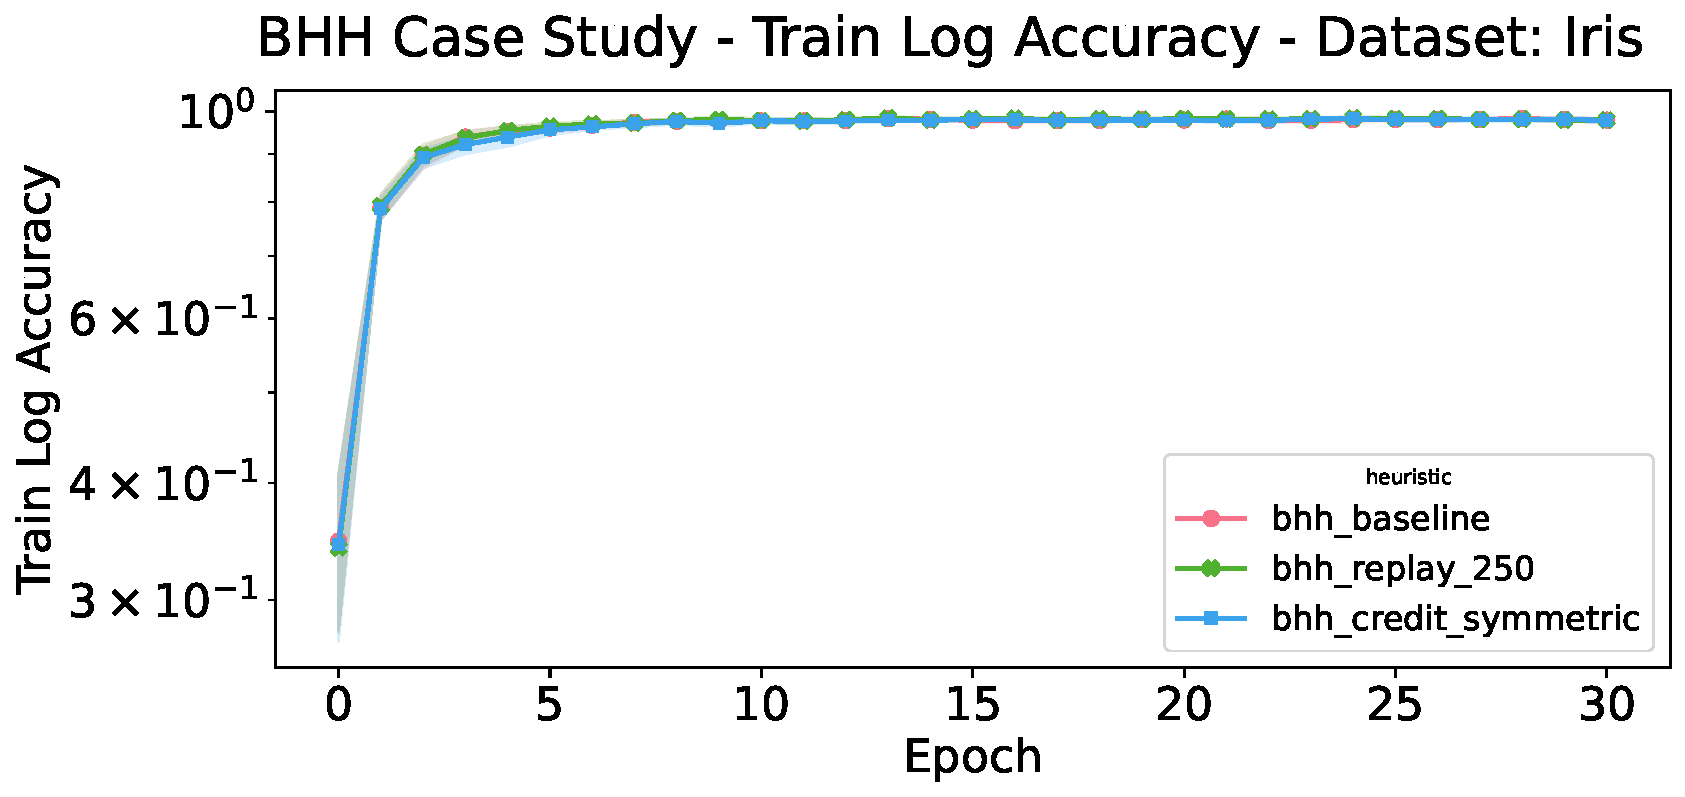
\includegraphics[width=1.0\textwidth]{case_study/metrics/figures/train/train_accuracy.pdf}
	\caption{The average training accuracy over 30 epochs, obtained from 30 runs of the case study on the behaviour of the \acs{BHH} on the iris dataset, illustrated in log scale.}
	\label{fig:results:case_study:train_accuracy}
\end{figure}

\begin{figure}[htpb]
	\centering
	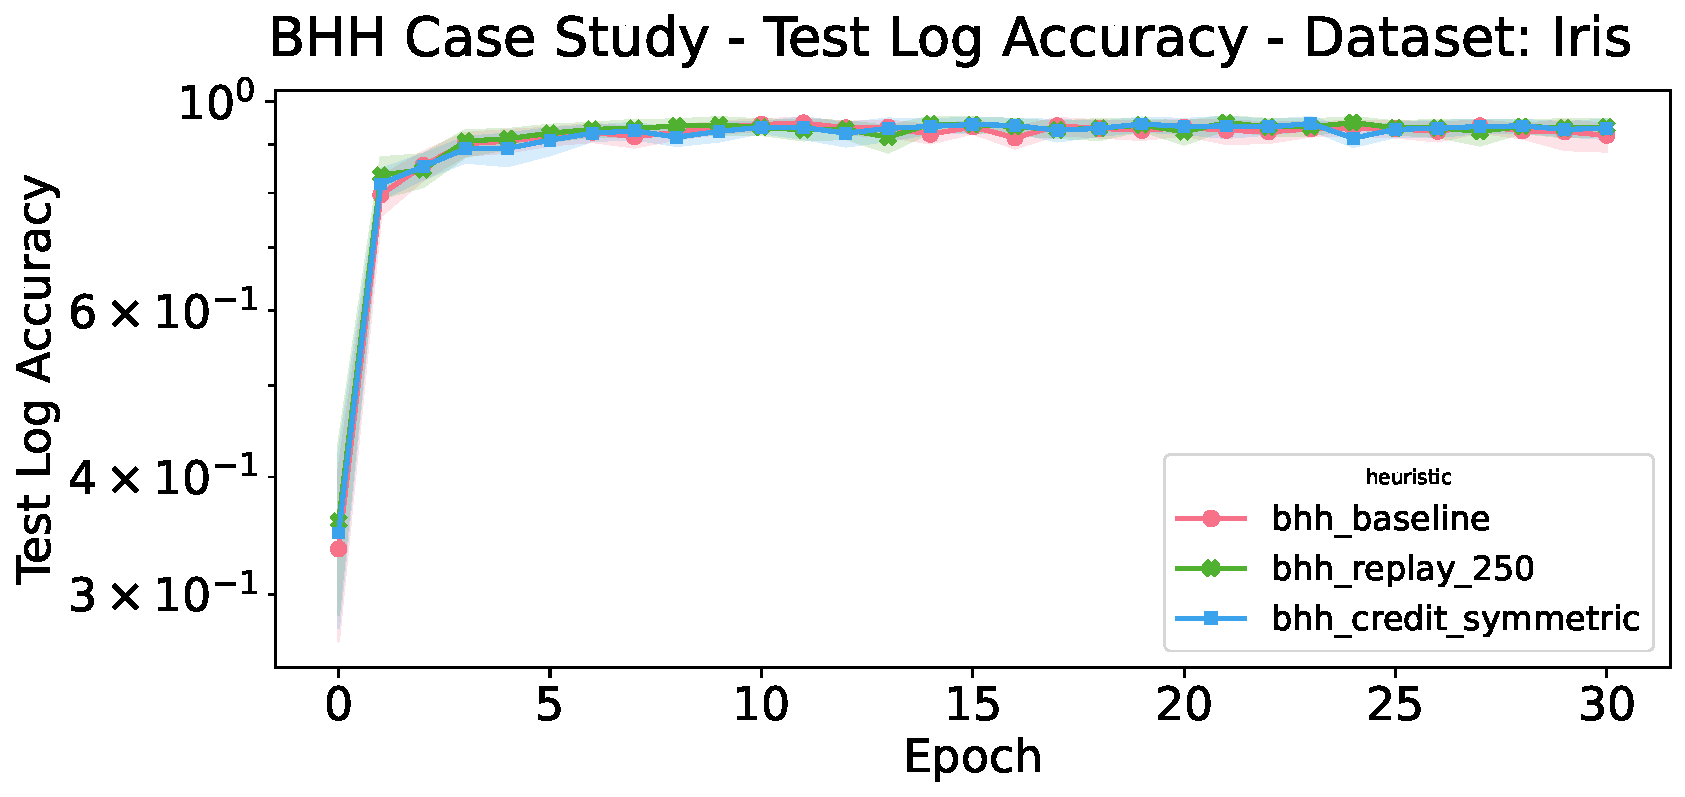
\includegraphics[width=1.0\textwidth]{case_study/metrics/figures/test/test_accuracy.pdf}
	\caption{The average test accuracy over 30 epochs, obtained from 30 runs of the case study on the behaviour of the \acs{BHH} on the iris dataset, illustrated in log scale.}
	\label{fig:results:case_study:test_accuracy}
\end{figure}


% %%%%%%%%%%%%%%%%%%%%%%%%%%%%%%%%%%%%%%%%%%%%%%%%%%%%%
% % PARAMS ALPHAS
% %%%%%%%%%%%%%%%%%%%%%%%%%%%%%%%%%%%%%%%%%%%%%%%%%%%%%

\subsection{Concentration Parameters}\label{sec:results:case_study:concentration_parameters}

To illustrate the learning process undergone by the \acs{BHH}, further investigation is required. Consider the concentration parameter $\boldsymbol{\alpha}$ that parameterises the \index{Dirichelet probability distribution}Dirichelet probability distribution, denoted $P(\boldsymbol{\theta} \vert \boldsymbol{\alpha})$, from which prior \textit{probabilities of selection probabilities} are sampled. Figures~\ref{fig:results:case_study:alpha:0}-\ref{fig:results:case_study:alpha:8} provide illustrations that show that change in values of the concentration parameter $\boldsymbol{\alpha}$, at indices 0, 6, 7, 8 respectively. Index 0, 6, 7, 8 represent the concentration parameters for the \acs{SGD}, \acs{Adam}, \acs{PSO} and \acs{GA} low-level heuristics respectively and only represent a subset of the concentration parameters in $\boldsymbol{\alpha}$ and the \index{heuristic pool}heuristic pool. Simular illustrations for the other indices in $\boldsymbol{\alpha}$ are left out for brevity as they contain similar illustrations.

\begin{figure}[htpb]
	\centering
	\includegraphics[width=1.0\textwidth]{case_study/params/figures/alphas/alpha[0].pdf}
	\caption{The average value of the concentration parameter $\alpha_{0}$ (\acs{SGD}) over 240 steps, obtained from 30 runs of the case study on the behaviour of the \acs{BHH} on the iris dataset, illustrated in log scale.}
	\label{fig:results:case_study:alpha:0}
\end{figure}

\begin{figure}[htpb]
	\centering
	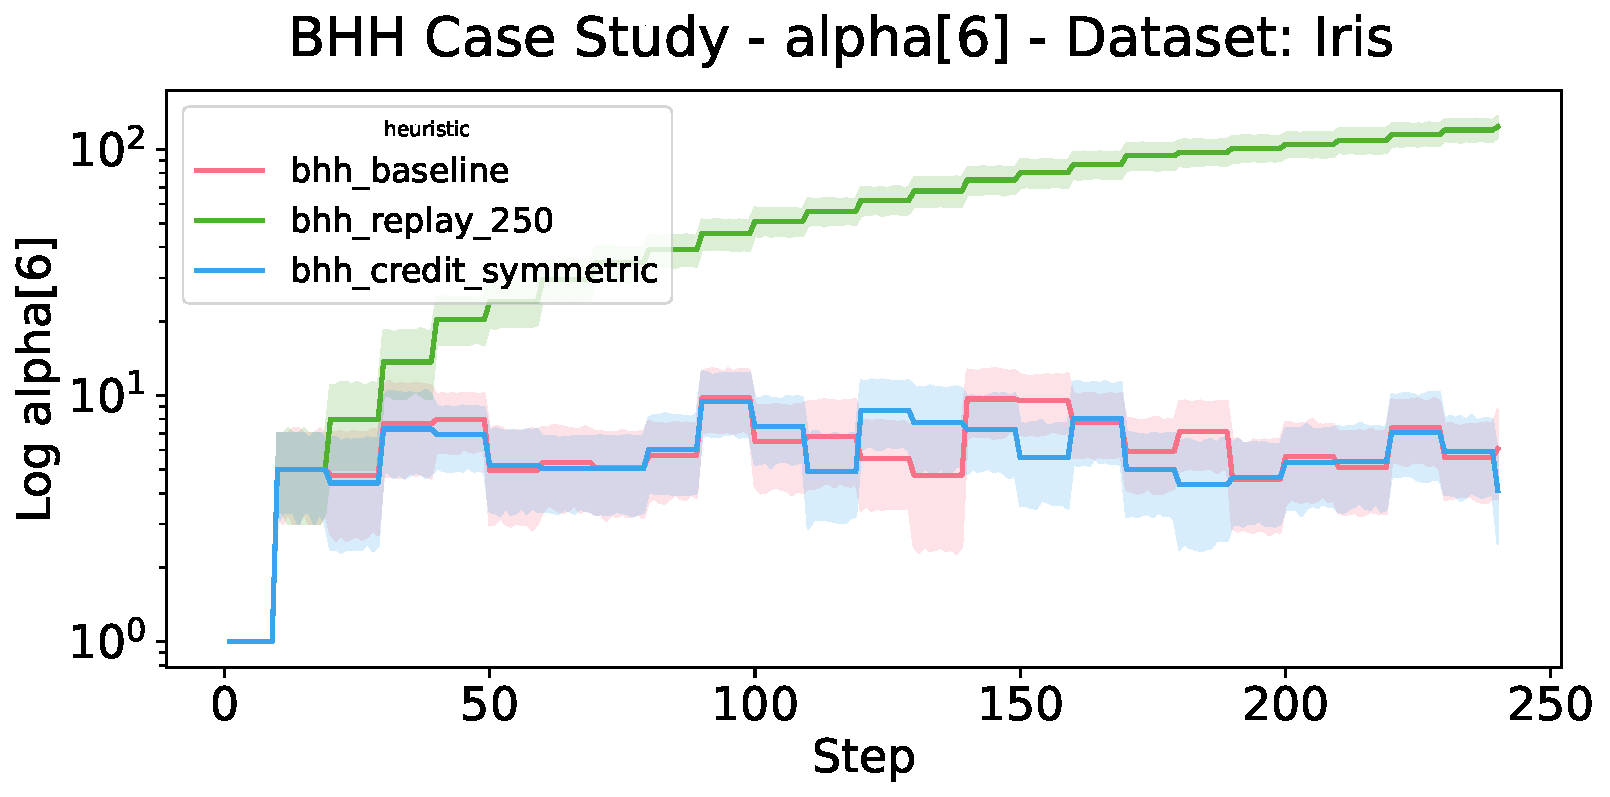
\includegraphics[width=1.0\textwidth]{case_study/params/figures/alphas/alpha[6].pdf}
	\caption{The average value of the concentration parameter $\alpha_{6}$ (\acs{Adam}) over 240 steps, obtained from 30 runs of the case study on the behaviour of the \acs{BHH} on the iris dataset, illustrated in log scale.}
	\label{fig:results:case_study:alpha:6}
\end{figure}

\begin{figure}[htpb]
	\centering
	\includegraphics[width=1.0\textwidth]{case_study/params/figures/alphas/alpha[7].pdf}
	\caption{The average value of the concentration parameter $\alpha_{7}$ (\acs{PSO}) over 240 steps, obtained from 30 runs of the case study on the behaviour of the \acs{BHH} on the iris dataset, illustrated in log scale.}
	\label{fig:results:case_study:alpha:7}
\end{figure}

\begin{figure}[htpb]
	\centering
	\includegraphics[width=1.0\textwidth]{case_study/params/figures/alphas/alpha[8].pdf}
	\caption{The average value of the concentration parameter $\alpha_{8}$ (\acs{GA}) over 240 steps, obtained from 30 runs of the case study on the behaviour of the \acs{BHH} on the iris dataset, illustrated in log scale.}
	\label{fig:results:case_study:alpha:8}
\end{figure}

The first logical observation to be made from Figures~\ref{fig:results:case_study:alpha:0}-\ref{fig:results:case_study:alpha:8} is the step-wise increasing nature of $\boldsymbol{\alpha}$ for the long memory configuration (denoted \textit{bhh\_replay\_250}), illustrated in green. Since the replay window size is sufficienty large to contain the performance log for all the steps executed in the training process, the \acs{BHH} does not forget past performances of low-level heuristics. The values in $\boldsymbol{\alpha}$ is never reset to its initial value of 1, and thus $\boldsymbol{\alpha}$ continues to increase throughout the training process. However, it should be noted that the rate and degree of change is different for different indices of $\boldsymbol{\alpha}$. The aforementioned observation is the first indicator of the learning process yielded by the \acs{BHH}. Heuristics that perform will will see their corresponding element in $\boldsymbol{\alpha}$ increase more rapidly that other heuristics that do not perform well.

The next observation that can be made is for the baseline configuration (denoted \textit{bhh\_baseline}) in red, and the symmetric credit assignment strategy configuration (denoted \textit{bhh\_credit\_symmetric}) in blue. Both these configurations see $\boldsymbol{\alpha}$ being reset to its initial value of 1 as regular intervals. This interval is represented by the \textit{reanalysis} window size. The reanalysis interval dictates the frequency at which Bayesian analysis is conducated on the performance log, mainted by the \acs{BHH}. Bayesian analysis is used to update $\boldsymbol{\alpha}$. As a result, small plateaus appear where $\boldsymbol{\alpha}$ does not change. Notice that $\boldsymbol{\alpha} \geq 1$ for multiple indices, even after reanalysis. This is because the same heuristic can be allocated to multiple entities, each contributing a minimum pseudo-count gain of 1 at the corresponding index in $\boldsymbol{\alpha}$ through the Bayesian analysis process. In a case where all 5 entities in the entity pool are allocated the same heuristic, for all 10 steps in the reanalysis windown, $\boldsymbol{\alpha} = 50$.

Furthermore, it is important to mention that a change in $\boldsymbol{\alpha}$ between reanalysis windows does not yet necessarily indicate that the \acs{BHH} is learning. The concentration parameter $\boldsymbol{\alpha}$ tracks the \textit{occurance} of the random event of observing heuristics (denoted $\boldsymbol{{H}}$). \index{heuristic}Heuristics can be observed as a result of good performance, by which the \acs{BHH} then learns to frequenctly reselect these \index{heuristic}heuristics again, or just by chance through the probabilistic sampling nature of the \acs{BHH}. Further investigation is required to illustrate the learning mechanism of the \acs{BHH}.



% %%%%%%%%%%%%%%%%%%%%%%%%%%%%%%%%%%%%%%%%%%%%%%%%%%%%%
% % PARAMS THETAS
% %%%%%%%%%%%%%%%%%%%%%%%%%%%%%%%%%%%%%%%%%%%%%%%%%%%%%

\subsection{Probabilities of Selection Probabilities}\label{sec:results:case_study:probs_of_select_probs}

This section provides a detailed investigation into the \textit{probabilities of selection probabilities}, denoted by $\boldsymbol{\theta}$, as it changes throughout the training process. As a reminder, the \acs{BHH} implements a Bayesian view of probabilistic modeling and thus, \index{heuristic}heuristic selection probabilities are defined by an underlying probablistic distribution themselves. The probability distribution of \index{heuristic}heuristic selection probabilities is denoted $P(\boldsymbol{\theta} \vert \boldsymbol{\alpha})$ and the prior \index{heuristic}heuristic selection probability distribution is denoted $P(\boldsymbol{H} \vert \boldsymbol{\theta})$.

Figures~\ref{fig:results:case_study:theta:0}-\ref{fig:results:case_study:theta:8} provide illustrations of the probabilities of the selection probabilities, sampled from the probability distribution $P(\boldsymbol{\theta} \vert \boldsymbol{\alpha})$ throughout the training process, and averaged over all 30 runs. These illustrations are presented in log scale. Similar to what is previously mentioned, \textit{probabilities of selection probabilities} at index 0, 6, 7, 8 represent the probabilities of selection probabilities for the \acs{SGD}, \acs{Adam}, \acs{PSO} and \acs{GA} low-level heuristics respectively and only represent a subset of the probabilities of selection probabilities in $\boldsymbol{\theta}$ and the \index{heuristic pool}heuristic pool. Once again, simular illustrations for the other indices in $\boldsymbol{\theta}$ are left out for brevity as they contain similar illustrations.

From the illustrations presented in Figures~\ref{fig:results:case_study:theta:0}-\ref{fig:results:case_study:theta:8}, a clearer picture off the learning process of the \acs{BHH} is formed. The first important observation to make is for the bhh\_replay\_250 configuration, presented in green. As a reminder, 10 low-level \index{heuristic}heuristics are included in the heuristic pool, yielding a probability of selection probability of 0.1 for each \index{heuristic}heuristic by the frequentist view of probabilistic modeling. Towards the end of the training process, the probability of selection probability converges back to the symmetrical, uniform probability distribution, yielding a probability of selection probability of 0.1 per \index{heuristic}heuristic. This can be explained as follows: most of the training progress is made in the early stages of the training process, and training stagnates towards the end of the training process. Since training stagnates, all heuristics, no matter their past performances, struggle to yield better solutions towards the end of the training process. As a result of stagnation, heuristics then struggle to yield credit allocations by means of the credit assignment strategy. In the case study experimental group, both the bhh\_baseline and bhh\_replay\_250 configurations make use of the \textit{ibest} credit assignment strategy. The \textit{ibest} credit assignment strategy allocates credit to the heuristic that provided the best performance for the current iteration/step and thus, towards the end of the training process, any random heuristic can yield the best iteration performance. However, since the bhh\_baseline has a short reanalysis interval, the concentration parameter $\boldsymbol{\alpha}$ gets reset to its default value of 1 more often than the bhh\_replay\_250 configuration, resulting in a probability distribution that is less narrow and thus explaining the larger variance of $\boldsymbol{\theta}$ throughout.

Another observation to make occurs in the first 30 steps of the training process. Notice how all three configurations mostly yield the same probabilities of selection probabilities in these first 30 steps. This can be explained as follows: all three configurations use a different random seed per run, but use the same random seed across configurations for the same runs. This is done so that any difference in the behaviour of the different \acs{BHH} configurations are then not a result of random sampling, but solely because of differences in their approaches. This is especially applicable to the initialisation process, where entities are randomly placed in the search space, as well as the early stages of training, where most of the training progress is made. It should be noted that, despite using the same random seed across configurations for the same runs, after about 30 steps, the behavioural changes between the configurations start the show. As a reminder, the bhh\_credit\_symmetric configuration, does not bias towards best performing \index{heuristic}heuristics and thus, where the bhh\_baseline and bhh\_replay\_250 configurations diverge from the behaviour of the bhh\_credit\_symmetric configuration, the difference in behaviour is proof of the effect of performance bias.

Finally, despite divergence in behaviour, the bhh\_baseline configuration and the bhh\_credit\_symmetric configuration both yield similar sporadic behaviour, much more so than with the bhh\_replay\_250 configuration. This can be attributed to a very small reanalysis window that contains very few samples to learn from (N=10). A small reanalysis window allows for more exploration, but can also yield greater variance of the probabilities of selection probabilities. Once again, any differences then in the behaviour of the  bhh\_baseline compared to the bhh\_credit\_symmetric configurations is proof of small performance exploitations.

\begin{figure}[htpb]
	\centering
	\includegraphics[width=1.0\textwidth]{case_study/params/figures/thetas/theta[0].pdf}
	\caption{The average sampled probability of the selection probability, denoted $\theta_{0}$ (\acs{SGD}), given concentration parameter $\alpha_{0}$. The probability of the selection probability is sampled from the probability distribution, denoted $P(\theta_{0} \vert \alpha_{0})$, over 240 steps, obtained from 30 runs of the case study on the behaviour of the \acs{BHH} on the iris dataset, illustrated in log scale.}
	\label{fig:results:case_study:theta:0}
\end{figure}

\begin{figure}[htpb]
	\centering
	\includegraphics[width=1.0\textwidth]{case_study/params/figures/thetas/theta[6].pdf}
	\caption{The average sampled probability of the selection probability, denoted $\theta_{6}$ (\acs{Adam}), given concentration parameter $\alpha_{6}$. The probability of the selection probability is sampled from the probability distribution, denoted $P(\theta_{6} \vert \alpha_{6})$, over 240 steps, obtained from 30 runs of the case study on the behaviour of the \acs{BHH} on the iris dataset, illustrated in log scale.}
	\label{fig:results:case_study:theta:6}
\end{figure}

\begin{figure}[htpb]
	\centering
	\includegraphics[width=1.0\textwidth]{case_study/params/figures/thetas/theta[7].pdf}
	\caption{The average sampled probability of the selection probability, denoted $\theta_{7}$ (\acs{PSO}), given concentration parameter $\alpha_{7}$. The probability of the selection probability is sampled from the probability distribution, denoted $P(\theta_{7} \vert \alpha_{7})$, over 240 steps, obtained from 30 runs of the case study on the behaviour of the \acs{BHH} on the iris dataset, illustrated in log scale.}
	\label{fig:results:case_study:theta:7}
\end{figure}

\begin{figure}[htpb]
	\centering
	\includegraphics[width=1.0\textwidth]{case_study/params/figures/thetas/theta[8].pdf}
	\caption{The average sampled probability of the selection probability, denoted $\theta_{8}$ (\acs{GA}), given concentration parameter $\alpha_{8}$. The probability of the selection probability is sampled from the probability distribution, denoted $P(\theta_{8} \vert \alpha_{8})$, over 240 steps, obtained from 30 runs of the case study on the behaviour of the \acs{BHH} on the iris dataset, illustrated in log scale.}
	\label{fig:results:case_study:theta:8}
\end{figure}

% %%%%%%%%%%%%%%%%%%%%%%%%%%%%%%%%%%%%%%%%%%%%%%%%%%%%%
% % PARAMS P_H (Priors)
% %%%%%%%%%%%%%%%%%%%%%%%%%%%%%%%%%%%%%%%%%%%%%%%%%%%%%

\subsection{Prior Selection Probabilities}\label{sec:results:case_study:prior_selec_prob}

This section provides a brief investigation into the \textit{prior \index{heuristic}heuristic selection probabilities}, that results from the probabilistic model implemented by the \acs{BHH}. The prior \index{heuristic}heuristic selection probability distribution is denoted $P(\boldsymbol{H} \vert \boldsymbol{\theta})$.

Figures~\ref{fig:results:case_study:p_H:0}-\ref{fig:results:case_study:p_H:8} provide illustrations of the prior\index{heuristic}heuristic selection probabilities, sampled from the \index{heuristic}heuristic selection probability distribution $P(\boldsymbol{H} \vert \boldsymbol{\theta})$ throughout the training process, and averaged over all 30 runs. Similar to before, these illustrations are also presented in log scale. The main observation to make from these figures is that they are much less sporadic than the figures presented for the probabilities of selection probabilities. This is because of the \textit{reselection} interval hyper-parameter. A reselection interval hyper-parameter is introduces to control the frequency by which new heuristics are allocated to each entity. Since the default \textit{reselection} interval is set to 10, the \index{heuristic}heuristic selection probabilities are only resampled at intervals of 10. These illustrations then simply yield rough approximations of the illustrations provided in Figures~\ref{fig:results:case_study:theta:0}-\ref{fig:results:case_study:theta:8} for the probabilities of selection probabilities. As such, the same observations and conclusions that are made in Section \ref{sec:results:case_study:probs_of_select_probs} also apply in this section.

Finally, it should be mentioned that at each step, the goal of the \acs{BHH} is to update these prior ``beliefs'' based on newly observed evidence of \index{heuristic}heuristic performances. Since these prior \index{heuristic}heuristic selection probabilities change over time, it can be concludes that the change in prior \index{heuristic}heuristic selection probabilities is a result of the learning mechanism of the \acs{BHH}. Furthermore, these prior \index{heuristic}heuristic selection probability distributions provide an opportunity to utilise prior knowledge by some expert to inject heuristic selection biases, even before training starts.

\begin{figure}[htpb]
	\centering
	\includegraphics[width=1.0\textwidth]{case_study/params/figures/p_H/p_H[0].pdf}
	\caption{The average sampled prior \index{heuristic}heuristic selection probability for \index{heuristic}heuristic $h_{0}$ (\acs{SGD}), given the probability of the selection probability, denoted by $\theta_{0}$. The prior \index{heuristic}heuristic selection probability is sampled from the prior \index{heuristic}heuristic selection probability distribution, denoted $P(h_{0} \vert \theta_{0})$, over 240 steps, obtained from 30 runs of the case study on the behaviour of the \acs{BHH} on the iris dataset, illustrated in log scale.}
	\label{fig:results:case_study:p_H:0}
\end{figure}

\begin{figure}[htpb]
	\centering
	\includegraphics[width=1.0\textwidth]{case_study/params/figures/p_H/p_H[6].pdf}
	\caption{The average sampled prior \index{heuristic}heuristic selection probability for \index{heuristic}heuristic $h_{6}$ (\acs{Adam}), given the probability of the selection probability, denoted by $\theta_{6}$. The prior \index{heuristic}heuristic selection probability is sampled from the prior \index{heuristic}heuristic selection probability distribution, denoted $P(h_{6} \vert \theta_{6})$, over 240 steps, obtained from 30 runs of the case study on the behaviour of the \acs{BHH} on the iris dataset, illustrated in log scale.}
	\label{fig:results:case_study:p_H:6}
\end{figure}

\begin{figure}[htpb]
	\centering
	\includegraphics[width=1.0\textwidth]{case_study/params/figures/p_H/p_H[7].pdf}
	\caption{The average sampled prior \index{heuristic}heuristic selection probability for \index{heuristic}heuristic $h_{7}$ (\acs{PSO}), given the probability of the selection probability, denoted by $\theta_{7}$. The prior \index{heuristic}heuristic selection probability is sampled from the prior \index{heuristic}heuristic selection probability distribution, denoted $P(h_{7} \vert \theta_{7})$, over 240 steps, obtained from 30 runs of the case study on the behaviour of the \acs{BHH} on the iris dataset, illustrated in log scale.}
	\label{fig:results:case_study:p_H:7}
\end{figure}

\begin{figure}[htpb]
	\centering
	\includegraphics[width=1.0\textwidth]{case_study/params/figures/p_H/p_H[8].pdf}
	\caption{The average sampled prior \index{heuristic}heuristic selection probability for \index{heuristic}heuristic $h_{8}$ (\acs{GA}), given the probability of the selection probability, denoted by $\theta_{8}$. The prior \index{heuristic}heuristic selection probability is sampled from the prior \index{heuristic}heuristic selection probability distribution, denoted $P(h_{8} \vert \theta_{8})$, over 240 steps, obtained from 30 runs of the case study on the behaviour of the \acs{BHH} on the iris dataset, illustrated in log scale.}
	\label{fig:results:case_study:p_H:8}
\end{figure}

% %%%%%%%%%%%%%%%%%%%%%%%%%%%%%%%%%%%%%%%%%%%%%%%%%%%%%
% % PARAMS P_HgEC (Posterior)
% %%%%%%%%%%%%%%%%%%%%%%%%%%%%%%%%%%%%%%%%%%%%%%%%%%%%%

\subsection{Posterior Selection Probabilities}\label{sec:results:case_study:posterior_selec_prob}

This section provides a brief investigation into the outcomes of the \textit{posterior heuristic selection probabilities} that forms the probabilistic model implemented by the \acs{BHH} from which new \index{heuristic}heuristics selections are sampled. The posterior \index{heuristic}heuristic selection probability distribution is denoted $P(\boldsymbol{H} \vert \boldsymbol{E}, \boldsymbol{C}; \boldsymbol{\theta}, \boldsymbol{\phi}, \boldsymbol{\psi})$, where $\boldsymbol{E}$ represents the vector representing the entities in the entity pool, and $\boldsymbol{C}$ represents the vector of performance criteria outcomes as implemented by the credit assignment strategy. Furthermore $\boldsymbol{\theta}, \boldsymbol{\phi}$ represent the probabilities of selection probabilities for the heuristics and entities respectively, and $\boldsymbol{\psi}$ represents the probability of observing a succesful credit allocation from the credit assignment strategy.

Figures~\ref{fig:results:case_study:p_HgEC:0:0}-\ref{fig:results:case_study:p_HgEC:0:8} provide illustrations of the calculated posterior \index{heuristic}heuristic selection probabilities, throughout the training process, and averaged over all 30 runs. Similar to before, these illustrations are also presented in log scale. The main observation to make from these figures is that these values do not actually yield probabilities. The reasons for this is because the probablistic model, defined by $P(\boldsymbol{H} \vert \boldsymbol{E}, \boldsymbol{C}; \boldsymbol{\theta}, \boldsymbol{\phi}, \boldsymbol{\psi})$, is evaluated for proportionality i.e. they are not normalised, and the log-sum-exp trick is used in order to maintain numerical stability. Instead, these values are used to parameterise a \index{Categorical probability distribution}Categorical probability distribution from which new \index{heuristic}heuristic selections are sampled.

The first noteworthy observation to make is for the bhh\_replay\_250 configuration. From Figures~\ref{fig:results:case_study:p_HgEC:0:0}-\ref{fig:results:case_study:p_HgEC:0:8}, it can be seen that the posterior heuristic selection probabilities stagnate. As previously mentioned, this is a result of training stagnation later in the training process. As a result, fewer and fewer improvements to the current best solutions are found, thus yielding a case where heuristic selection bias is based mostly on past performances obtained from a large reanalysis window.

Furthermore, the posterior heuristic selection probability distribution is conditional on the occurance of a specific entity that the potential \index{heuristic}heuristic will be applied to, as well as a specific performance criteria enforced by a specific credit assignment strategy. This means that \index{heuristic}heuristic selection is specific to each entity. A particular \index{heuristic}heuristic might be good for one entity, but not for another. This is a strong characteristic of the \acs{BHH}, as it learns to apply the correct \index{heuristic}heuristic to the correct entity at the correct point in the training process.

Finally, the posterior heuristic selection probabilities oscillate much less and are much less sporadic than their prior heuristic selection probability equivalents. This is a result of the information that is added by the conditionality on entity and performance criteria.

\begin{figure}[htpb]
	\centering
	\includegraphics[width=1.0\textwidth]{case_study/params/figures/p_HgEC/p_HgEC[0][0].pdf}
	\caption{The average proportional posterior selection probability for \index{heuristic}heuristic $h_{0}$ (\acs{SGD}), given the application to entity $e_{0}$ and requiring a successful credit allocation ($\gamma_{1}$) from the \textit{ibest} credit assignment strategy. The proportional posterior selection probability is calculated from the probabilistic model, denoted $P(h_{0} \vert e_{0}, \gamma_{1})$, over 240 steps, and obtained from 30 runs of the case study on the behaviour of the \acs{BHH} on the iris dataset, illustrated in log scale.}
	\label{fig:results:case_study:p_HgEC:0:0}
\end{figure}

\begin{figure}[htpb]
	\centering
	\includegraphics[width=1.0\textwidth]{case_study/params/figures/p_HgEC/p_HgEC[0][6].pdf}
	\caption{The average proportional posterior selection probability for \index{heuristic}heuristic $h_{6}$ (\acs{Adam}), given the application to entity $e_{0}$ and requiring a successful credit allocation ($\gamma_{1}$) from the \textit{ibest} credit assignment strategy. The proportional posterior selection probability is calculated from the probabilistic model, denoted $P(h_{6} \vert e_{0}, \gamma_{1})$, over 240 steps, and obtained from 30 runs of the case study on the behaviour of the \acs{BHH} on the iris dataset, illustrated in log scale.}
	\label{fig:results:case_study:p_HgEC:0:6}
\end{figure}

\begin{figure}[htpb]
	\centering
	\includegraphics[width=1.0\textwidth]{case_study/params/figures/p_HgEC/p_HgEC[0][7].pdf}
	\caption{The average proportional posterior selection probability for \index{heuristic}heuristic $h_{7}$ (\acs{PSO}), given the application to entity $e_{0}$ and requiring a successful credit allocation ($\gamma_{1}$) from the \textit{ibest} credit assignment strategy. The proportional posterior selection probability is calculated from the probabilistic model, denoted $P(h_{7} \vert e_{0}, \gamma_{1})$, over 240 steps, and obtained from 30 runs of the case study on the behaviour of the \acs{BHH} on the iris dataset, illustrated in log scale.}
	\label{fig:results:case_study:p_HgEC:0:7}
\end{figure}

\begin{figure}[htpb]
	\centering
	\includegraphics[width=1.0\textwidth]{case_study/params/figures/p_HgEC/p_HgEC[0][8].pdf}
	\caption{The average proportional posterior selection probability for \index{heuristic}heuristic $h_{8}$ (\acs{GA}), given the application to entity $e_{0}$ and requiring a successful credit allocation ($\gamma_{1}$) from the \textit{ibest} credit assignment strategy. The proportional posterior selection probability is calculated from the probabilistic model, denoted $P(h_{8} \vert e_{0}, \gamma_{1})$, over 240 steps, and obtained from 30 runs of the case study on the behaviour of the \acs{BHH} on the iris dataset, illustrated in log scale.}
	\label{fig:results:case_study:p_HgEC:0:8}
\end{figure}

From the observations made in Sections~\ref{sec:results:case_study:performance_metrics}-\ref{sec:results:case_study:posterior_selec_prob}, it can be concluded that the \acs{BHH} is able to succesfully train the underlying \acs{FFNN}. Furthermore it can be concluded that the learning mechanism implemented by the \acs{BHH} is able to exploit minor performance biases and thus, the \acs{BHH} is able to correctly allocate the correct heuristic to the correct entity at the correct time in the training process.

%%%%%%%%%%%%%%%%%%%%%%%%%%%%%%%%%%%%%%%%%%%%%%%%%%%%%%%%%%%%%%%5
% BHH vs. Low-Level Heuristics
%%%%%%%%%%%%%%%%%%%%%%%%%%%%%%%%%%%%%%%%%%%%%%%%%%%%%%%%%%%%%%%5
\section{BHH vs. Low-Level Heuristics}\label{sec:results:standalone}

This section provides the empirical results for the experimental group that compares the performance of the \acs{BHH} to the performance of the individual, standalone, low-level heuristics. Detailed discussions and illustrations follow. As a reminder, the set of low-level heuristics include a number of gradient-based heuristics and a number of meta-heuristics. Three different variants of the \acs{BHH} is included in the experiment, including the \acs{BHH} baseline configuration with a \index{heuristic pool}heuristic pool that contains all the low-level heuristics (denoted bhh\_all), the \acs{BHH} configuration with a \index{heuristic pool}heuristic pool that contains only gradient-based \index{heuristic}heuristics (denoted bhh\_gd), and finally, a \acs{BHH} configuration with a \index{heuristic pool}heuristics pool that contains only \index{meta-heuristic}meta-heuristics (denoted bhh\_mh).

Table~\ref{tab:results:standalone:metrics:test_loss} presents the empirical results for this experimental group, showing the average test loss and statistics for all the low-level heuristics, compared to the three variants of the \acs{BHH} that was implemented. The test loss that is reported in Table~\ref{tab:results:standalone:metrics:test_loss} reflects on the test loss achieved at the last epoch of training, across all datasets, averaged over all independent runs.

% Table generated by Excel2LaTeX from sheet 'results - test - loss'
\begin{table}[H]
	\centering
	\caption{Empirical results showing average test loss and statistics for different low-level \index{heuristic}heuristics compared to 3 \index{heuristic pool}heuristic pool variants of the baseline \acs{BHH} across multiple datasets, for all runs, at the last epoch.}
	\label{tab:results:standalone:metrics:test_loss}%
	\par\bigskip
	\resizebox{\textwidth}{!}{
		\begin{tabular}{rlccc|c|c|c|c|c|ccccc}
			epoch                                                                          & 30                 &                                                                                &                                                                                & \multicolumn{1}{r}{}                                                           & \multicolumn{1}{r}{}                            & \multicolumn{1}{r}{}                                                           & \multicolumn{1}{r}{}                            & \multicolumn{1}{r}{}                                                           & \multicolumn{1}{r}{}                            &                                                 &                                                 &                                                 &                                                 &                                                 \\
			                                                                               &                    &                                                                                &                                                                                & \multicolumn{1}{r}{}                                                           & \multicolumn{1}{r}{}                            & \multicolumn{1}{r}{}                                                           & \multicolumn{1}{r}{}                            & \multicolumn{1}{r}{}                                                           & \multicolumn{1}{r}{}                            &                                                 &                                                 &                                                 &                                                 &                                                 \\
			                                                                               &                    & \multicolumn{1}{l}{\textbf{heuristic}}                                         &                                                                                & \multicolumn{1}{r}{}                                                           & \multicolumn{1}{r}{}                            & \multicolumn{1}{r}{}                                                           & \multicolumn{1}{r}{}                            & \multicolumn{1}{r}{}                                                           & \multicolumn{1}{r}{}                            &                                                 &                                                 &                                                 &                                                 &                                                 \\
			\cmidrule{3-3}\cmidrule{6-6}\cmidrule{8-8}\cmidrule{10-10}    \textbf{dataset} & \textbf{statistic} & \textbf{adagrad}                                                               & \textbf{adam}                                                                  & \textbf{nag}                                                                   & \textbf{bhh\_gd}                                & \textbf{rmsprop}                                                               & \textbf{bhh\_all}                               & \textbf{adadelta}                                                              & \textbf{bhh\_mh}                                & \textbf{ga}                                     & \textbf{sgd}                                    & \textbf{pso}                                    & \textbf{momentum}                               & \textbf{de}                                     \\
			\midrule
			abalone                                                                        & count              & 30                                                                             & 30                                                                             & 30                                                                             & 30                                              & 30                                                                             & 30                                              & 30                                                                             & 30                                              & 30                                              & 30                                              & 30                                              & 30                                              & 30                                              \\
			                                                                               & avg                & \cellcolor[rgb]{ .506,  .776,  .486}1.967785                                   & \cellcolor[rgb]{ .494,  .773,  .486}1.965134827                                & \cellcolor[rgb]{ .765,  .851,  .502}2.0156043                                  & \cellcolor[rgb]{ .749,  .847,  .502}2.012517173 & \cellcolor[rgb]{ .388,  .745,  .482}\textcolor[rgb]{ 0,  .38,  0}{1.94553315}  & \cellcolor[rgb]{ 1,  .922,  .518}2.058704583    & \cellcolor[rgb]{ .788,  .859,  .502}2.019921077                                & \cellcolor[rgb]{ .996,  .827,  .502}2.29420573  & \cellcolor[rgb]{ .984,  .612,  .459}2.81545685  & \cellcolor[rgb]{ .992,  .773,  .49}2.42804241   & \cellcolor[rgb]{ .98,  .522,  .443}3.038417873  & \cellcolor[rgb]{ .992,  .745,  .486}2.494169393 & \cellcolor[rgb]{ .973,  .412,  .42}3.295858177  \\
			                                                                               & std                & 0.031577789                                                                    & 0.034949967                                                                    & 0.034657443                                                                    & 0.068121366                                     & 0.035183664                                                                    & 0.087594488                                     & 0.034405331                                                                    & 0.055085207                                     & 0.055148148                                     & 0.028810924                                     & 0.293755503                                     & 0.029086341                                     & 0.016489872                                     \\
			adult                                                                          & count              & 30                                                                             & 30                                                                             & 30                                                                             & 30                                              & 30                                                                             & 30                                              & 30                                                                             & 30                                              & 30                                              & 30                                              & 30                                              & 30                                              & 30                                              \\
			                                                                               & avg                & \cellcolor[rgb]{ 1,  .922,  .518}0.346737798                                   & \cellcolor[rgb]{ 1,  .922,  .518}0.38233353                                    & \cellcolor[rgb]{ .388,  .745,  .482}\textcolor[rgb]{ 0,  .38,  0}{0.313320884} & \cellcolor[rgb]{ .788,  .859,  .502}0.335180995 & \cellcolor[rgb]{ .933,  .902,  .514}0.343292783                                & \cellcolor[rgb]{ .973,  .412,  .42}586.2065996  & \cellcolor[rgb]{ .467,  .765,  .486}0.317677033                                & \cellcolor[rgb]{ 1,  .922,  .518}0.363543899    & \cellcolor[rgb]{ 1,  .922,  .518}0.392047161    & \cellcolor[rgb]{ .388,  .745,  .482}0.313329677 & \cellcolor[rgb]{ 1,  .922,  .518}1.217724345    & \cellcolor[rgb]{ .388,  .745,  .482}0.313444396 & \cellcolor[rgb]{ 1,  .922,  .518}0.639695856    \\
			                                                                               & std                & 0.003704238                                                                    & 0.018067239                                                                    & 0.000510377                                                                    & 0.043628962                                     & 0.014659665                                                                    & 1261.204704                                     & 0.005277776                                                                    & 0.020803371                                     & 0.020086997                                     & 0.000411017                                     & 0.496591684                                     & 0.0003947                                       & 0.042558869                                     \\
			air quality                                                                    & count              & 30                                                                             & 30                                                                             & 30                                                                             & 30                                              & 30                                                                             & 30                                              & 30                                                                             & 30                                              & 30                                              & 30                                              & 30                                              & 30                                              & 30                                              \\
			                                                                               & avg                & \cellcolor[rgb]{ .651,  .82,  .494}0.256871193                                 & \cellcolor[rgb]{ .827,  .871,  .506}0.260623969                                & \cellcolor[rgb]{ .647,  .82,  .494}0.256829053                                 & \cellcolor[rgb]{ 1,  .922,  .518}0.264177871    & \cellcolor[rgb]{ .388,  .745,  .482}\textcolor[rgb]{ 0,  .38,  0}{0.251334045} & \cellcolor[rgb]{ .996,  .827,  .502}0.272859303 & \cellcolor[rgb]{ .647,  .82,  .494}0.256781683                                 & \cellcolor[rgb]{ .976,  .914,  .514}0.263703859 & \cellcolor[rgb]{ .996,  .792,  .494}0.275862527 & \cellcolor[rgb]{ .988,  .69,  .475}0.285172782  & \cellcolor[rgb]{ .984,  .608,  .459}0.292264593 & \cellcolor[rgb]{ .984,  .604,  .459}0.292851261 & \cellcolor[rgb]{ .973,  .412,  .42}0.309698115  \\
			                                                                               & std                & 0.007475522                                                                    & 0.008912099                                                                    & 0.005955119                                                                    & 0.011452365                                     & 0.007814891                                                                    & 0.016310047                                     & 0.00630808                                                                     & 0.007306605                                     & 0.008162884                                     & 0.014769128                                     & 0.022648597                                     & 0.016417541                                     & 0.017044223                                     \\
			bank                                                                           & count              & 30                                                                             & 30                                                                             & 30                                                                             & 30                                              & 30                                                                             & 30                                              & 30                                                                             & 30                                              & 30                                              & 30                                              & 30                                              & 30                                              & 30                                              \\
			                                                                               & avg                & \cellcolor[rgb]{ .459,  .765,  .486}0.209641222                                & \cellcolor[rgb]{ .4,  .745,  .482}0.206461621                                  & \cellcolor[rgb]{ .588,  .8,  .49}0.2164275                                     & \cellcolor[rgb]{ .588,  .8,  .49}0.21643132     & \cellcolor[rgb]{ .388,  .745,  .482}\textcolor[rgb]{ 0,  .38,  0}{0.205779476} & \cellcolor[rgb]{ 1,  .886,  .514}0.245610465    & \cellcolor[rgb]{ .627,  .812,  .494}0.218599386                                & \cellcolor[rgb]{ .996,  .839,  .502}0.256171151 & \cellcolor[rgb]{ .988,  .686,  .475}0.28813827  & \cellcolor[rgb]{ 1,  .922,  .518}0.238179998    & \cellcolor[rgb]{ .973,  .412,  .42}0.345448185  & \cellcolor[rgb]{ 1,  .922,  .518}0.238550439    & \cellcolor[rgb]{ .976,  .424,  .424}0.343699166 \\
			                                                                               & std                & 0.004750498                                                                    & 0.004040969                                                                    & 0.005944898                                                                    & 0.004889433                                     & 0.005654034                                                                    & 0.064531685                                     & 0.003821749                                                                    & 0.010550504                                     & 0.012801143                                     & 0.005568018                                     & 0.033990143                                     & 0.004820977                                     & 0.028120079                                     \\
			bike                                                                           & count              & 30                                                                             & 30                                                                             & 30                                                                             & 30                                              & 30                                                                             & 30                                              & 30                                                                             & 30                                              & 30                                              & 30                                              & 30                                              & 30                                              & 30                                              \\
			                                                                               & avg                & \cellcolor[rgb]{ .388,  .745,  .482}\textcolor[rgb]{ 0,  .38,  0}{0.045805387} & \cellcolor[rgb]{ .592,  .804,  .494}0.068179412                                & \cellcolor[rgb]{ .882,  .886,  .51}0.099539486                                 & \cellcolor[rgb]{ .467,  .765,  .486}0.054496914 & \cellcolor[rgb]{ 1,  .922,  .518}0.112259627                                   & \cellcolor[rgb]{ .565,  .796,  .49}0.065136647  & \cellcolor[rgb]{ .588,  .8,  .49}0.06793708                                    & \cellcolor[rgb]{ 1,  .902,  .514}0.11787523     & \cellcolor[rgb]{ .992,  .761,  .486}0.153095534 & \cellcolor[rgb]{ .992,  .733,  .482}0.159868436 & \cellcolor[rgb]{ .992,  .773,  .49}0.150273084  & \cellcolor[rgb]{ .992,  .725,  .482}0.161397393 & \cellcolor[rgb]{ .973,  .412,  .42}0.239867227  \\
			                                                                               & std                & 0.001725608                                                                    & 0.068117237                                                                    & 0.001754469                                                                    & 0.005239285                                     & 0.103490928                                                                    & 0.019626763                                     & 0.002076596                                                                    & 0.005954748                                     & 0.005079692                                     & 0.002759                                        & 0.025177188                                     & 0.003354245                                     & 0.039791214                                     \\
			car                                                                            & count              & 30                                                                             & 30                                                                             & 30                                                                             & 30                                              & 30                                                                             & 30                                              & 30                                                                             & 30                                              & 30                                              & 30                                              & 30                                              & 30                                              & 30                                              \\
			                                                                               & avg                & \cellcolor[rgb]{ .729,  .843,  .502}0.202726327                                & \cellcolor[rgb]{ .388,  .745,  .482}\textcolor[rgb]{ 0,  .38,  0}{0.09724452}  & \cellcolor[rgb]{ .867,  .882,  .51}0.245363623                                 & \cellcolor[rgb]{ .62,  .812,  .494}0.16895294   & \cellcolor[rgb]{ .408,  .749,  .482}0.103937737                                & \cellcolor[rgb]{ .58,  .8,  .49}0.15718728      & \cellcolor[rgb]{ 1,  .922,  .518}0.285888989                                   & \cellcolor[rgb]{ .992,  .733,  .482}0.489062582 & \cellcolor[rgb]{ .98,  .502,  .439}0.737354357  & \cellcolor[rgb]{ .98,  .533,  .443}0.703539757  & \cellcolor[rgb]{ .988,  .667,  .471}0.563173207 & \cellcolor[rgb]{ .98,  .506,  .439}0.73217904   & \cellcolor[rgb]{ .973,  .412,  .42}0.833160108  \\
			                                                                               & std                & 0.018356416                                                                    & 0.023870777                                                                    & 0.028744869                                                                    & 0.025441117                                     & 0.031133074                                                                    & 0.033710554                                     & 0.027353972                                                                    & 0.076505599                                     & 0.062600847                                     & 0.052091474                                     & 0.157928484                                     & 0.042705727                                     & 0.074182791                                     \\
			diabetic                                                                       & count              & 30                                                                             & 30                                                                             & 30                                                                             & 30                                              & 30                                                                             & 30                                              & 30                                                                             & 30                                              & 30                                              & 30                                              & 30                                              & 30                                              & 30                                              \\
			                                                                               & avg                & \cellcolor[rgb]{ .694,  .831,  .498}0.889537739                                & \cellcolor[rgb]{ 1,  .898,  .514}0.919339482                                   & \cellcolor[rgb]{ .388,  .745,  .482}\textcolor[rgb]{ 0,  .38,  0}{0.880898965} & \cellcolor[rgb]{ .98,  .914,  .514}0.897587026  & \cellcolor[rgb]{ .918,  .894,  .51}0.895749019                                 & \cellcolor[rgb]{ .973,  .412,  .42}1.298319185  & \cellcolor[rgb]{ .49,  .773,  .486}0.883864405                                 & \cellcolor[rgb]{ 1,  .902,  .518}0.913694494    & \cellcolor[rgb]{ .996,  .843,  .506}0.961291775 & \cellcolor[rgb]{ .976,  .914,  .514}0.897429714 & \cellcolor[rgb]{ .996,  .835,  .502}0.966103049 & \cellcolor[rgb]{ 1,  .922,  .518}0.898038783    & \cellcolor[rgb]{ .988,  .694,  .475}1.077362637 \\
			                                                                               & std                & 0.004272255                                                                    & 0.00981794                                                                     & 0.003758597                                                                    & 0.010748722                                     & 0.004045488                                                                    & 0.659754133                                     & 0.004759234                                                                    & 0.008388702                                     & 0.00657199                                      & 0.003551413                                     & 0.016450474                                     & 0.002801135                                     & 0.0391395                                       \\
			fish toxicity                                                                  & count              & 30                                                                             & 30                                                                             & 30                                                                             & 30                                              & 30                                                                             & 30                                              & 30                                                                             & 30                                              & 30                                              & 30                                              & 30                                              & 30                                              & 30                                              \\
			                                                                               & avg                & \cellcolor[rgb]{ .588,  .8,  .49}0.09908239                                    & \cellcolor[rgb]{ .451,  .761,  .482}0.097196901                                & \cellcolor[rgb]{ .831,  .871,  .506}0.10233624                                 & \cellcolor[rgb]{ 1,  .91,  .518}0.105584544     & \cellcolor[rgb]{ .388,  .745,  .482}\textcolor[rgb]{ 0,  .38,  0}{0.096326802} & \cellcolor[rgb]{ 1,  .922,  .518}0.104598099    & \cellcolor[rgb]{ .773,  .855,  .502}0.101567158                                & \cellcolor[rgb]{ .976,  .914,  .514}0.104293618 & \cellcolor[rgb]{ 1,  .863,  .506}0.109342435    & \cellcolor[rgb]{ .976,  .475,  .435}0.139280655 & \cellcolor[rgb]{ 1,  .855,  .506}0.109946059    & \cellcolor[rgb]{ .973,  .412,  .42}0.144088336  & \cellcolor[rgb]{ .992,  .733,  .482}0.119344204 \\
			                                                                               & std                & 0.008463336                                                                    & 0.006948088                                                                    & 0.007611236                                                                    & 0.008228438                                     & 0.008021585                                                                    & 0.008136956                                     & 0.008882708                                                                    & 0.00895412                                      & 0.008990894                                     & 0.012326524                                     & 0.012481736                                     & 0.012407706                                     & 0.0130782                                       \\
			forest fires                                                                   & count              & 30                                                                             & 30                                                                             & 30                                                                             & 30                                              & 30                                                                             & 30                                              & 30                                                                             & 30                                              & 30                                              & 30                                              & 30                                              & 30                                              & 30                                              \\
			                                                                               & avg                & \cellcolor[rgb]{ 1,  .922,  .518}0.064321917                                   & \cellcolor[rgb]{ .557,  .792,  .49}0.052658676                                 & \cellcolor[rgb]{ .851,  .878,  .506}0.05923886                                 & \cellcolor[rgb]{ .824,  .871,  .506}0.058617148 & \cellcolor[rgb]{ 1,  .922,  .518}0.062552555                                   & \cellcolor[rgb]{ 1,  .89,  .514}0.080966845     & \cellcolor[rgb]{ .388,  .745,  .482}\textcolor[rgb]{ 0,  .38,  0}{0.048831474} & \cellcolor[rgb]{ .976,  .914,  .514}0.06209696  & \cellcolor[rgb]{ .553,  .792,  .49}0.05260701   & \cellcolor[rgb]{ .992,  .722,  .482}0.180571383 & \cellcolor[rgb]{ 1,  .914,  .518}0.069210426    & \cellcolor[rgb]{ .992,  .706,  .478}0.188476672 & \cellcolor[rgb]{ .973,  .412,  .42}0.359831599  \\
			                                                                               & std                & 0.039911806                                                                    & 0.039243672                                                                    & 0.031685801                                                                    & 0.034163415                                     & 0.039170629                                                                    & 0.069099845                                     & 0.032095867                                                                    & 0.038470671                                     & 0.025957821                                     & 0.008365929                                     & 0.047244856                                     & 0.010081381                                     & 0.089999905                                     \\
			housing                                                                        & count              & 30                                                                             & 30                                                                             & 30                                                                             & 30                                              & 30                                                                             & 30                                              & 30                                                                             & 30                                              & 30                                              & 30                                              & 30                                              & 30                                              & 30                                              \\
			                                                                               & avg                & \cellcolor[rgb]{ .518,  .78,  .486}0.088925893                                 & \cellcolor[rgb]{ .404,  .749,  .482}0.08481865                                 & \cellcolor[rgb]{ .612,  .808,  .494}0.092269667                                & \cellcolor[rgb]{ .69,  .831,  .498}0.095072459  & \cellcolor[rgb]{ .388,  .745,  .482}\textcolor[rgb]{ 0,  .38,  0}{0.08422333}  & \cellcolor[rgb]{ .663,  .824,  .498}0.094078934 & \cellcolor[rgb]{ 1,  .922,  .518}0.105999965                                   & \cellcolor[rgb]{ 1,  .867,  .51}0.116883814     & \cellcolor[rgb]{ .996,  .812,  .498}0.127851649 & \cellcolor[rgb]{ .984,  .576,  .455}0.173521216 & \cellcolor[rgb]{ .992,  .722,  .482}0.145240159 & \cellcolor[rgb]{ .984,  .588,  .455}0.171302372 & \cellcolor[rgb]{ .973,  .412,  .42}0.205724786  \\
			                                                                               & std                & 0.012490666                                                                    & 0.011213172                                                                    & 0.015551947                                                                    & 0.014823695                                     & 0.014924594                                                                    & 0.017302471                                     & 0.018700331                                                                    & 0.019460369                                     & 0.020192262                                     & 0.022837541                                     & 0.029813905                                     & 0.017916976                                     & 0.036445189                                     \\
			iris                                                                           & count              & 30                                                                             & 30                                                                             & 30                                                                             & 30                                              & 30                                                                             & 30                                              & 30                                                                             & 30                                              & 30                                              & 30                                              & 30                                              & 30                                              & 30                                              \\
			                                                                               & avg                & \cellcolor[rgb]{ .788,  .859,  .502}0.216138929                                & \cellcolor[rgb]{ .514,  .78,  .486}0.120305813                                 & \cellcolor[rgb]{ .416,  .753,  .482}0.084967127                                & \cellcolor[rgb]{ 1,  .855,  .506}0.372908547    & \cellcolor[rgb]{ .388,  .745,  .482}\textcolor[rgb]{ 0,  .38,  0}{0.075287772} & \cellcolor[rgb]{ .859,  .878,  .506}0.241094806 & \cellcolor[rgb]{ .996,  .808,  .498}0.426015649                                & \cellcolor[rgb]{ .686,  .831,  .498}0.180917533 & \cellcolor[rgb]{ 1,  .922,  .518}0.289495446    & \cellcolor[rgb]{ .992,  .773,  .49}0.469415404  & \cellcolor[rgb]{ .973,  .412,  .42}0.896458149  & \cellcolor[rgb]{ .992,  .745,  .486}0.502796506 & \cellcolor[rgb]{ .98,  .494,  .435}0.802733988  \\
			                                                                               & std                & 0.059156887                                                                    & 0.097731271                                                                    & 0.041820159                                                                    & 1.119111663                                     & 0.045657899                                                                    & 0.295227964                                     & 0.071608458                                                                    & 0.163729792                                     & 0.117435582                                     & 0.087556703                                     & 0.844445785                                     & 0.072001841                                     & 0.684394699                                     \\
			mushroom                                                                       & count              & 30                                                                             & 30                                                                             & 30                                                                             & 30                                              & 30                                                                             & 30                                              & 30                                                                             & 30                                              & 30                                              & 30                                              & 30                                              & 30                                              & 30                                              \\
			                                                                               & avg                & \cellcolor[rgb]{ .549,  .792,  .49}0.002577835                                 & \cellcolor[rgb]{ .467,  .765,  .486}0.001321295                                & \cellcolor[rgb]{ 1,  .922,  .518}0.009417256                                   & \cellcolor[rgb]{ .439,  .757,  .482}0.000906998 & \cellcolor[rgb]{ .388,  .745,  .482}\textcolor[rgb]{ 0,  .38,  0}{8.30695E-05} & \cellcolor[rgb]{ .718,  .839,  .498}0.005152476 & \cellcolor[rgb]{ .655,  .82,  .494}0.00417499                                  & \cellcolor[rgb]{ 1,  .871,  .51}0.077415858     & \cellcolor[rgb]{ .984,  .561,  .451}0.489160105 & \cellcolor[rgb]{ .996,  .796,  .494}0.179705445 & \cellcolor[rgb]{ 1,  .886,  .514}0.061137885    & \cellcolor[rgb]{ .992,  .749,  .486}0.241811308 & \cellcolor[rgb]{ .973,  .412,  .42}0.687017333  \\
			                                                                               & std                & 0.000662841                                                                    & 0.004905902                                                                    & 0.002279151                                                                    & 0.001259819                                     & 6.96496E-05                                                                    & 0.012039998                                     & 0.000905097                                                                    & 0.019865901                                     & 0.024593143                                     & 0.009208458                                     & 0.06033175                                      & 0.012790223                                     & 0.01638976                                      \\
			parkinsons                                                                     & count              & 30                                                                             & 30                                                                             & 30                                                                             & 30                                              & 30                                                                             & 30                                              & 30                                                                             & 30                                              & 30                                              & 30                                              & 30                                              & 30                                              & 30                                              \\
			                                                                               & avg                & \cellcolor[rgb]{ .51,  .776,  .486}0.056277858                                 & \cellcolor[rgb]{ .412,  .749,  .482}0.054480758                                & \cellcolor[rgb]{ 1,  .922,  .518}0.065451464                                   & \cellcolor[rgb]{ .639,  .816,  .494}0.058737776 & \cellcolor[rgb]{ .388,  .745,  .482}\textcolor[rgb]{ 0,  .38,  0}{0.053985977} & \cellcolor[rgb]{ .639,  .816,  .494}0.05873821  & \cellcolor[rgb]{ .69,  .831,  .498}0.05967759                                  & \cellcolor[rgb]{ 1,  .918,  .518}0.065774264    & \cellcolor[rgb]{ 1,  .898,  .514}0.066854953    & \cellcolor[rgb]{ .976,  .467,  .431}0.092323864 & \cellcolor[rgb]{ 1,  .894,  .514}0.067066667    & \cellcolor[rgb]{ .973,  .412,  .42}0.095371925  & \cellcolor[rgb]{ .984,  .604,  .459}0.084321583 \\
			                                                                               & std                & 0.001432862                                                                    & 0.001998668                                                                    & 0.002301839                                                                    & 0.002859752                                     & 0.001547989                                                                    & 0.002811075                                     & 0.001691389                                                                    & 0.002548177                                     & 0.003281185                                     & 0.008302374                                     & 0.005043049                                     & 0.009431099                                     & 0.008978517                                     \\
			student performance                                                            & count              & 30                                                                             & 30                                                                             & 30                                                                             & 30                                              & 30                                                                             & 30                                              & 30                                                                             & 30                                              & 30                                              & 30                                              & 30                                              & 30                                              & 30                                              \\
			                                                                               & avg                & \cellcolor[rgb]{ .388,  .745,  .482}\textcolor[rgb]{ 0,  .38,  0}{0.165552792} & \cellcolor[rgb]{ .98,  .522,  .443}0.492891063                                 & \cellcolor[rgb]{ .471,  .769,  .486}0.169715979                                & \cellcolor[rgb]{ 1,  .855,  .506}0.245419875    & \cellcolor[rgb]{ .973,  .412,  .42}0.572439541                                 & \cellcolor[rgb]{ 1,  .871,  .51}0.235942235     & \cellcolor[rgb]{ .49,  .773,  .486}0.170794263                                 & \cellcolor[rgb]{ .969,  .91,  .514}0.194664435  & \cellcolor[rgb]{ 1,  .922,  .518}0.196187948    & \cellcolor[rgb]{ .933,  .902,  .514}0.193041307 & \cellcolor[rgb]{ .984,  .573,  .451}0.456490052 & \cellcolor[rgb]{ .925,  .898,  .51}0.192542094  & \cellcolor[rgb]{ 1,  .918,  .518}0.201390878    \\
			                                                                               & std                & 0.011258528                                                                    & 0.105388532                                                                    & 0.010966961                                                                    & 0.133694251                                     & 0.05360667                                                                     & 0.10249181                                      & 0.010377173                                                                    & 0.014024256                                     & 0.009798773                                     & 0.011295962                                     & 0.049033016                                     & 0.011402763                                     & 0.011757846                                     \\
			wine quality                                                                   & count              & 30                                                                             & 30                                                                             & 30                                                                             & 30                                              & 30                                                                             & 30                                              & 30                                                                             & 30                                              & 30                                              & 30                                              & 30                                              & 30                                              & 30                                              \\
			                                                                               & avg                & \cellcolor[rgb]{ .631,  .816,  .494}1.06505343                                 & \cellcolor[rgb]{ .388,  .745,  .482}\textcolor[rgb]{ 0,  .38,  0}{1.039511785} & \cellcolor[rgb]{ .698,  .831,  .498}1.07178488                                 & \cellcolor[rgb]{ 1,  .922,  .518}1.102805083    & \cellcolor[rgb]{ .502,  .776,  .486}1.051442793                                & \cellcolor[rgb]{ .804,  .863,  .506}1.082728853 & \cellcolor[rgb]{ .788,  .859,  .502}1.080905303                                & \cellcolor[rgb]{ .996,  .839,  .502}1.166586247 & \cellcolor[rgb]{ .992,  .725,  .482}1.251597837 & \cellcolor[rgb]{ .996,  .843,  .502}1.16477848  & \cellcolor[rgb]{ .988,  .659,  .467}1.3045869   & \cellcolor[rgb]{ .996,  .824,  .502}1.17741444  & \cellcolor[rgb]{ .973,  .412,  .42}1.489554557  \\
			                                                                               & std                & 0.023560192                                                                    & 0.018361143                                                                    & 0.024922811                                                                    & 0.039250798                                     & 0.020795097                                                                    & 0.026483778                                     & 0.021109916                                                                    & 0.030251195                                     & 0.045716819                                     & 0.022984412                                     & 0.114260845                                     & 0.01919043                                      & 0.092922599                                     \\
			\bottomrule
		\end{tabular}%
	}
\end{table}%

From Table~\ref{tab:results:standalone:metrics:test_loss} it can be seen that the bhh\_gd configuration produced the best results of the \acs{BHH} variants and managed to perform well, producing generally good results across all datasets. The bhh\_gd configuration managed to produced results comparable to the best heuristics for each dataset, while the bhh\_all and bhh\_mh produced average results compared to all the \index{heuristic}heuristics. One exception stands out, and that is for the for bhh\_all configuration. The bhh\_all configuration produced bad results for the adult dataset, yielding an average loss far greater than any of the other implementations. More detailed discussions on this specific case is provided later in the Chapter.

Table~\ref{tab:results:standalone:metrics:rank} provides the empirical results in ranking format. The performance rank is calculated as the average rank produced by each \index{heuristic}heuristic, for all datasets, over all runs and all training epochs. The average rank across all epochs produce a view on the performance of the \index{heuristic}heuristics as it relates to the entire training process. Finally, a normalised average rank is provided for the overall performance of all \index{heuristic}heuristics at the bottom of the table. From the normalised average ranks, it can be seen that the bhh\_gd configuration ranked fourth, while the bhh\_all and bhh\_mh configurations ranked sixth and 8th amongst all thirteen \index{heuristic}heuristic implementations respectively.

% Table generated by Excel2LaTeX from sheet 'results - test - rank'
\begin{table}[H]
	\centering
	\caption{Empirical results showing normalised average rank and statistics for different low-level \index{heuristic}heuristics compared to 3 \index{heuristic pool}heuristic pool variants of the baseline \acs{BHH} across multiple datasets, for all runs and epochs.}
	\label{tab:results:standalone:metrics:rank}%
	\par\bigskip
	\resizebox{\textwidth}{!}{
		\begin{tabular}{rcccc|c|c|c|c|c|ccccc}
			epoch                                                                          & \multicolumn{1}{l}{(all)}              &                                                                                    &                                                                           & \multicolumn{1}{r}{}                                                      & \multicolumn{1}{r}{}                           & \multicolumn{1}{r}{}                                                      & \multicolumn{1}{r}{}                         & \multicolumn{1}{r}{}                        & \multicolumn{1}{r}{}                           &                                                &                                                 &                                                 &                                                &                                                \\
			                                                                               &                                        &                                                                                    &                                                                           & \multicolumn{1}{r}{}                                                      & \multicolumn{1}{r}{}                           & \multicolumn{1}{r}{}                                                      & \multicolumn{1}{r}{}                         & \multicolumn{1}{r}{}                        & \multicolumn{1}{r}{}                           &                                                &                                                 &                                                 &                                                &                                                \\
			                                                                               &                                        & \multicolumn{1}{l}{\textbf{heuristic}}                                             &                                                                           & \multicolumn{1}{r}{}                                                      & \multicolumn{1}{r}{}                           & \multicolumn{1}{r}{}                                                      & \multicolumn{1}{r}{}                         & \multicolumn{1}{r}{}                        & \multicolumn{1}{r}{}                           &                                                &                                                 &                                                 &                                                &                                                \\
			\cmidrule{3-3}\cmidrule{6-6}\cmidrule{8-8}\cmidrule{10-10}    \textbf{dataset} & \multicolumn{1}{l}{\textbf{statistic}} & \textbf{adagrad}                                                                   & \textbf{adam}                                                             & \textbf{nag}                                                              & \textbf{bhh\_gd}                               & \textbf{rmsprop}                                                          & \textbf{bhh\_all}                            & \textbf{adadelta}                           & \textbf{bhh\_mh}                               & \textbf{ga}                                    & \textbf{sgd}                                    & \textbf{pso}                                    & \textbf{momentum}                              & \textbf{de}                                    \\
			\midrule
			abalone                                                                        & count                                  & 930                                                                                & 930                                                                       & 930                                                                       & 930                                            & 930                                                                       & 930                                          & 930                                         & 930                                            & 930                                            & 930                                             & 930                                             & 930                                            & 930                                            \\
			                                                                               & avg                                    & \cellcolor[rgb]{ .776,  .937,  .808}\textcolor[rgb]{ 0,  .38,  0}{2.2215}          & 2.3989                                                                    & 4.2731                                                                    & 4.7032                                         & 4.6172                                                                    & 5.9376                                       & 5.3129                                      & 8.1882                                         & 11.1108                                        & 8.6280                                          & 11.2559                                         & 9.8151                                         & 12.5376                                        \\
			                                                                               & std                                    & 1.5913                                                                             & 1.8873                                                                    & 1.5419                                                                    & 2.1080                                         & 2.6504                                                                    & 2.3994                                       & 1.4782                                      & 1.1947                                         & 1.1017                                         & 1.0193                                          & 1.8265                                          & 1.1601                                         & 1.3291                                         \\
			adult                                                                          & count                                  & 930                                                                                & 930                                                                       & 930                                                                       & 930                                            & 930                                                                       & 930                                          & 930                                         & 930                                            & 930                                            & 930                                             & 930                                             & 930                                            & 930                                            \\
			                                                                               & avg                                    & 5.8978                                                                             & 7.6258                                                                    & \cellcolor[rgb]{ .776,  .937,  .808}\textcolor[rgb]{ 0,  .38,  0}{1.5140} & 5.3258                                         & 6.6892                                                                    & 12.0194                                      & 2.5258                                      & 7.9409                                         & 9.5860                                         & 3.0065                                          & 11.5344                                         & 3.8699                                         & 10.9462                                        \\
			                                                                               & std                                    & 1.6171                                                                             & 2.0293                                                                    & 0.7250                                                                    & 1.8985                                         & 1.8347                                                                    & 2.7430                                       & 1.3543                                      & 1.6391                                         & 1.7015                                         & 1.4999                                          & 2.0122                                          & 1.7090                                         & 1.8965                                         \\
			air quality                                                                    & count                                  & 930                                                                                & 930                                                                       & 930                                                                       & 930                                            & 930                                                                       & 930                                          & 930                                         & 930                                            & 930                                            & 930                                             & 930                                             & 930                                            & 930                                            \\
			                                                                               & avg                                    & 3.6409                                                                             & 5.4312                                                                    & 3.8194                                                                    & 5.0817                                         & \cellcolor[rgb]{ .776,  .937,  .808}\textcolor[rgb]{ 0,  .38,  0}{3.4452} & 6.6860                                       & 5.2441                                      & 6.3570                                         & 7.8204                                         & 10.6613                                         & 9.9151                                          & 11.7559                                        & 11.1419                                        \\
			                                                                               & std                                    & 2.2588                                                                             & 2.6198                                                                    & 2.2285                                                                    & 2.7618                                         & 2.5704                                                                    & 3.0613                                       & 3.1622                                      & 2.3031                                         & 2.2652                                         & 1.6061                                          & 2.2882                                          & 1.4730                                         & 2.2361                                         \\
			bank                                                                           & count                                  & 930                                                                                & 930                                                                       & 930                                                                       & 930                                            & 930                                                                       & 930                                          & 930                                         & 930                                            & 930                                            & 930                                             & 930                                             & 930                                            & 930                                            \\
			                                                                               & avg                                    & 2.5495                                                                             & \cellcolor[rgb]{ .776,  .937,  .808}\textcolor[rgb]{ 0,  .38,  0}{2.0796} & 4.2871                                                                    & 4.8828                                         & 3.4645                                                                    & 6.2419                                       & 5.6720                                      & 9.7495                                         & 10.9817                                        & 8.2774                                          & 11.8376                                         & 8.4774                                         & 12.4989                                        \\
			                                                                               & std                                    & 1.5980                                                                             & 1.5871                                                                    & 1.7325                                                                    & 1.7017                                         & 2.2090                                                                    & 2.1571                                       & 1.2411                                      & 1.0482                                         & 1.2165                                         & 1.0304                                          & 1.4638                                          & 1.0682                                         & 1.2243                                         \\
			bike                                                                           & count                                  & 930                                                                                & 930                                                                       & 930                                                                       & 930                                            & 930                                                                       & 930                                          & 930                                         & 930                                            & 930                                            & 930                                             & 930                                             & 930                                            & 930                                            \\
			                                                                               & avg                                    & \cellcolor[rgb]{ .776,  .937,  .808}\textcolor[rgb]{ 0,  .38,  0}{1.7204}          & 3.6925                                                                    & 6.4516                                                                    & 3.8441                                         & 6.2624                                                                    & 4.2151                                       & 5.3602                                      & 7.4108                                         & 9.2269                                         & 10.3355                                         & 9.3086                                          & 10.7086                                        & 12.4634                                        \\
			                                                                               & std                                    & 1.3839                                                                             & 4.0038                                                                    & 1.0199                                                                    & 1.3983                                         & 4.5803                                                                    & 1.3611                                       & 1.1555                                      & 1.0076                                         & 1.1835                                         & 1.4193                                          & 1.7615                                          & 1.4233                                         & 1.4648                                         \\
			car                                                                            & count                                  & 930                                                                                & 930                                                                       & 930                                                                       & 930                                            & 930                                                                       & 930                                          & 930                                         & 930                                            & 930                                            & 930                                             & 930                                             & 930                                            & 930                                            \\
			                                                                               & avg                                    & 4.7634                                                                             & \cellcolor[rgb]{ .776,  .937,  .808}\textcolor[rgb]{ 0,  .38,  0}{1.6226} & 6.0785                                                                    & 3.3473                                         & 2.3269                                                                    & 3.5624                                       & 7.7344                                      & 8.8505                                         & 10.7763                                        & 10.2452                                         & 8.3613                                          & 10.9226                                        & 12.4086                                        \\
			                                                                               & std                                    & 0.9383                                                                             & 1.4053                                                                    & 0.7991                                                                    & 1.3499                                         & 1.4091                                                                    & 1.3152                                       & 1.7464                                      & 1.4128                                         & 1.4715                                         & 1.4474                                          & 1.6222                                          & 1.3489                                         & 1.4915                                         \\
			diabetic                                                                       & count                                  & 930                                                                                & 930                                                                       & 930                                                                       & 930                                            & 930                                                                       & 930                                          & 930                                         & 930                                            & 930                                            & 930                                             & 930                                             & 930                                            & 930                                            \\
			                                                                               & avg                                    & 2.7796                                                                             & 7.1484                                                                    & \cellcolor[rgb]{ .776,  .937,  .808}\textcolor[rgb]{ 0,  .38,  0}{1.8118} & 5.2269                                         & 6.7376                                                                    & 9.3968                                       & 2.6753                                      & 8.5570                                         & 11.2011                                        & 5.9215                                          & 10.7022                                         & 6.3355                                         & 12.5065                                        \\
			                                                                               & std                                    & 1.6587                                                                             & 2.2265                                                                    & 1.4127                                                                    & 2.1860                                         & 2.5767                                                                    & 3.0221                                       & 1.6286                                      & 1.1699                                         & 1.4132                                         & 1.5421                                          & 1.0674                                          & 1.6118                                         & 1.2417                                         \\
			fish toxicity                                                                  & count                                  & 930                                                                                & 930                                                                       & 930                                                                       & 930                                            & 930                                                                       & 930                                          & 930                                         & 930                                            & 930                                            & 930                                             & 930                                             & 930                                            & 930                                            \\
			                                                                               & avg                                    & 4.2645                                                                             & 3.6022                                                                    & 5.8914                                                                    & 5.4118                                         & \cellcolor[rgb]{ .776,  .937,  .808}\textcolor[rgb]{ 0,  .38,  0}{3.5946} & 5.8290                                       & 7.9140                                      & 6.3849                                         & 6.7043                                         & 11.5785                                         & 7.5731                                          & 12.2301                                        & 10.0215                                        \\
			                                                                               & std                                    & 2.6142                                                                             & 2.4453                                                                    & 2.6288                                                                    & 2.6649                                         & 2.3292                                                                    & 2.8557                                       & 3.4287                                      & 2.9437                                         & 2.8200                                         & 1.4587                                          & 2.9817                                          & 1.3822                                         & 2.3585                                         \\
			forest fires                                                                   & count                                  & 930                                                                                & 930                                                                       & 930                                                                       & 930                                            & 930                                                                       & 930                                          & 930                                         & 930                                            & 930                                            & 930                                             & 930                                             & 930                                            & 930                                            \\
			                                                                               & avg                                    & 5.1559                                                                             & \cellcolor[rgb]{ .776,  .937,  .808}\textcolor[rgb]{ 0,  .38,  0}{4.2688} & 5.6882                                                                    & 4.6935                                         & 5.0355                                                                    & 5.4839                                       & 6.5161                                      & 5.4591                                         & 7.3667                                         & 10.8129                                         & 6.4796                                          & 11.7065                                        & 12.3333                                        \\
			                                                                               & std                                    & 2.9217                                                                             & 2.9841                                                                    & 2.2149                                                                    & 2.7594                                         & 3.1431                                                                    & 3.1070                                       & 3.0823                                      & 2.6680                                         & 2.3704                                         & 1.2070                                          & 3.3539                                          & 1.3250                                         & 1.9228                                         \\
			housing                                                                        & count                                  & 930                                                                                & 930                                                                       & 930                                                                       & 930                                            & 930                                                                       & 930                                          & 930                                         & 930                                            & 930                                            & 930                                             & 930                                             & 930                                            & 930                                            \\
			                                                                               & avg                                    & 3.4484                                                                             & \cellcolor[rgb]{ .776,  .937,  .808}\textcolor[rgb]{ 0,  .38,  0}{3.3344} & 4.6839                                                                    & 4.4742                                         & 3.6946                                                                    & 4.3763                                       & 7.5903                                      & 7.5441                                         & 7.8839                                         & 11.4075                                         & 9.9409                                          & 11.2731                                        & 11.3484                                        \\
			                                                                               & std                                    & 2.0251                                                                             & 1.8193                                                                    & 2.6579                                                                    & 2.3125                                         & 2.1662                                                                    & 2.4377                                       & 2.7475                                      & 1.7363                                         & 2.0991                                         & 1.5278                                          & 2.3166                                          & 1.5059                                         & 2.0965                                         \\
			iris                                                                           & count                                  & 930                                                                                & 930                                                                       & 930                                                                       & 930                                            & 930                                                                       & 930                                          & 930                                         & 930                                            & 930                                            & 930                                             & 930                                             & 930                                            & 930                                            \\
			                                                                               & avg                                    & 6.3946                                                                             & 3.5839                                                                    & 3.5548                                                                    & 4.7473                                         & \cellcolor[rgb]{ .776,  .937,  .808}\textcolor[rgb]{ 0,  .38,  0}{2.6968} & 5.2204                                       & 11.3527                                     & 6.6075                                         & 8.2473                                         & 10.3796                                         & 8.2731                                          & 11.0548                                        & 8.8871                                         \\
			                                                                               & std                                    & 1.6000                                                                             & 2.5111                                                                    & 2.1247                                                                    & 2.2749                                         & 1.9121                                                                    & 3.0415                                       & 1.7791                                      & 2.5553                                         & 1.7647                                         & 1.2938                                          & 4.3840                                          & 1.4090                                         & 3.2511                                         \\
			mushroom                                                                       & count                                  & 930                                                                                & 930                                                                       & 930                                                                       & 930                                            & 930                                                                       & 930                                          & 930                                         & 930                                            & 930                                            & 930                                             & 930                                             & 930                                            & 930                                            \\
			                                                                               & avg                                    & 4.4656                                                                             & \cellcolor[rgb]{ .776,  .937,  .808}\textcolor[rgb]{ 0,  .38,  0}{2.1344} & 6.3323                                                                    & 3.4484                                         & 2.4656                                                                    & 3.6688                                       & 6.5538                                      & 9.0452                                         & 11.5731                                        & 9.7527                                          & 7.8720                                          & 10.9785                                        & 12.7097                                        \\
			                                                                               & std                                    & 1.0527                                                                             & 1.8831                                                                    & 0.8915                                                                    & 1.6019                                         & 1.3589                                                                    & 2.4687                                       & 1.0711                                      & 1.0931                                         & 1.1927                                         & 1.0828                                          & 0.9197                                          & 1.1075                                         & 1.4781                                         \\
			parkinsons                                                                     & count                                  & 930                                                                                & 930                                                                       & 930                                                                       & 930                                            & 930                                                                       & 930                                          & 930                                         & 930                                            & 930                                            & 930                                             & 930                                             & 930                                            & 930                                            \\
			                                                                               & avg                                    & 2.4677                                                                             & \cellcolor[rgb]{ .776,  .937,  .808}\textcolor[rgb]{ 0,  .38,  0}{2.2333} & 7.5355                                                                    & 4.5720                                         & 3.5656                                                                    & 4.3839                                       & 6.4720                                      & 8.3161                                         & 7.7968                                         & 11.7516                                         & 8.4892                                          & 12.5419                                        & 10.8742                                        \\
			                                                                               & std                                    & 1.4969                                                                             & 1.7418                                                                    & 1.4396                                                                    & 1.9337                                         & 2.4919                                                                    & 1.8612                                       & 2.4229                                      & 1.6441                                         & 1.7188                                         & 1.1551                                          & 1.9008                                          & 1.3515                                         & 1.3174                                         \\
			student performance                                                            & count                                  & 930                                                                                & 930                                                                       & 930                                                                       & 930                                            & 930                                                                       & 930                                          & 930                                         & 930                                            & 930                                            & 930                                             & 930                                             & 930                                            & 930                                            \\
			                                                                               & avg                                    & \cellcolor[rgb]{ .776,  .937,  .808}\textcolor[rgb]{ 0,  .38,  0}{2.5634}          & 11.3978                                                                   & 3.1935                                                                    & 5.6624                                         & 12.4312                                                                   & 5.8634                                       & 3.4194                                      & 6.9333                                         & 7.1032                                         & 6.6366                                          & 11.0624                                         & 6.7011                                         & 8.0323                                         \\
			                                                                               & std                                    & 1.9122                                                                             & 2.1780                                                                    & 2.1205                                                                    & 3.5703                                         & 1.3400                                                                    & 3.1588                                       & 2.0060                                      & 2.4398                                         & 1.9887                                         & 2.0233                                          & 1.0674                                          & 2.2423                                         & 1.9346                                         \\
			wine quality                                                                   & count                                  & 930                                                                                & 930                                                                       & 930                                                                       & 930                                            & 930                                                                       & 930                                          & 930                                         & 930                                            & 930                                            & 930                                             & 930                                             & 930                                            & 930                                            \\
			                                                                               & avg                                    & 3.2806                                                                             & \cellcolor[rgb]{ .776,  .937,  .808}\textcolor[rgb]{ 0,  .38,  0}{2.1118} & 4.1505                                                                    & 4.7882                                         & 3.6301                                                                    & 5.1925                                       & 6.0011                                      & 9.5935                                         & 10.3387                                        & 8.6344                                          & 11.1602                                         & 9.5269                                         & 12.5903                                        \\
			                                                                               & std                                    & 1.9309                                                                             & 1.6660                                                                    & 1.9156                                                                    & 2.1052                                         & 1.7314                                                                    & 1.9506                                       & 2.4040                                      & 1.4943                                         & 1.6201                                         & 1.1801                                          & 1.7732                                          & 1.3407                                         & 1.3515                                         \\
			\midrule
			\textbf{overall}                                                               & \textbf{avg}                           & \cellcolor[rgb]{ .776,  .937,  .808}\textcolor[rgb]{ 0,  .38,  0}{\textbf{3.7076}} & \textbf{4.1777}                                                           & \textbf{4.6177}                                                           & \textbf{4.6806}                                & \textbf{4.7105}                                                           & \textbf{5.8718}                              & \textbf{6.0229}                             & \textbf{7.7958}                                & \textbf{9.1811}                                & \textbf{9.2019}                                 & \textbf{9.5844}                                 & \textbf{9.8599}                                & \textbf{11.4200}                               \\
			\textbf{normalised}                                                            & \textbf{rank}                          & \cellcolor[rgb]{ .388,  .745,  .482}\textbf{1}                                     & \cellcolor[rgb]{ .49,  .773,  .486}\textbf{2}                             & \cellcolor[rgb]{ .592,  .804,  .494}\textbf{3}                            & \cellcolor[rgb]{ .694,  .831,  .498}\textbf{4} & \cellcolor[rgb]{ .796,  .863,  .506}\textbf{5}                            & \cellcolor[rgb]{ .898,  .89,  .51}\textbf{6} & \cellcolor[rgb]{ 1,  .922,  .518}\textbf{7} & \cellcolor[rgb]{ .996,  .839,  .502}\textbf{8} & \cellcolor[rgb]{ .992,  .753,  .486}\textbf{9} & \cellcolor[rgb]{ .988,  .667,  .471}\textbf{10} & \cellcolor[rgb]{ .984,  .584,  .455}\textbf{11} & \cellcolor[rgb]{ .98,  .498,  .439}\textbf{12} & \cellcolor[rgb]{ .973,  .412,  .42}\textbf{13} \\
			\cmidrule{6-6}\cmidrule{8-8}\cmidrule{10-10}\end{tabular}%
	}
\end{table}%

Figure~\ref{fig:results:standalone:descriptive:descriptive} provides an illustration showing a descriptive plot of the average ranks across all runs for each \index{heuristic}heuristic, per dataset.

\begin{figure}[H]
	\centering
	\includegraphics[width=\textwidth]{standalone/figures/descriptive/descriptive.pdf}
	\caption{Descriptive plots for the average ranks of all low-level heuristics compared to 3 \index{heuristic pool}heuristic pool variants of the baseline \Acs{BHH} per dataset, across all runs and epochs.}
	\label{fig:results:standalone:descriptive:descriptive}
\end{figure}

Figure~\ref{fig:results:standalone:descriptive:cd} provides an illustration of the overall critical difference plots that illustrate the statistically significant differences in ranked performance for each \index{heuristic}heuristic as it relates to all datasets, across all runs.

\begin{figure}[H]
	\centering
	\includegraphics[width=\textwidth]{standalone/figures/cd/overall.pdf}
	\caption{Critical difference plots for the average ranks of all low-level \index{heuristic}heuristics compared to 3 \index{heuristic pool}heuristic pool variants of the baseline \acs{BHH}, across all datasets, runs and epochs.}
	\label{fig:results:standalone:descriptive:cd}
\end{figure}

Although the outcomes of the bhh\_all and bhh\_mh configurations seem to produce average performance results, it should be noted that the performance difference between all \index{heuristic}heuristics is very small. Furthermore, the best configuration of the \acs{BHH}, namely the bhh\_gd configuration, was statistically only outperformed overall by \acs{Adagrad}, yielding statistically comparable results than \acs{Adam}, \acs{NAG} and \acs{RMSProp}. It should be noted that the standalone low-level \index{heuristic} \index{heuristic}heuristics already produce good results in general across all datasets. In this particular case, producing better performance outcomes can be hard to achieve. However, the \acs{BHH} provides a generalisation capability across all datasets that is advantageous to the \acs{BHH}.

Another observation that can be made is that the gradient-based \index{heuristic}heuristics generally performed much better than the \index{meta-heuristic}meta-heuristics on all datasets. State of the art methods for training \acp{FFNN} such as \acs{Adam}, utilise gradient-based approaches that have been proven to work well on many occasions~\cite{ref:kingma:2014}. Exploration of the \index{heuristic}heuristic space leads the \acs{BHH} to consider other \index{heuristic}heuristics during the training process, which could possibly result in worse performances at times. As previously mentioned, a suggestion to improve on these results is to include a move-acceptance strategy, where heuristic progressions are discarded if they fail to produce better results.

Figures~\ref{fig:results:standalone:figures:iris}-\ref{fig:results:standalone:figures:car} provide illustrations of the train and test, loss and accuracy plots for each heuristics as it relates to a selection of classification datasets. The train and test, loss and accuracy plots provided are illustrated in log scale. The other classification datasets are left out for brevity as they produce similar illustrations.


\begin{figure}[H]
	\begin{subfigure}{0.5\textwidth}
		\centering
		\includegraphics[width=\textwidth]{standalone/figures/train/loss/iris.pdf}
		\caption{Train log loss}
		\label{fig:results:standalone:figures:loss:train:iris}
	\end{subfigure}
	\begin{subfigure}{0.5\textwidth}
		\centering
		\includegraphics[width=\textwidth]{standalone/figures/test/loss/iris.pdf}
		\caption{Test log loss}
		\label{fig:results:standalone:figures:loss:test:iris}
	\end{subfigure}
	\par\bigskip
	\begin{subfigure}{0.5\textwidth}
		\centering
		\includegraphics[width=\textwidth]{standalone/figures/train/accuracy/iris.pdf}
		\caption{Train log accuracy}
		\label{fig:results:standalone:figures:accuracy:train:iris}
	\end{subfigure}
	\begin{subfigure}{0.5\textwidth}
		\centering
		\includegraphics[width=\textwidth]{standalone/figures/test/accuracy/iris.pdf}
		\caption{Test log accuracy}
		\label{fig:results:standalone:figures:accuracy:test:iris}
	\end{subfigure}
	\par\bigskip
	\caption{The train and test loss and accuracy plots for the experimental group comparing the performance of the \acs{BHH} to individual, standalone, low-level \index{heuristic}heuristics on the iris dataset over 30 epochs, illustrated in log scale.}
	\label{fig:results:standalone:figures:iris}
\end{figure}

\begin{figure}[H]
	\begin{subfigure}{0.5\textwidth}
		\centering
		\includegraphics[width=\textwidth]{standalone/figures/train/loss/bank.pdf}
		\caption{Train log loss}
		\label{fig:results:standalone:figures:loss:train:bank}
	\end{subfigure}
	\begin{subfigure}{0.5\textwidth}
		\centering
		\includegraphics[width=\textwidth]{standalone/figures/test/loss/bank.pdf}
		\caption{Test log loss}
		\label{fig:results:standalone:figures:loss:test:bank}
	\end{subfigure}
	\par\bigskip
	\begin{subfigure}{0.5\textwidth}
		\centering
		\includegraphics[width=\textwidth]{standalone/figures/train/accuracy/bank.pdf}
		\caption{Train log accuracy}
		\label{fig:results:standalone:figures:accuracy:train:bank}
	\end{subfigure}
	\begin{subfigure}{0.5\textwidth}
		\centering
		\includegraphics[width=\textwidth]{standalone/figures/test/accuracy/bank.pdf}
		\caption{Test log accuracy}
		\label{fig:results:standalone:figures:accuracy:test:bank}
	\end{subfigure}
	\par\bigskip
	\caption{The train and test loss and accuracy plots for the experimental group comparing the performance of the \acs{BHH} to individual, standalone, low-level \index{heuristic}heuristics on the bank dataset over 30 epochs, illustrated in log scale.}
	\label{fig:results:standalone:figures:bank}
\end{figure}

\begin{figure}[H]
	\begin{subfigure}{0.5\textwidth}
		\centering
		\includegraphics[width=\textwidth]{standalone/figures/train/loss/car.pdf}
		\caption{Train log loss}
		\label{fig:results:standalone:figures:loss:train:car}
	\end{subfigure}
	\begin{subfigure}{0.5\textwidth}
		\centering
		\includegraphics[width=\textwidth]{standalone/figures/test/loss/car.pdf}
		\caption{Test log loss}
		\label{fig:results:standalone:figures:loss:test:car}
	\end{subfigure}
	\par\bigskip
	\begin{subfigure}{0.5\textwidth}
		\centering
		\includegraphics[width=\textwidth]{standalone/figures/train/accuracy/car.pdf}
		\caption{Train log accuracy}
		\label{fig:results:standalone:figures:accuracy:train:car}
	\end{subfigure}
	\begin{subfigure}{0.5\textwidth}
		\centering
		\includegraphics[width=\textwidth]{standalone/figures/test/accuracy/car.pdf}
		\caption{Test log accuracy}
		\label{fig:results:standalone:figures:accuracy:test:car}
	\end{subfigure}
	\par\bigskip
	\caption{The train and test loss and accuracy plots for the experimental group comparing the performance of the \acs{BHH} to individual, standalone, low-level \index{heuristic}heuristics on the car dataset over 30 epochs, illustrated in log scale.}
	\label{fig:results:standalone:figures:car}
\end{figure}

Figures~\ref{fig:results:standalone:figures:fish_toxicity}-\ref{fig:results:standalone:figures:parkinsons} provide illustrations of the train and test loss plots for each heuristics as it relates to a selection of regression datasets. The train and test loss plots provided are illustrated in log scale. Similar to before, the other regression datasets are left out for brevity as they produce similar illustrations.

\begin{figure}[H]
	\begin{subfigure}{0.5\textwidth}
		\centering
		\includegraphics[width=\textwidth]{standalone/figures/train/loss/fish_toxicity.pdf}
		\caption{Train log loss}
		\label{fig:results:standalone:figures:loss:train:fish_toxicity}
	\end{subfigure}
	\begin{subfigure}{0.5\textwidth}
		\centering
		\includegraphics[width=\textwidth]{standalone/figures/test/loss/fish_toxicity.pdf}
		\caption{Test log loss}
		\label{fig:results:standalone:figures:loss:test:fish_toxicity}
	\end{subfigure}
	\par\bigskip
	\caption{The train and test loss plots for the experimental group comparing the performance of the \acs{BHH} to individual, standalone, low-level \index{heuristic}heuristics on the fish toxicity dataset over 30 epochs, illustrated in log scale.}
	\label{fig:results:standalone:figures:fish_toxicity}
\end{figure}


\begin{figure}[H]
	\begin{subfigure}{0.5\textwidth}
		\centering
		\includegraphics[width=\textwidth]{standalone/figures/train/loss/parkinsons.pdf}
		\caption{Train log loss}
		\label{fig:results:standalone:figures:loss:train:parkinsons}
	\end{subfigure}
	\begin{subfigure}{0.5\textwidth}
		\centering
		\includegraphics[width=\textwidth]{standalone/figures/test/loss/parkinsons.pdf}
		\caption{Test log loss}
		\label{fig:results:standalone:figures:loss:test:parkinsons}
	\end{subfigure}
	\par\bigskip
	\caption{The train and test loss plots for the experimental group comparing the performance of the \acs{BHH} to individual, standalone, low-level \index{heuristic}heuristics on the parkinsons dataset over 30 epochs, illustrated in log scale.}
	\label{fig:results:standalone:figures:parkinsons}
\end{figure}




\section{Heuristic Pool}\label{sec:results:heuristic_pool}

This section provides the empirical results for the experimental group that compares the performance of different variants of the \acs{BHH} as it relates to the \index{heuristic pool}\textit{heuristic pool} hyper-parameter. Brief discussions follow and illustrations are provided for visual aid. This experimental group utilises the same three variants of the \acs{BHH} as was utilised in Section \ref{sec:results:standalone}, but provides an opportunity to look at the \acs{BHH} \index{heuristic pool}heuristic pool hyper-parameter in more depth.

Table \ref{tab:results:heuristic_pool:metrics} provides the ranked performance, per dataset, of each of the \acs{BHH} \index{heuristic pool}heuristic pool configurations. Similar to before, the performance rank is calculated as the average rank produced by each \index{heuristic pool}heuristic pool configuration, for all datasets, over all runs and all training epochs.


\begin{table}[H]
	\centering
	\caption{Empirical results showing average rank and statistics for all heuristic pool configurations used by the \acs{BHH} across multiple datasets, for all runs and epochs.}
	\label{tab:results:heuristic_pool:metrics}%
	\par\bigskip
	\resizebox{\textwidth}{!}{
		\begin{tabular}{rccccccccc}
			\textbf{epoch}                      & \multicolumn{1}{l}{\textbf{(all)}}          &                                                                           &                 &                &                                                                                    &                 &                &                 &                 \\
			\cmidrule{1-2}                      &                                             &                                                                           &                 &                &                                                                                    &                 &                &                 &                 \\
			                                    & \multicolumn{1}{l}{\textbf{heuristic pool}} & \multicolumn{1}{l}{\textbf{metrics}}                                      &                 &                &                                                                                    &                 &                &                 &                 \\
			\cmidrule{2-3}                      & \textbf{all}                                &                                                                           &                 & \textbf{gd}    &                                                                                    &                 & \textbf{mh}    &                 &                 \\
			\cmidrule{2-10}    \textbf{dataset} & \textbf{count}                              & \textbf{avg}                                                              & \textbf{std}    & \textbf{count} & \textbf{avg}                                                                       & \textbf{std}    & \textbf{count} & \textbf{avg}    & \textbf{std}    \\
			\midrule
			abalone                             & 930                                         & 1.7946                                                                    & 0.6411          & 930            & \cellcolor[rgb]{ .776,  .937,  .808}\textcolor[rgb]{ 0,  .38,  0}{1.3828}          & 0.5604          & 930            & 2.8226          & 0.4198          \\
			adult                               & 930                                         & 2.8484                                                                    & 0.5058          & 930            & \cellcolor[rgb]{ .776,  .937,  .808}\textcolor[rgb]{ 0,  .38,  0}{1.1559}          & 0.4077          & 930            & 1.8989          & 0.4104          \\
			air quality                         & 930                                         & 2.1871                                                                    & 0.8153          & 930            & \cellcolor[rgb]{ .776,  .937,  .808}\textcolor[rgb]{ 0,  .38,  0}{1.6828}          & 0.7506          & 930            & 2.1301          & 0.7883          \\
			bank                                & 930                                         & 1.7731                                                                    & 0.5617          & 930            & \cellcolor[rgb]{ .776,  .937,  .808}\textcolor[rgb]{ 0,  .38,  0}{1.3215}          & 0.4920          & 930            & 2.9054          & 0.3341          \\
			bike                                & 930                                         & 1.6247                                                                    & 0.5529          & 930            & \cellcolor[rgb]{ .776,  .937,  .808}\textcolor[rgb]{ 0,  .38,  0}{1.4387}          & 0.5321          & 930            & 2.9366          & 0.2808          \\
			car                                 & 930                                         & 1.5903                                                                    & 0.5113          & 930            & \cellcolor[rgb]{ .776,  .937,  .808}\textcolor[rgb]{ 0,  .38,  0}{1.4409}          & 0.5180          & 930            & 2.9688          & 0.2275          \\
			diabetic                            & 930                                         & 2.4516                                                                    & 0.7353          & 930            & \cellcolor[rgb]{ .776,  .937,  .808}\textcolor[rgb]{ 0,  .38,  0}{1.2806}          & 0.5756          & 930            & 2.2677          & 0.5798          \\
			fish toxicity                       & 930                                         & 1.9903                                                                    & 0.8485          & 930            & \cellcolor[rgb]{ .776,  .937,  .808}\textcolor[rgb]{ 0,  .38,  0}{1.8344}          & 0.7684          & 930            & 2.1753          & 0.7959          \\
			forest fires                        & 930                                         & 2.0667                                                                    & 0.8338          & 930            & \cellcolor[rgb]{ .776,  .937,  .808}\textcolor[rgb]{ 0,  .38,  0}{1.8269}          & 0.7813          & 930            & 2.1065          & 0.8066          \\
			housing                             & 930                                         & \cellcolor[rgb]{ .776,  .937,  .808}\textcolor[rgb]{ 0,  .38,  0}{1.6043} & 0.6869          & 930            & 1.6602                                                                             & 0.6648          & 930            & 2.7355          & 0.5238          \\
			iris                                & 930                                         & 1.8581                                                                    & 0.8005          & 930            & \cellcolor[rgb]{ .776,  .937,  .808}\textcolor[rgb]{ 0,  .38,  0}{1.7806}          & 0.7272          & 930            & 2.3613          & 0.7960          \\
			mushroom                            & 930                                         & \cellcolor[rgb]{ .776,  .937,  .808}\textcolor[rgb]{ 0,  .38,  0}{1.5204} & 0.5815          & 930            & 1.5484                                                                             & 0.5273          & 930            & 2.9312          & 0.2890          \\
			parkinsons                          & 930                                         & \cellcolor[rgb]{ .776,  .937,  .808}\textcolor[rgb]{ 0,  .38,  0}{1.5570} & 0.6238          & 930            & 1.6011                                                                             & 0.5915          & 930            & 2.8419          & 0.4448          \\
			student performance                 & 930                                         & 1.9828                                                                    & 0.8220          & 930            & \cellcolor[rgb]{ .776,  .937,  .808}\textcolor[rgb]{ 0,  .38,  0}{1.7903}          & 0.8480          & 930            & 2.2269          & 0.7152          \\
			wine quality                        & 930                                         & 1.5785                                                                    & 0.5498          & 930            & \cellcolor[rgb]{ .776,  .937,  .808}\textcolor[rgb]{ 0,  .38,  0}{1.4935}          & 0.5630          & 930            & 2.9280          & 0.2938          \\
			\midrule
			\textbf{overall}                    & \textbf{13950}                              & \textbf{1.8952}                                                           & \textbf{0.7730} & \textbf{13950} & \cellcolor[rgb]{ .776,  .937,  .808}\textcolor[rgb]{ 0,  .38,  0}{\textbf{1.5492}} & \textbf{0.6651} & \textbf{13950} & \textbf{2.5491} & \textbf{0.6684} \\
		\end{tabular}%
	}
\end{table}%

Similar to the outcomes provided in Section \ref{sec:results:standalone}, it is found that the bhh\_gd configuration yielded the best overall performance compared to the bhh\_all and bhh\_mh configurations. Figure~\ref{fig:results:heuristic_pool:descriptive:descriptive} provides a illustration of the descriptive plots for the different \acs{BHH} configurations as it relates to the performance of the different \index{heuristic pool}heuristic pool configurations, per dataset.

\begin{figure}[H]
	\centering
	\includegraphics[width=\textwidth]{bhh_heuristic_pool/figures/descriptive/descriptive.pdf}
	\caption{Descriptive plots for the average ranks of the \acs{BHH} with varying heuristic pools per dataset, across all runs and epochs.}
	\label{fig:results:heuristic_pool:descriptive:descriptive}
\end{figure}

Figure~\ref{fig:results:heuristic_pool:descriptive:cd} provides an illustration of the overall critical difference plots that illustrate the statistically significant differences in ranked performance for each \index{heuristic pool}heuristic pool configuration as it relates to all datasets, across all runs.

\begin{figure}[H]
	\centering
	\includegraphics[width=\textwidth]{bhh_heuristic_pool/figures/cd/overall.pdf}
	\caption{Critical difference plots for the average ranks of the \acs{BHH} with varying heuristic pools across all datasets, runs and epochs.}
	\label{fig:results:heuristic_pool:descriptive:cd}
\end{figure}

From Figures~\ref{fig:results:heuristic_pool:descriptive:descriptive} and Figure~\ref{fig:results:heuristic_pool:descriptive:cd}, it is clear that the bhh\_gd configuration performs best overall, with statistically insignificant exceptions for the parkinsons and housing datasets.

From the results show in Section \ref{sec:results:standalone}, the gradient-based methods outperformed the \index{meta-heuristic}meta-heuristics in all cases. It then logically makes sense that the bhh\_gd configuration yields the best performance. However, the inclusion of \index{meta-heuristic}meta-heuristics is done as an attempt to provide a mechanism that could provide even better performance, as well as generalisation capabilities to other datasets. The benefits of a generalisation capability is not realised in this dissertation, since the gradient-based \index{heuristic}heuristics provided the best performance across datasets and overall. Furthermore, the gradient-based \index{heuristic}heuristics already produce good performance results, and improvement on those results are hard. Faster convergence is also difficult to achieve, since the \acs{BHH} needs sufficient time to explore the heuristic space. The benefit that the \acs{BHH} then brings is that it provides a mechanism where prior expert knowledge can be injected, before training starts. Since gradient-based \index{heuristic}heuristics perform well, future research can exploit this knowledge and provide a significant bias towards these gradient-based \index{heuristic}heuristics through the initialisation of the concentration parameters as is mentioned previously.

Similar to before, Figure~\ref{fig:results:heuristic_pool:figures:abalone} provides the train and test, loss and accuracy plot for an example classification dataset (abalone) as it relates to the heuristic pool experimental group. As before, the illustration is provided in log scale and illustrations of train and test loss and accuracy plots for other datasets are left out for brevity as they yield similar illustrations.

\begin{figure}[H]
	\begin{subfigure}{0.5\textwidth}
		\centering
		\includegraphics[width=\textwidth]{bhh_heuristic_pool/figures/train/loss/abalone.pdf}
		\caption{Train log loss}
		\label{fig:results:heuristic_pool:figures:loss:train:abalone}
	\end{subfigure}
	\begin{subfigure}{0.5\textwidth}
		\centering
		\includegraphics[width=\textwidth]{bhh_heuristic_pool/figures/test/loss/abalone.pdf}
		\caption{Test log loss}
		\label{fig:results:heuristic_pool:figures:loss:test:abalone}
	\end{subfigure}
	\par\bigskip
	\begin{subfigure}{0.5\textwidth}
		\centering
		\includegraphics[width=\textwidth]{bhh_heuristic_pool/figures/train/accuracy/abalone.pdf}
		\caption{Train log accuracy}
		\label{fig:results:heuristic_pool:figures:accuracy:train:abalone}
	\end{subfigure}
	\begin{subfigure}{0.5\textwidth}
		\centering
		\includegraphics[width=\textwidth]{bhh_heuristic_pool/figures/test/accuracy/abalone.pdf}
		\caption{Test log accuracy}
		\label{fig:results:heuristic_pool:figures:accuracy:test:abalone}
	\end{subfigure}
	\par\bigskip
	\caption{The train and test loss and accuracy plots for the experimental group comparing the performance of the \acs{BHH} with different configurations of the \index{heuristic pool}heuristic pool hyper-parameter on the abalone dataset over 30 epochs, illustrated in log scale.}
	\label{fig:results:heuristic_pool:figures:abalone}
\end{figure}

Figure~\ref{fig:results:heuristic_pool:figures:forest_fires} provides the train and test loss plot for an example regression dataset (forest fires) as it relates to the heuristic pool experimental group. As before, the illustration is provided in log scale and illustration of train and test loss plots for other regression databases are left out for brevity.

\begin{figure}[H]
	\begin{subfigure}{0.5\textwidth}
		\centering
		\includegraphics[width=\textwidth]{bhh_heuristic_pool/figures/train/loss/forest_fires.pdf}
		\caption{Train log loss}
		\label{fig:results:heuristic_pool:figures:loss:train:forest_fires}
	\end{subfigure}
	\begin{subfigure}{0.5\textwidth}
		\centering
		\includegraphics[width=\textwidth]{bhh_heuristic_pool/figures/test/loss/forest_fires.pdf}
		\caption{Test log loss}
		\label{fig:results:heuristic_pool:figures:loss:test:forest_fires}
	\end{subfigure}
	\par\bigskip
	\caption{The train and test loss plots for the experimental group comparing the performance of the \acs{BHH} with different configurations of the \index{heuristic pool}heuristic pool hyper-parameter on the forest fires dataset over 30 epochs, illustrated in log scale.}
	\label{fig:results:heuristic_pool:figures:forest_fires}
\end{figure}



\section{Population Size}\label{sec:results:population}

This section provides the empirical results for the experimental group that compares the performance of different variants of the \acs{BHH} as it relates to the \textit{population size} hyper-parameter. Brief discussions follow and illustrations are provided for visual aid. As a reminder, five different population sizes are considered. These include population sizes of 5, 10, 15, 20, and 25.

Table \ref{tab:results:population:metrics} provides the ranked performance, per dataset, of each of the \acs{BHH} population size configurations. Similar to before, the performance rank is calculated as the average rank produced by each population size configuration, for all datasets, over all runs and all training epochs.

\begin{table}[H]
	\centering
	\caption{Empirical results showing average rank and statistics for different population sizes used by the \acs{BHH} across multiple datasets, for all runs and all epochs.}
	\label{tab:results:population:metrics}%
	\par\bigskip
	\resizebox{\textwidth}{!}{
		\begin{tabular}{rccccccccccccccc}
			\textbf{epoch}                      & \multicolumn{1}{l}{\textbf{(all)}}      &                                                                                    &                 &                                 &                                                                           &                 &                                 &                 &                 &                                 &                                                                           &                 &                                 &                                                                           &                 \\
			\cmidrule{1-2}                      &                                         &                                                                                    &                 &                                 &                                                                           &                 &                                 &                 &                 &                                 &                                                                           &                 &                                 &                                                                           &                 \\
			                                    & \multicolumn{1}{l}{\textbf{population}} & \multicolumn{1}{l}{\textbf{metrics}}                                               &                 &                                 &                                                                           &                 &                                 &                 &                 &                                 &                                                                           &                 &                                 &                                                                           &                 \\
			\cmidrule{2-3}                      & \multicolumn{1}{l}{\textbf{5}}          &                                                                                    &                 & \multicolumn{1}{l}{\textbf{10}} &                                                                           &                 & \multicolumn{1}{l}{\textbf{15}} &                 &                 & \multicolumn{1}{l}{\textbf{20}} &                                                                           &                 & \multicolumn{1}{l}{\textbf{25}} &                                                                           &                 \\
			\cmidrule{2-16}    \textbf{dataset} & \textbf{count}                          & \textbf{avg}                                                                       & \textbf{std}    & \textbf{count}                  & \textbf{avg}                                                              & \textbf{std}    & \textbf{count}                  & \textbf{avg}    & \textbf{std}    & \textbf{count}                  & \textbf{avg}                                                              & \textbf{std}    & \textbf{count}                  & \textbf{avg}                                                              & \textbf{std}    \\
			\midrule
			abalone                             & 930                                     & \cellcolor[rgb]{ .776,  .937,  .808}\textcolor[rgb]{ 0,  .38,  0}{2.4387}          & 1.3396          & 930                             & 2.7452                                                                    & 1.3922          & 930                             & 3.0129          & 1.3865          & 930                             & 3.4065                                                                    & 1.3513          & 930                             & 3.3968                                                                    & 1.3514          \\
			adult                               & 930                                     & 3.5720                                                                             & 1.4693          & 930                             & 3.2828                                                                    & 1.3751          & 930                             & 2.8108          & 1.3625          & 930                             & 2.6484                                                                    & 1.3222          & 930                             & \cellcolor[rgb]{ .776,  .937,  .808}\textcolor[rgb]{ 0,  .38,  0}{2.3634} & 1.3063          \\
			air quality                         & 930                                     & \cellcolor[rgb]{ .776,  .937,  .808}\textcolor[rgb]{ 0,  .38,  0}{2.7527}          & 1.4283          & 930                             & 2.9258                                                                    & 1.3904          & 930                             & 2.9656          & 1.3791          & 930                             & 3.3140                                                                    & 1.3789          & 930                             & 3.0419                                                                    & 1.4374          \\
			bank                                & 930                                     & \cellcolor[rgb]{ .776,  .937,  .808}\textcolor[rgb]{ 0,  .38,  0}{2.8129}          & 1.4102          & 930                             & 3.1591                                                                    & 1.4348          & 930                             & 2.9989          & 1.4199          & 930                             & 3.0505                                                                    & 1.4438          & 930                             & 2.9785                                                                    & 1.3414          \\
			bike                                & 930                                     & 3.8957                                                                             & 1.3355          & 930                             & 2.8688                                                                    & 1.2850          & 930                             & 2.9645          & 1.3447          & 930                             & 2.7430                                                                    & 1.3762          & 930                             & \cellcolor[rgb]{ .776,  .937,  .808}\textcolor[rgb]{ 0,  .38,  0}{2.5280} & 1.3278          \\
			car                                 & 930                                     & 3.1892                                                                             & 1.3915          & 930                             & 3.0409                                                                    & 1.3945          & 930                             & 3.0398          & 1.4523          & 930                             & \cellcolor[rgb]{ .776,  .937,  .808}\textcolor[rgb]{ 0,  .38,  0}{2.8559} & 1.3938          & 930                             & 2.8742                                                                    & 1.4151          \\
			diabetic                            & 930                                     & \cellcolor[rgb]{ .776,  .937,  .808}\textcolor[rgb]{ 0,  .38,  0}{2.7978}          & 1.5078          & 930                             & 2.9387                                                                    & 1.4133          & 930                             & 3.2129          & 1.4525          & 930                             & 2.9613                                                                    & 1.3036          & 930                             & 3.0892                                                                    & 1.3534          \\
			fish toxicity                       & 930                                     & \cellcolor[rgb]{ .776,  .937,  .808}\textcolor[rgb]{ 0,  .38,  0}{2.8151}          & 1.4249          & 930                             & 3.0409                                                                    & 1.4288          & 930                             & 3.0925          & 1.3230          & 930                             & 3.1280                                                                    & 1.4073          & 930                             & 2.9237                                                                    & 1.4634          \\
			forest fires                        & 930                                     & 3.0172                                                                             & 1.4026          & 930                             & \cellcolor[rgb]{ .776,  .937,  .808}\textcolor[rgb]{ 0,  .38,  0}{2.9215} & 1.3800          & 930                             & 2.9806          & 1.3833          & 930                             & 3.0968                                                                    & 1.4124          & 930                             & 2.9839                                                                    & 1.4879          \\
			housing                             & 930                                     & 2.8366                                                                             & 1.4040          & 930                             & \cellcolor[rgb]{ .776,  .937,  .808}\textcolor[rgb]{ 0,  .38,  0}{2.8258} & 1.3802          & 930                             & 2.9753          & 1.4393          & 930                             & 2.9849                                                                    & 1.4111          & 930                             & 3.3774                                                                    & 1.3680          \\
			iris                                & 930                                     & \cellcolor[rgb]{ .776,  .937,  .808}\textcolor[rgb]{ 0,  .38,  0}{2.8301}          & 1.3038          & 930                             & 2.8731                                                                    & 1.3970          & 930                             & 3.0505          & 1.4129          & 930                             & 3.1860                                                                    & 1.4251          & 930                             & 3.0602                                                                    & 1.4987          \\
			mushroom                            & 930                                     & \cellcolor[rgb]{ .776,  .937,  .808}\textcolor[rgb]{ 0,  .38,  0}{2.7989}          & 1.2052          & 930                             & 2.9441                                                                    & 1.3250          & 930                             & 3.0462          & 1.4521          & 930                             & 3.1366                                                                    & 1.4940          & 930                             & 3.0538                                                                    & 1.5664          \\
			parkinsons                          & 930                                     & \cellcolor[rgb]{ .776,  .937,  .808}\textcolor[rgb]{ 0,  .38,  0}{2.6645}          & 1.4411          & 930                             & 3.1065                                                                    & 1.3272          & 930                             & 3.0247          & 1.4265          & 930                             & 3.0495                                                                    & 1.4420          & 930                             & 3.1548                                                                    & 1.3810          \\
			student performance                 & 930                                     & \cellcolor[rgb]{ .776,  .937,  .808}\textcolor[rgb]{ 0,  .38,  0}{2.6376}          & 1.4357          & 930                             & 2.8645                                                                    & 1.4108          & 930                             & 3.1548          & 1.4042          & 930                             & 3.2387                                                                    & 1.3970          & 930                             & 3.1043                                                                    & 1.3395          \\
			wine quality                        & 930                                     & \cellcolor[rgb]{ .776,  .937,  .808}\textcolor[rgb]{ 0,  .38,  0}{2.5505}          & 1.3165          & 930                             & 2.7817                                                                    & 1.4152          & 930                             & 3.1581          & 1.3841          & 930                             & 3.1806                                                                    & 1.3941          & 930                             & 3.3290                                                                    & 1.4140          \\
			\midrule
			\textbf{overall}                    & \textbf{13950}                          & \cellcolor[rgb]{ .776,  .937,  .808}\textcolor[rgb]{ 0,  .38,  0}{\textbf{2.9073}} & \textbf{1.4377} & \textbf{13950}                  & \textbf{2.9546}                                                           & \textbf{1.3904} & \textbf{13950}                  & \textbf{3.0325} & \textbf{1.4045} & \textbf{13950}                  & \textbf{3.0654}                                                           & \textbf{1.4108} & \textbf{13950}                  & \textbf{3.0173}                                                           & \textbf{1.4306} \\
		\end{tabular}%
	}
\end{table}%

Table \ref{tab:results:population:metrics} show that that a smaller population size mostly produces the best results, with statistically significant differences on the adult, bike and car datasets. A population size of 10, slightly higher than the default of 5 is preferred for the forest fires and housing datasets.

Figure~\ref{fig:results:population:descriptive:descriptive} provides a illustration of the descriptive plots for the different \acs{BHH} configurations as it relates to the performance of the different population size configurations, per dataset.

\begin{figure}[H]
	\centering
	\includegraphics[width=\textwidth]{bhh_population/figures/descriptive/descriptive.pdf}
	\caption{Descriptive plots for the average ranks of \acs{BHH} with varying population sizes per dataset, across all runs and epochs.}
	\label{fig:results:population:descriptive:descriptive}
\end{figure}

Figure~\ref{fig:results:population:descriptive:cd} provides an illustration of the overall critical difference plots for ranked performance for each population size configuration as it relates to all datasets, across all runs. It is shown that there is no overall statistical significant difference between population sizes and the population size hyper-parameter is problem specific.

\begin{figure}[H]
	\centering
	\includegraphics[width=\textwidth]{bhh_population/figures/cd/overall.pdf}
	\caption{Critical difference plots for the average ranks of \acs{BHH} with varying population sizes across all datasets, runs and epochs.}
	\label{fig:results:population:descriptive:cd}
\end{figure}

Similar to before, Figure~\ref{fig:results:population:figures:mushroom} provides the train and test, loss and accuracy plot for an example classification dataset (mushroom) as it relates to the population size experimental group. As before, the illustration is provided in log scale and illustrations of train and test loss and accuracy plots for other datasets are left out for brevity as they yield similar illustrations.

\begin{figure}[H]
	\begin{subfigure}{0.5\textwidth}
		\centering
		\includegraphics[width=\textwidth]{bhh_population/figures/train/loss/mushroom.pdf}
		\caption{Train log loss}
		\label{fig:results:population:figures:loss:train:mushroom}
	\end{subfigure}
	\begin{subfigure}{0.5\textwidth}
		\centering
		\includegraphics[width=\textwidth]{bhh_population/figures/test/loss/mushroom.pdf}
		\caption{Test log loss}
		\label{fig:results:population:figures:loss:test:mushroom}
	\end{subfigure}
	\par\bigskip
	\begin{subfigure}{0.5\textwidth}
		\centering
		\includegraphics[width=\textwidth]{bhh_population/figures/train/accuracy/mushroom.pdf}
		\caption{Train log accuracy}
		\label{fig:results:population:figures:accuracy:train:mushroom}
	\end{subfigure}
	\begin{subfigure}{0.5\textwidth}
		\centering
		\includegraphics[width=\textwidth]{bhh_population/figures/test/accuracy/mushroom.pdf}
		\caption{Test log accuracy}
		\label{fig:results:population:figures:accuracy:test:mushroom}
	\end{subfigure}
	\par\bigskip
	\caption{The train and test, loss and accuracy plot for the experimental group comparing the performance of the \acs{BHH} with different configurations of the population size hyper-parameter on the mushroom dataset over 30 epochs, illustrated in log scale.}
	\label{fig:results:population:figures:mushroom}
\end{figure}

As a reminder, the experimental group for population sizes only varies the population size hyper-parameter and all other hyper-parameters remain the same between configurations. As such, all population size configurations make use of the \index{heuristic pool}heuristic pool configuration that includes all the low-level heuristics, including gradient-based \index{heuristic}heuristics and \index{meta-heuristic}meta-heuristics. This explains the sporadic results in Figure \ref{fig:results:population:figures:loss:test:mushroom}. Note that the accuracy is almost 100\% and that these sporadic results are simply a result of an attempt to further improve performance even more, by exploring the heuristic space more. Since there is not much room for more improvement, the \acs{BHH} is bound to try different heuristic that yield sub-optimal results.

Figure~\ref{fig:results:population:figures:student_performance} provides the train and test loss plot for an example regression dataset (student performance) as it relates to the population size experimental group. As before, the illustration is provided in log scale and illustration of train and test loss plots for other regression databases are left out for brevity.

\begin{figure}[H]
	\begin{subfigure}{0.5\textwidth}
		\centering
		\includegraphics[width=\textwidth]{bhh_population/figures/train/loss/student_performance.pdf}
		\caption{Train log loss}
		\label{fig:results:population:figures:loss:train:student_performance}
	\end{subfigure}
	\begin{subfigure}{0.5\textwidth}
		\centering
		\includegraphics[width=\textwidth]{bhh_population/figures/test/loss/student_performance.pdf}
		\caption{Test log loss}
		\label{fig:results:population:figures:loss:test:student_performance}
	\end{subfigure}
	\par\bigskip
	\caption{The train and test, loss and accuracy plot for the experimental group comparing the performance of the \acs{BHH} with different configurations of the population size hyper-parameter on the student performance dataset over 30 epochs, illustrated in log scale.}
	\label{fig:results:population:figures:student_performance}
\end{figure}

From Figure~\ref{fig:results:population:figures:loss:train:student_performance} it can be seen that the \acs{BHH} with a small population size of 5 starts to diverge away from optimal results as it explores more options in attempt to provide better solutions. Divergence can be eliminated by means of an early stopping strategy.

\section{Credit Assignment Strategy}\label{sec:results:credit}

This section provides the empirical results for the experimental group that compares the performance of different variants of the \acs{BHH} as it relates to the \textit{credit assignment strategy} hyper-parameter. Brief discussions follow and illustrations are provided for visual aid. As a reminder, five different credit assignment strategies are considered. These include the \textit{ibest}, \textit{pbest}, \textit{rbest}, \textit{gbest}, and \textit{symmetric} credit assignment strategies as presented in Chapter \ref{chap:bhh}.

Table \ref{tab:results:credit:metrics} provides the ranked performance, per dataset, of each of the \acs{BHH} credit assignment strategy configurations. Similar to before, the performance rank is calculated as the average rank produced by each credit assignment strategy configuration, for all datasets, over all runs and all training epochs.

\begin{table}[H]
	\centering
	\caption{Empirical results showing average rank and statistics for different credit assignment strategies used by the \acs{BHH} across multiple datasets, for all runs and epochs.}
	\label{tab:results:credit:metrics}%
	\par\bigskip
	\resizebox{\textwidth}{!}{
		\begin{tabular}{rccccccccccccccc}
			\textbf{epoch}                      & \multicolumn{1}{l}{\textbf{(all)}}  &                                                                           &                 &                                    &                                                                                    &                 &                                    &                                                                           &                 &                                    &                                                                           &                 &                                        &                                                                           &                 \\
			\cmidrule{1-2}                      &                                     &                                                                           &                 &                                    &                                                                                    &                 &                                    &                                                                           &                 &                                    &                                                                           &                 &                                        &                                                                           &                 \\
			                                    & \multicolumn{1}{l}{\textbf{credit}} & \multicolumn{1}{l}{\textbf{metrics}}                                      &                 &                                    &                                                                                    &                 &                                    &                                                                           &                 &                                    &                                                                           &                 &                                        &                                                                           &                 \\
			\cmidrule{2-3}                      & \multicolumn{1}{l}{\textbf{ibest}}  &                                                                           &                 & \multicolumn{1}{l}{\textbf{pbest}} &                                                                                    &                 & \multicolumn{1}{l}{\textbf{rbest}} &                                                                           &                 & \multicolumn{1}{l}{\textbf{gbest}} &                                                                           &                 & \multicolumn{1}{l}{\textbf{symmetric}} &                                                                           &                 \\
			\cmidrule{2-16}    \textbf{dataset} & \textbf{count}                      & \textbf{avg}                                                              & \textbf{std}    & \textbf{count}                     & \textbf{avg}                                                                       & \textbf{std}    & \textbf{count}                     & \textbf{avg}                                                              & \textbf{std}    & \textbf{count}                     & \textbf{avg}                                                              & \textbf{std}    & \textbf{count}                         & \textbf{avg}                                                              & \textbf{std}    \\
			\midrule
			abalone                             & 930                                 & 3.1677                                                                    & 1.3188          & 930                                & \cellcolor[rgb]{ .776,  .937,  .808}\textcolor[rgb]{ 0,  .38,  0}{2.8613}          & 1.4588          & 930                                & 2.9968                                                                    & 1.3993          & 930                                & 2.9667                                                                    & 1.4547          & 930                                    & 3.0075                                                                    & 1.4214          \\
			adult                               & 930                                 & \cellcolor[rgb]{ .776,  .937,  .808}\textcolor[rgb]{ 0,  .38,  0}{2.4355} & 1.1177          & 930                                & 2.6763                                                                             & 1.5019          & 930                                & 2.8065                                                                    & 1.5003          & 930                                & \cellcolor[rgb]{ .776,  .937,  .808}\textcolor[rgb]{ 0,  .38,  0}{2.4355} & 1.1177          & 930                                    & 3.3538                                                                    & 1.5682          \\
			air quality                         & 930                                 & 3.1312                                                                    & 1.3472          & 930                                & 3.0376                                                                             & 1.3566          & 930                                & \cellcolor[rgb]{ .776,  .937,  .808}\textcolor[rgb]{ 0,  .38,  0}{2.5914} & 1.4646          & 930                                & 3.1280                                                                    & 1.3358          & 930                                    & 3.1118                                                                    & 1.4871          \\
			bank                                & 930                                 & \cellcolor[rgb]{ .776,  .937,  .808}\textcolor[rgb]{ 0,  .38,  0}{2.8591} & 1.3442          & 930                                & 2.9903                                                                             & 1.4320          & 930                                & 2.8882                                                                    & 1.4098          & 930                                & 3.0441                                                                    & 1.4154          & 930                                    & 3.2183                                                                    & 1.4424          \\
			bike                                & 930                                 & 3.0527                                                                    & 1.3401          & 930                                & 3.0086                                                                             & 1.3935          & 930                                & 3.0667                                                                    & 1.4825          & 930                                & \cellcolor[rgb]{ .776,  .937,  .808}\textcolor[rgb]{ 0,  .38,  0}{2.8742} & 1.3393          & 930                                    & 2.9978                                                                    & 1.5028          \\
			car                                 & 930                                 & 3.1151                                                                    & 1.3562          & 930                                & 3.0312                                                                             & 1.4826          & 930                                & 3.2516                                                                    & 1.4024          & 930                                & \cellcolor[rgb]{ .776,  .937,  .808}\textcolor[rgb]{ 0,  .38,  0}{2.6892} & 1.3540          & 930                                    & 2.9129                                                                    & 1.4111          \\
			diabetic                            & 930                                 & 2.8914                                                                    & 1.3488          & 930                                & \cellcolor[rgb]{ .776,  .937,  .808}\textcolor[rgb]{ 0,  .38,  0}{2.6269}          & 1.4171          & 930                                & 3.4151                                                                    & 1.3653          & 930                                & 2.8925                                                                    & 1.3620          & 930                                    & 3.1742                                                                    & 1.4487          \\
			fish toxicity                       & 930                                 & 3.1516                                                                    & 1.4360          & 930                                & 2.9903                                                                             & 1.4521          & 930                                & \cellcolor[rgb]{ .776,  .937,  .808}\textcolor[rgb]{ 0,  .38,  0}{2.7581} & 1.4748          & 930                                & 3.2043                                                                    & 1.2988          & 930                                    & 2.8957                                                                    & 1.3579          \\
			forest fires                        & 930                                 & 3.0968                                                                    & 1.2771          & 930                                & 3.1806                                                                             & 1.3040          & 930                                & 2.8559                                                                    & 1.3562          & 930                                & 3.1215                                                                    & 1.5018          & 930                                    & \cellcolor[rgb]{ .776,  .937,  .808}\textcolor[rgb]{ 0,  .38,  0}{2.7452} & 1.5627          \\
			housing                             & 930                                 & 2.9011                                                                    & 1.4938          & 930                                & \cellcolor[rgb]{ .776,  .937,  .808}\textcolor[rgb]{ 0,  .38,  0}{2.8527}          & 1.3168          & 930                                & 2.9022                                                                    & 1.3974          & 930                                & 3.3108                                                                    & 1.3243          & 930                                    & 3.0333                                                                    & 1.4833          \\
			iris                                & 930                                 & 3.1892                                                                    & 1.4281          & 930                                & 3.0839                                                                             & 1.4412          & 930                                & 3.0591                                                                    & 1.3755          & 930                                & \cellcolor[rgb]{ .776,  .937,  .808}\textcolor[rgb]{ 0,  .38,  0}{2.8237} & 1.4085          & 930                                    & 2.8441                                                                    & 1.3844          \\
			mushroom                            & 930                                 & \cellcolor[rgb]{ .776,  .937,  .808}\textcolor[rgb]{ 0,  .38,  0}{2.8075} & 1.4594          & 930                                & 3.0183                                                                             & 1.4107          & 930                                & 2.8957                                                                    & 1.3985          & 930                                & 3.0839                                                                    & 1.4178          & 930                                    & 3.1720                                                                    & 1.3813          \\
			parkinsons                          & 930                                 & \cellcolor[rgb]{ .776,  .937,  .808}\textcolor[rgb]{ 0,  .38,  0}{2.5645} & 1.4835          & 930                                & 2.8925                                                                             & 1.3429          & 930                                & 3.5065                                                                    & 1.2190          & 930                                & 3.0796                                                                    & 1.3920          & 930                                    & 2.9570                                                                    & 1.4548          \\
			student performance                 & 930                                 & \cellcolor[rgb]{ .776,  .937,  .808}\textcolor[rgb]{ 0,  .38,  0}{2.6624} & 1.3124          & 930                                & 3.0290                                                                             & 1.4067          & 930                                & 3.1892                                                                    & 1.3821          & 930                                & 2.7978                                                                    & 1.4702          & 930                                    & 3.3215                                                                    & 1.3938          \\
			wine quality                        & 930                                 & 3.1871                                                                    & 1.3080          & 930                                & \cellcolor[rgb]{ .776,  .937,  .808}\textcolor[rgb]{ 0,  .38,  0}{2.6366}          & 1.4706          & 930                                & 3.0140                                                                    & 1.3712          & 930                                & 2.9419                                                                    & 1.4115          & 930                                    & 3.2204                                                                    & 1.4300          \\
			\midrule
			\textbf{overall}                    & \textbf{13950}                      & \textbf{2.9475}                                                           & \textbf{1.3805} & \textbf{13950}                     & \cellcolor[rgb]{ .776,  .937,  .808}\textcolor[rgb]{ 0,  .38,  0}{\textbf{2.9277}} & \textbf{1.4222} & \textbf{13950}                     & \textbf{3.0131}                                                           & \textbf{1.4209} & \textbf{13950}                     & \textbf{2.9596}                                                           & \textbf{1.3921} & \textbf{13950}                         & \textbf{3.0644}                                                           & \textbf{1.4594} \\
		\end{tabular}%
	}
\end{table}%

Table \ref{tab:results:credit:metrics} show that different credit assignment strategies perform best for different datasets, from which it can be concluded that the credit assignment strategy hyper-parameter is problem specific. It should be noted that the symmetric credit assignment strategy yielded the best results for the forest fires dataset. This does not necessarily suggest that random search in the heuristic space yields the best performance for this dataset. Instead, it could be the case that the initial selection of heuristics is good enough and that it is difficult to find a performance bias that results in better performance, as all \index{heuristic}heuristics in the \index{heuristic pool}heuristic pool provide good results. For all other datasets, it is found that a particular non-symmetric credit assignment strategy yields better results than random search.

Figure~\ref{fig:results:credit:descriptive:descriptive} provides a illustration of the descriptive plots for the different \acs{BHH} configurations as it relates to the performance of the different credit assignment strategy configurations, per dataset.

\begin{figure}[H]
	\centering
	\includegraphics[width=\textwidth]{bhh_credit/figures/descriptive/descriptive.pdf}
	\caption{Descriptive plots for the average ranks of the \acs{BHH} with varying credit assignment strategies per dataset, across all runs and epochs.}
	\label{fig:results:credit:descriptive:descriptive}
\end{figure}

Figure~\ref{fig:results:credit:descriptive:cd} provides an illustration of the overall critical difference plots for ranked performance for each credit assignment strategy configuration as it relates to all datasets, across all runs. It is shown that there is no overall statistical significant difference between credit assignment strategies and that the credit assignment strategy hyper-parameter is problem specific.

\begin{figure}[H]
	\centering
	\includegraphics[width=\textwidth]{bhh_credit/figures/cd/overall.pdf}
	\caption{Critical difference plots for the average ranks of the \acs{BHH} with varying credit assignment strategies across all datasets, runs and epochs.}
	\label{fig:results:credit:descriptive:cd}
\end{figure}

Similar to before, Figure~\ref{fig:results:credit:figures:bank} provides the train and test, loss and accuracy plot for an example classification dataset (bank) as it relates to the credit assignment strategy experimental group. As before, the illustration is provided in log scale and illustrations of train and test loss and accuracy plots for other datasets are left out for brevity as they yield similar illustrations.

\begin{figure}[H]
	\begin{subfigure}{0.5\textwidth}
		\centering
		\includegraphics[width=\textwidth]{bhh_credit/figures/train/loss/bank.pdf}
		\caption{Train log loss}
		\label{fig:results:credit:figures:loss:train:bank}
	\end{subfigure}
	\begin{subfigure}{0.5\textwidth}
		\centering
		\includegraphics[width=\textwidth]{bhh_credit/figures/test/loss/bank.pdf}
		\caption{Test log loss}
		\label{fig:results:credit:figures:loss:test:bank}
	\end{subfigure}
	\par\bigskip
	\begin{subfigure}{0.5\textwidth}
		\centering
		\includegraphics[width=\textwidth]{bhh_credit/figures/train/accuracy/bank.pdf}
		\caption{Train log accuracy}
		\label{fig:results:credit:figures:accuracy:train:bank}
	\end{subfigure}
	\begin{subfigure}{0.5\textwidth}
		\centering
		\includegraphics[width=\textwidth]{bhh_credit/figures/test/accuracy/bank.pdf}
		\caption{Test log accuracy}
		\label{fig:results:credit:figures:accuracy:test:bank}
	\end{subfigure}
	\par\bigskip
	\caption{The train and test, loss and accuracy plot for the experimental group comparing the performance of the \acs{BHH} with different configurations of the credit assignment strategy hyper-parameter on the bank dataset over 30 epochs, illustrated in log scale.}
	\label{fig:results:credit:figures:bank}
\end{figure}

From Figure~\ref{fig:results:credit:figures:bank} it can be seen that the \textit{pbest} credit assignment strategy (green) diverged away from the current best solution, but was able to return to the current best solution. Since the solution found by the \acs{BHH} with the \textit{pbest} credit assignment strategy was already optimal before divergence, it stands to reason that this divergence is a result of the \acs{BHH} exploring other solutions in the heuristic space that yield sub-optimal solutions. As mentioned before, a move-acceptance strategy can be incorporated to counteract this effect.

Figure~\ref{fig:results:credit:figures:housing} provides the train and test loss plot for an example regression dataset (housing) as it relates to the credit assignment strategy experimental group. As before, the illustration is provided in log scale and illustration of train and test loss plots for other regression databases are left out for brevity.

\begin{figure}[H]
	\begin{subfigure}{0.5\textwidth}
		\centering
		\includegraphics[width=\textwidth]{bhh_credit/figures/train/loss/housing.pdf}
		\caption{Train log loss}
		\label{fig:results:credit:figures:loss:train:housing}
	\end{subfigure}
	\begin{subfigure}{0.5\textwidth}
		\centering
		\includegraphics[width=\textwidth]{bhh_credit/figures/test/loss/housing.pdf}
		\caption{Test log loss}
		\label{fig:results:credit:figures:loss:test:housing}
	\end{subfigure}
	\par\bigskip
	\caption{The train and test, loss and accuracy plot for the experimental group comparing the performance of the \acs{BHH} with different configurations of the credit assignment strategy hyper-parameter on the housing dataset over 30 epochs, illustrated in log scale.}
	\label{fig:results:credit:figures:housing}
\end{figure}



\section{Reselection Interval}\label{sec:results:reselection}

This section provides the empirical results for the experimental group that compares the performance of different variants of the \acs{BHH} as it relates to the \textit{reselection interval} hyper-parameter. Detailed discussions follow and illustrations are provided for visual aid. As a reminder, five different reselection intervals are considered. These include reselection intervals of 1, 5, 10, 15, and 20.

Table \ref{tab:results:reselection:metrics} provides the ranked performance, per dataset, of each of the \acs{BHH} reselection interval configurations. Similar to before, the performance rank is calculated as the average rank produced by reselection interval configuration, for all datasets, over all runs and all training epochs.

\begin{table}[H]
	\centering
	\caption{Empirical results showing average rank and statistics for different reselection intervals used by the \acs{BHH} across multiple datasets, for all runs and epochs.}
	\label{tab:results:reselection:metrics}%
	\par\bigskip
	\resizebox{\textwidth}{!}{
		\begin{tabular}{rccccccccccccccc}
			\textbf{epoch}                      & \multicolumn{1}{l}{\textbf{(all)}}       &                                                                           &                 &                                &                 &                 &                                 &                 &                 &                                 &                                                                           &                 &                                 &                                                                                    &                 \\
			\cmidrule{1-2}                      &                                          &                                                                           &                 &                                &                 &                 &                                 &                 &                 &                                 &                                                                           &                 &                                 &                                                                                    &                 \\
			                                    & \multicolumn{1}{l}{\textbf{reselection}} & \multicolumn{1}{l}{\textbf{metrics}}                                      &                 &                                &                 &                 &                                 &                 &                 &                                 &                                                                           &                 &                                 &                                                                                    &                 \\
			\cmidrule{2-3}                      & \multicolumn{1}{l}{\textbf{1}}           &                                                                           &                 & \multicolumn{1}{l}{\textbf{5}} &                 &                 & \multicolumn{1}{l}{\textbf{10}} &                 &                 & \multicolumn{1}{l}{\textbf{15}} &                                                                           &                 & \multicolumn{1}{l}{\textbf{20}} &                                                                                    &                 \\
			\cmidrule{2-16}    \textbf{dataset} & \textbf{count}                           & \textbf{avg}                                                              & \textbf{std}    & \textbf{count}                 & \textbf{avg}    & \textbf{std}    & \textbf{count}                  & \textbf{avg}    & \textbf{std}    & \textbf{count}                  & \textbf{avg}                                                              & \textbf{std}    & \textbf{count}                  & \textbf{avg}                                                                       & \textbf{std}    \\
			\midrule
			abalone                             & 930                                      & 4.3548                                                                    & 0.9760          & 930                            & 2.8473          & 1.2885          & 930                             & 2.7505          & 1.2622          & 930                             & 2.5602                                                                    & 1.2988          & 930                             & \cellcolor[rgb]{ .776,  .937,  .808}\textcolor[rgb]{ 0,  .38,  0}{2.4871}          & 1.3182          \\
			adult                               & 930                                      & \cellcolor[rgb]{ .776,  .937,  .808}\textcolor[rgb]{ 0,  .38,  0}{1.7097} & 1.2671          & 930                            & 4.4559          & 1.0052          & 930                             & 3.4398          & 1.0453          & 930                             & 2.7656                                                                    & 0.9837          & 930                             & 2.3065                                                                             & 1.0670          \\
			air quality                         & 930                                      & 3.7355                                                                    & 1.4046          & 930                            & 3.4075          & 1.3790          & 930                             & 2.9688          & 1.2783          & 930                             & \cellcolor[rgb]{ .776,  .937,  .808}\textcolor[rgb]{ 0,  .38,  0}{2.4237} & 1.2281          & 930                             & 2.4645                                                                             & 1.2906          \\
			bank                                & 930                                      & 4.5677                                                                    & 0.7039          & 930                            & 3.6323          & 1.1271          & 930                             & 2.4237          & 1.1333          & 930                             & 2.2462                                                                    & 1.1139          & 930                             & \cellcolor[rgb]{ .776,  .937,  .808}\textcolor[rgb]{ 0,  .38,  0}{2.1301}          & 1.0957          \\
			bike                                & 930                                      & 4.7935                                                                    & 0.6124          & 930                            & 3.9204          & 0.6480          & 930                             & 2.5161          & 0.8632          & 930                             & 2.0763                                                                    & 0.9007          & 930                             & \cellcolor[rgb]{ .776,  .937,  .808}\textcolor[rgb]{ 0,  .38,  0}{1.6935}          & 0.8911          \\
			car                                 & 930                                      & 4.6409                                                                    & 0.7847          & 930                            & 2.9527          & 1.1581          & 930                             & 2.6548          & 1.1748          & 930                             & 2.5312                                                                    & 1.2440          & 930                             & \cellcolor[rgb]{ .776,  .937,  .808}\textcolor[rgb]{ 0,  .38,  0}{2.2204}          & 1.2169          \\
			diabetic                            & 930                                      & 3.0129                                                                    & 1.0478          & 930                            & 4.4624          & 0.8688          & 930                             & 2.7957          & 1.1753          & 930                             & 2.6065                                                                    & 1.4391          & 930                             & \cellcolor[rgb]{ .776,  .937,  .808}\textcolor[rgb]{ 0,  .38,  0}{2.1226}          & 1.2639          \\
			fish toxicity                       & 930                                      & 3.7484                                                                    & 1.2377          & 930                            & 3.1376          & 1.3174          & 930                             & 3.0344          & 1.4062          & 930                             & \cellcolor[rgb]{ .776,  .937,  .808}\textcolor[rgb]{ 0,  .38,  0}{2.4656} & 1.3039          & 930                             & 2.6140                                                                             & 1.4318          \\
			forest fires                        & 930                                      & 3.8194                                                                    & 1.4330          & 930                            & 3.2720          & 1.2477          & 930                             & 2.8656          & 1.3464          & 930                             & 2.8194                                                                    & 1.3048          & 930                             & \cellcolor[rgb]{ .776,  .937,  .808}\textcolor[rgb]{ 0,  .38,  0}{2.2237}          & 1.2186          \\
			housing                             & 930                                      & 4.1892                                                                    & 1.0993          & 930                            & 3.0172          & 1.2882          & 930                             & 2.5871          & 1.3541          & 930                             & \cellcolor[rgb]{ .776,  .937,  .808}\textcolor[rgb]{ 0,  .38,  0}{2.5312} & 1.2654          & 930                             & 2.6753                                                                             & 1.3399          \\
			iris                                & 930                                      & 2.9839                                                                    & 1.4244          & 930                            & 2.9710          & 1.3165          & 930                             & 3.3462          & 1.4182          & 930                             & 3.0140                                                                    & 1.4054          & 930                             & \cellcolor[rgb]{ .776,  .937,  .808}\textcolor[rgb]{ 0,  .38,  0}{2.6849}          & 1.4289          \\
			mushroom                            & 930                                      & 4.2065                                                                    & 1.2356          & 930                            & 2.9688          & 1.2992          & 930                             & 2.5860          & 1.2336          & 930                             & 2.7882                                                                    & 1.3397          & 930                             & \cellcolor[rgb]{ .776,  .937,  .808}\textcolor[rgb]{ 0,  .38,  0}{2.4505}          & 1.2259          \\
			parkinsons                          & 930                                      & 4.7645                                                                    & 0.7563          & 930                            & 3.1882          & 1.0208          & 930                             & 2.2957          & 1.2089          & 930                             & 2.4968                                                                    & 1.1282          & 930                             & \cellcolor[rgb]{ .776,  .937,  .808}\textcolor[rgb]{ 0,  .38,  0}{2.2548}          & 1.0973          \\
			student performance                 & 930                                      & 3.9710                                                                    & 1.0942          & 930                            & 4.0226          & 1.1196          & 930                             & 2.4774          & 1.2206          & 930                             & \cellcolor[rgb]{ .776,  .937,  .808}\textcolor[rgb]{ 0,  .38,  0}{2.2495} & 1.2002          & 930                             & 2.2796                                                                             & 1.1324          \\
			wine quality                        & 930                                      & 4.0688                                                                    & 1.1220          & 930                            & 2.9204          & 1.2934          & 930                             & 2.9559          & 1.3831          & 930                             & \cellcolor[rgb]{ .776,  .937,  .808}\textcolor[rgb]{ 0,  .38,  0}{2.4032} & 1.3779          & 930                             & 2.6516                                                                             & 1.2796          \\
			\midrule
			\textbf{overall}                    & \textbf{13950}                           & \textbf{3.9044}                                                           & \textbf{1.3641} & \textbf{13950}                 & \textbf{3.4118} & \textbf{1.2914} & \textbf{13950}                  & \textbf{2.7799} & \textbf{1.2811} & \textbf{13950}                  & \textbf{2.5318}                                                           & \textbf{1.2660} & \textbf{13950}                  & \cellcolor[rgb]{ .776,  .937,  .808}\textcolor[rgb]{ 0,  .38,  0}{\textbf{2.3506}} & \textbf{1.2541} \\
		\end{tabular}%
	}
\end{table}%

Table \ref{tab:results:reselection:metrics} show that larger reselection intervals are mostly preferred, with the exception of the adult dataset. This outcome can be explained as follows. A larger reselection interval gives the low-level \index{heuristic}heuristics more time to execute, resulting in smoother update steps. This is further supported by the findings from Sections \ref{sec:results:standalone} and \ref{sec:results:heuristic_pool}, that show that gradient-based \index{heuristic}heuristics generally yield the best performance. Gradient-based \index{heuristic}heuristics rely on exponentially averaged state parameters in order to produce smooth update steps. If reselection occurs too frequently these exponentially averaged state parameters do not yield smooth update steps. Finally, it should be noted that the default reanalysis interval is 10. At every reanalysis interval, the concentrations for low-level \index{heuristic}heuristics is reset to the default, symmetrical value of 1. As such, \acs{BHH} configurations with reselection intervals that are larger than the reanalysis interval only consider performance samples from the last reanalysis window size. This suggests that exploitation of low-level \index{heuristic}heuristics is more important than exploration of low-level \index{heuristic}heuristics.

Figure~\ref{fig:results:credit:descriptive:descriptive} provides a illustration of the descriptive plots for the different \acs{BHH} configurations as it relates to the performance of different reselection interval configurations, per dataset.

\begin{figure}[H]
	\centering
	\includegraphics[width=\textwidth]{bhh_reselection/figures/descriptive/descriptive.pdf}
	\caption{Descriptive plots for the average ranks of the \acs{BHH} with varying reselection interval values per dataset, across all runs and epochs.}
	\label{fig:results:reselection:descriptive:descriptive}
\end{figure}

Figure~\ref{fig:results:reselection:descriptive:cd} provides an illustration of the overall critical difference plots for ranked performance for each reselection interval configuration as it relates to all datasets, across all runs.

\begin{figure}[H]
	\centering
	\includegraphics[width=\textwidth]{bhh_reselection/figures/cd/overall.pdf}
	\caption{Critical difference plots for the average ranks of the \acs{BHH} with varying reselection interval values across all datasets, runs and epochs.}
	\label{fig:results:reselection:descriptive:cd}
\end{figure}

Figure~\ref{fig:results:reselection:descriptive:cd} shows the statistically significant difference in results for the various reselection intervals. It can be seen that larger reselection intervals statistically perform better than smaller reselection intervals.

Similar to before, Figure~\ref{fig:results:reselection:figures:car} provides the train and test, loss and accuracy plot for an example classification dataset (car) as it relates to the reselection interval experimental group. As before, the illustration is provided in log scale and illustrations of train and test loss and accuracy plots for other datasets are left out for brevity as they yield similar illustrations.

\begin{figure}[H]
	\begin{subfigure}{0.5\textwidth}
		\centering
		\includegraphics[width=\textwidth]{bhh_reselection/figures/train/loss/car.pdf}
		\caption{Train log loss}
		\label{fig:results:reselection:figures:loss:train:car}
	\end{subfigure}
	\begin{subfigure}{0.5\textwidth}
		\centering
		\includegraphics[width=\textwidth]{bhh_reselection/figures/test/loss/car.pdf}
		\caption{Test log loss}
		\label{fig:results:reselection:figures:loss:test:car}
	\end{subfigure}
	\par\bigskip
	\begin{subfigure}{0.5\textwidth}
		\centering
		\includegraphics[width=\textwidth]{bhh_reselection/figures/train/accuracy/car.pdf}
		\caption{Train log accuracy}
		\label{fig:results:reselection:figures:accuracy:train:car}
	\end{subfigure}
	\begin{subfigure}{0.5\textwidth}
		\centering
		\includegraphics[width=\textwidth]{bhh_reselection/figures/test/accuracy/car.pdf}
		\caption{Test log accuracy}
		\label{fig:results:reselection:figures:accuracy:test:car}
	\end{subfigure}
	\par\bigskip
	\caption{The train and test, loss and accuracy plot for the experimental group comparing the performance of the \acs{BHH} with different configurations of the reselection interval hyper-parameter on the car dataset over 30 epochs, illustrated in log scale.}
	\label{fig:results:reselection:figures:car}
\end{figure}

Figure~\ref{fig:results:reselection:figures:bike} provides the train and test loss plot for an example regression dataset (bike) as it relates to the reselection interval experimental group. As before, the illustration is provided in log scale and illustration of train and test loss plots for other regression databases are left out for brevity.

\begin{figure}[H]
	\begin{subfigure}{0.5\textwidth}
		\centering
		\includegraphics[width=\textwidth]{bhh_reselection/figures/train/loss/bike.pdf}
		\caption{Train log loss}
		\label{fig:results:reselection:figures:loss:train:bike}
	\end{subfigure}
	\begin{subfigure}{0.5\textwidth}
		\centering
		\includegraphics[width=\textwidth]{bhh_reselection/figures/test/loss/bike.pdf}
		\caption{Test log loss}
		\label{fig:results:reselection:figures:loss:test:bike}
	\end{subfigure}
	\par\bigskip
	\caption{The train and test, loss and accuracy plot for the experimental group comparing the performance of the \acs{BHH} with different configurations of the reselection interval hyper-parameter on the bike dataset over 30 epochs, illustrated in log scale.}
	\label{fig:results:reselection:figures:bike}
\end{figure}

Figures~\ref{fig:results:reselection:figures:loss:train:car} and ~\ref{fig:results:reselection:figures:loss:train:bike} both show a smooth decline in training loss for all reselection interval configurations of the \acs{BHH}, but larger reselection interval configurations are able to provide better results than smaller reselection intervals. This further supports the suggestion that exploitation of low-level \index{heuristic}heuristics is more important than exploration of low-level \index{heuristic}heuristics in this particular case.

\section{Replay Window Size}\label{sec:results:replay}

This section provides the empirical results for the experimental group that compares the performance of different variants of the \acs{BHH} as it relates to the \textit{replay window size} hyper-parameter. Brief discussions follow and illustrations are provided for visual aid. As a reminder, five different replay window sizes are considered. These include replay window sizes of 1, 5, 10, 15, and 20.

Table \ref{tab:results:replay:metrics} provides the ranked performance, per dataset, for each of the \acs{BHH} replay window size configurations. Similar to before, the performance rank is calculated as the average rank produced by the replay window size configurations, for all datasets, over all runs and all training epochs.

\begin{table}[H]
	\centering
	\caption{Empirical results showing average rank and statistics for different replay window sizes used by the \acs{BHH} across multiple datasets, for all runs and epochs.}
	\label{tab:results:replay:metrics}%
	\par\bigskip
	\resizebox{\textwidth}{!}{
		\begin{tabular}{rccccccccccccccc}
			\textbf{epoch}                      & \multicolumn{1}{l}{\textbf{(all)}}  &                                                                           &                 &                                &                                                                                    &                 &                                 &                                                                           &                 &                                 &                                                                           &                 &                                 &                 &                 \\
			\cmidrule{1-2}                      &                                     &                                                                           &                 &                                &                                                                                    &                 &                                 &                                                                           &                 &                                 &                                                                           &                 &                                 &                 &                 \\
			                                    & \multicolumn{1}{l}{\textbf{replay}} & \multicolumn{1}{l}{\textbf{metrics}}                                      &                 &                                &                                                                                    &                 &                                 &                                                                           &                 &                                 &                                                                           &                 &                                 &                 &                 \\
			\cmidrule{2-3}                      & \multicolumn{1}{l}{\textbf{1}}      &                                                                           &                 & \multicolumn{1}{l}{\textbf{5}} &                                                                                    &                 & \multicolumn{1}{l}{\textbf{10}} &                                                                           &                 & \multicolumn{1}{l}{\textbf{15}} &                                                                           &                 & \multicolumn{1}{l}{\textbf{20}} &                 &                 \\
			\cmidrule{2-16}    \textbf{dataset} & \textbf{count}                      & \textbf{avg}                                                              & \textbf{std}    & \textbf{count}                 & \textbf{avg}                                                                       & \textbf{std}    & \textbf{count}                  & \textbf{avg}                                                              & \textbf{std}    & \textbf{count}                  & \textbf{avg}                                                              & \textbf{std}    & \textbf{count}                  & \textbf{avg}    & \textbf{std}    \\
			\midrule
			abalone                             & 930                                 & 3.0258                                                                    & 1.3816          & 930                            & \cellcolor[rgb]{ .776,  .937,  .808}\textcolor[rgb]{ 0,  .38,  0}{2.6785}          & 1.4551          & 930                             & 3.1968                                                                    & 1.3460          & 930                             & 3.0903                                                                    & 1.3851          & 930                             & 3.0086          & 1.4503          \\
			adult                               & 930                                 & 2.8785                                                                    & 1.3824          & 930                            & \cellcolor[rgb]{ .776,  .937,  .808}\textcolor[rgb]{ 0,  .38,  0}{2.8269}          & 1.3595          & 930                             & 2.9430                                                                    & 1.4804          & 930                             & 3.0538                                                                    & 1.3714          & 930                             & 2.9645          & 1.5686          \\
			air quality                         & 930                                 & \cellcolor[rgb]{ .776,  .937,  .808}\textcolor[rgb]{ 0,  .38,  0}{2.8742} & 1.3851          & 930                            & 3.0151                                                                             & 1.4970          & 930                             & 2.9978                                                                    & 1.4294          & 930                             & 2.9505                                                                    & 1.2966          & 930                             & 3.1624          & 1.4430          \\
			bank                                & 930                                 & 2.9484                                                                    & 1.4597          & 930                            & 3.0570                                                                             & 1.4731          & 930                             & \cellcolor[rgb]{ .776,  .937,  .808}\textcolor[rgb]{ 0,  .38,  0}{2.8602} & 1.3439          & 930                             & 3.0172                                                                    & 1.4202          & 930                             & 3.1172          & 1.3592          \\
			bike                                & 930                                 & 2.9602                                                                    & 1.2739          & 930                            & \cellcolor[rgb]{ .776,  .937,  .808}\textcolor[rgb]{ 0,  .38,  0}{2.7366}          & 1.3401          & 930                             & 3.1452                                                                    & 1.4478          & 930                             & 2.9226                                                                    & 1.4174          & 930                             & 3.2355          & 1.5274          \\
			car                                 & 930                                 & \cellcolor[rgb]{ .776,  .937,  .808}\textcolor[rgb]{ 0,  .38,  0}{2.7054} & 1.3572          & 930                            & 2.8376                                                                             & 1.3898          & 930                             & 3.0763                                                                    & 1.3723          & 930                             & 3.3269                                                                    & 1.4631          & 930                             & 3.0538          & 1.4086          \\
			diabetic                            & 930                                 & 3.2473                                                                    & 1.3690          & 930                            & 3.3247                                                                             & 1.4058          & 930                             & \cellcolor[rgb]{ .776,  .937,  .808}\textcolor[rgb]{ 0,  .38,  0}{2.5935} & 1.3719          & 930                             & 2.8075                                                                    & 1.3844          & 930                             & 3.0269          & 1.4113          \\
			fish toxicity                       & 930                                 & \cellcolor[rgb]{ .776,  .937,  .808}\textcolor[rgb]{ 0,  .38,  0}{2.7269} & 1.4190          & 930                            & 3.0785                                                                             & 1.4896          & 930                             & 3.1774                                                                    & 1.3980          & 930                             & 2.9892                                                                    & 1.3865          & 930                             & 3.0280          & 1.3373          \\
			forest fires                        & 930                                 & \cellcolor[rgb]{ .776,  .937,  .808}\textcolor[rgb]{ 0,  .38,  0}{2.8054} & 1.4926          & 930                            & 2.9151                                                                             & 1.3812          & 930                             & 2.9914                                                                    & 1.4081          & 930                             & 3.0591                                                                    & 1.4111          & 930                             & 3.2290          & 1.3416          \\
			housing                             & 930                                 & 3.1548                                                                    & 1.3007          & 930                            & 2.9774                                                                             & 1.4068          & 930                             & \cellcolor[rgb]{ .776,  .937,  .808}\textcolor[rgb]{ 0,  .38,  0}{2.8548} & 1.4501          & 930                             & 3.0355                                                                    & 1.4898          & 930                             & 2.9774          & 1.4037          \\
			iris                                & 930                                 & 3.0720                                                                    & 1.3757          & 930                            & 3.1581                                                                             & 1.4187          & 930                             & 3.2204                                                                    & 1.3919          & 930                             & \cellcolor[rgb]{ .776,  .937,  .808}\textcolor[rgb]{ 0,  .38,  0}{2.6183} & 1.3964          & 930                             & 2.9312          & 1.4102          \\
			mushroom                            & 930                                 & 3.0538                                                                    & 1.3243          & 930                            & 3.1430                                                                             & 1.4369          & 930                             & 3.0419                                                                    & 1.4140          & 930                             & \cellcolor[rgb]{ .776,  .937,  .808}\textcolor[rgb]{ 0,  .38,  0}{2.8613} & 1.3823          & 930                             & 2.8957          & 1.4966          \\
			parkinsons                          & 930                                 & 3.1720                                                                    & 1.3719          & 930                            & 2.8430                                                                             & 1.2437          & 930                             & \cellcolor[rgb]{ .776,  .937,  .808}\textcolor[rgb]{ 0,  .38,  0}{2.6731} & 1.4535          & 930                             & 3.1172                                                                    & 1.4189          & 930                             & 3.1946          & 1.4977          \\
			student performance                 & 930                                 & 3.0398                                                                    & 1.3684          & 930                            & 2.9226                                                                             & 1.4106          & 930                             & \cellcolor[rgb]{ .776,  .937,  .808}\textcolor[rgb]{ 0,  .38,  0}{2.6548} & 1.4028          & 930                             & 3.0935                                                                    & 1.3225          & 930                             & 3.2892          & 1.4874          \\
			wine quality                        & 930                                 & 3.1742                                                                    & 1.4300          & 930                            & \cellcolor[rgb]{ .776,  .937,  .808}\textcolor[rgb]{ 0,  .38,  0}{2.7323}          & 1.4556          & 930                             & 3.1581                                                                    & 1.4179          & 930                             & 3.0419                                                                    & 1.3565          & 930                             & 2.8935          & 1.3624          \\
			\midrule
			\textbf{overall}                    & \textbf{13950}                      & \textbf{2.9892}                                                           & \textbf{1.3892} & \textbf{13950}                 & \cellcolor[rgb]{ .776,  .937,  .808}\textcolor[rgb]{ 0,  .38,  0}{\textbf{2.9497}} & \textbf{1.4224} & \textbf{13950}                  & \textbf{2.9723}                                                           & \textbf{1.4224} & \textbf{13950}                  & \textbf{2.9990}                                                           & \textbf{1.4021} & \textbf{13950}                  & \textbf{3.0672} & \textbf{1.4400} \\
		\end{tabular}%
	}
\end{table}%

Table \ref{tab:results:replay:metrics} shows that there is no clear best performing replay window size configuration of the \acs{BHH} for all datasets. A replay window size of 1 is best for the air quality, car, fish toxity and forest fires datasets. A replay window size of 5 is best for the abalone, adult, bike and wine quality datasets. A replay window size of 10 is best for the bank, diabetic, housing, parkinsons and student performance datasets. A replay window size of 15 is best for the iris and mushroom datasets. Finally, the largest replay window size of 20 did not provide the best outcome for any dataset, but provided results very close to that of the other configurations. From these observations it can be concluded that the replay window size is problem specific. This means that some problem sets require a shorter replay window size, while others require a larger replay window size.

Furthermore, it can be concluded that some problem sets require more exploration of the \index{heuristic}heuristic space, while other problem sets require more exploitation of low-level \index{heuristic}heuristics.

Figure~\ref{fig:results:replay:descriptive:descriptive} provides a illustration of the descriptive plots for the different \acs{BHH} configurations as it relates to the performance of different replay window size configurations, per dataset.

\begin{figure}[H]
	\centering
	\includegraphics[width=\textwidth]{bhh_replay/figures/descriptive/descriptive.pdf}
	\caption{Descriptive plots for the average ranks of the \acs{BHH} with varying replay window sizes per dataset, across all runs and epochs.}
	\label{fig:results:replay:descriptive:descriptive}
\end{figure}

Figure~\ref{fig:results:replay:descriptive:cd} provides an illustration of the overall critical difference plots for ranked performance for each replay window size configuration as it relates to all datasets, across all runs.

\begin{figure}[H]
	\centering
	\includegraphics[width=\textwidth]{bhh_replay/figures/cd/overall.pdf}
	\caption{Critical difference plots for the average ranks of the \acs{BHH} with varying replay window sizes across all datasets, runs and epochs.}
	\label{fig:results:replay:descriptive:cd}
\end{figure}

Figure~\ref{fig:results:replay:descriptive:cd} shows no statistically significant difference in results for the various replay window size configurations as it relates to all datasets.

Similar to before, Figure~\ref{fig:results:replay:figures:diabetic} provides the train and test, loss and accuracy plot for an example classification dataset (diabetic) as it relates to the replay window size experimental group. As before, the illustration is provided in log scale and illustrations of train and test loss and accuracy plots for other datasets are left out for brevity as they yield similar illustrations.

\begin{figure}[H]
	\begin{subfigure}{0.5\textwidth}
		\centering
		\includegraphics[width=\textwidth]{bhh_replay/figures/train/loss/diabetic.pdf}
		\caption{Train log loss}
		\label{fig:results:replay:figures:loss:train:diabetic}
	\end{subfigure}
	\begin{subfigure}{0.5\textwidth}
		\centering
		\includegraphics[width=\textwidth]{bhh_replay/figures/test/loss/diabetic.pdf}
		\caption{Test log loss}
		\label{fig:results:replay:figures:loss:test:diabetic}
	\end{subfigure}
	\par\bigskip
	\begin{subfigure}{0.5\textwidth}
		\centering
		\includegraphics[width=\textwidth]{bhh_replay/figures/train/accuracy/diabetic.pdf}
		\caption{Train log accuracy}
		\label{fig:results:replay:figures:accuracy:train:diabetic}
	\end{subfigure}
	\begin{subfigure}{0.5\textwidth}
		\centering
		\includegraphics[width=\textwidth]{bhh_replay/figures/test/accuracy/diabetic.pdf}
		\caption{Test log accuracy}
		\label{fig:results:replay:figures:accuracy:test:diabetic}
	\end{subfigure}
	\par\bigskip
	\caption{The train and test, loss and accuracy plot for the experimental group comparing the performance of the \acs{BHH} with different configurations of the replay window size hyper-parameter on the diabetic dataset over 30 epochs, illustrated in log scale.}
	\label{fig:results:replay:figures:diabetic}
\end{figure}

Figure~\ref{fig:results:replay:figures:fish_toxicity} provides the train and test loss plot for an example regression dataset (fish toxicity) as it relates to the replay window size experimental group. As before, the illustration is provided in log scale and illustration of train and test loss plots for other regression databases are left out for brevity.

\begin{figure}[H]
	\begin{subfigure}{0.5\textwidth}
		\centering
		\includegraphics[width=\textwidth]{bhh_replay/figures/train/loss/fish_toxicity.pdf}
		\caption{Train log loss}
		\label{fig:results:replay:figures:loss:train:fish_toxicity}
	\end{subfigure}
	\begin{subfigure}{0.5\textwidth}
		\centering
		\includegraphics[width=\textwidth]{bhh_replay/figures/test/loss/fish_toxicity.pdf}
		\caption{Test log loss}
		\label{fig:results:replay:figures:loss:test:fish_toxicity}
	\end{subfigure}
	\par\bigskip
	\caption{The train and test, loss and accuracy plot for the experimental group comparing the performance of the \acs{BHH} with different configurations of the replay window size hyper-parameter on the fish toxicity dataset over 30 epochs, illustrated in log scale.}
	\label{fig:results:replay:figures:fish_toxicity}
\end{figure}



\section{Reanalysis Interval}\label{sec:results:reanalysis}

This section provides the empirical results for the experimental group that compares the performance of different variants of the \acs{BHH} as it relates to the \textit{reanalysis interval} hyper-parameter. Brief discussions follow and illustrations are provided for visual aid. As a reminder, five different reanalysis intervals are considered. These include reanalysis intervals of 1, 5, 10, 15, and 20.

Table \ref{tab:results:reanalysis:metrics} provides the ranked performance, per dataset, for each of the \acs{BHH} reanalysis interval configurations. Similar to before, the performance rank is calculated as the average rank produced by the reanalysis interval configurations, for all datasets, over all runs and all training epochs.

\begin{table}[H]
	\centering
	\caption{Empirical results showing average rank and statistics for different reanalysis intervals used by the \acs{BHH} across multiple datasets, for all runs and epochs.}
	\label{tab:results:reanalysis:metrics}%
	\par\bigskip
	\resizebox{\textwidth}{!}{\begin{tabular}{rccccccccccccccc}
			\textbf{epoch}                      & \multicolumn{1}{l}{\textbf{(all)}}      &                                                                           &                 &                                &                                                                           &                 &                                 &                                                                                    &                 &                                 &                                                                           &                 &                                 &                                                                           &                 \\
			\cmidrule{1-2}                      &                                         &                                                                           &                 &                                &                                                                           &                 &                                 &                                                                                    &                 &                                 &                                                                           &                 &                                 &                                                                           &                 \\
			                                    & \multicolumn{1}{l}{\textbf{reanalysis}} & \multicolumn{1}{l}{\textbf{metrics}}                                      &                 &                                &                                                                           &                 &                                 &                                                                                    &                 &                                 &                                                                           &                 &                                 &                                                                           &                 \\
			\cmidrule{2-3}                      & \multicolumn{1}{l}{\textbf{1}}          &                                                                           &                 & \multicolumn{1}{l}{\textbf{5}} &                                                                           &                 & \multicolumn{1}{l}{\textbf{10}} &                                                                                    &                 & \multicolumn{1}{l}{\textbf{15}} &                                                                           &                 & \multicolumn{1}{l}{\textbf{20}} &                                                                           &                 \\
			\cmidrule{2-16}    \textbf{dataset} & \textbf{count}                          & \textbf{avg}                                                              & \textbf{std}    & \textbf{count}                 & \textbf{avg}                                                              & \textbf{std}    & \textbf{count}                  & \textbf{avg}                                                                       & \textbf{std}    & \textbf{count}                  & \textbf{avg}                                                              & \textbf{std}    & \textbf{count}                  & \textbf{avg}                                                              & \textbf{std}    \\
			\midrule
			abalone                             & 930                                     & 2.9849                                                                    & 1.3965          & 930                            & 3.0699                                                                    & 1.4423          & 930                             & 3.1710                                                                             & 1.3205          & 930                             & 2.9441                                                                    & 1.4447          & 930                             & \cellcolor[rgb]{ .776,  .937,  .808}\textcolor[rgb]{ 0,  .38,  0}{2.8301} & 1.4433          \\
			adult                               & 930                                     & \cellcolor[rgb]{ .776,  .937,  .808}\textcolor[rgb]{ 0,  .38,  0}{1.9860} & 0.8523          & 930                            & \cellcolor[rgb]{ .776,  .937,  .808}\textcolor[rgb]{ 0,  .38,  0}{1.9860} & 0.8523          & 930                             & \cellcolor[rgb]{ .776,  .937,  .808}\textcolor[rgb]{ 0,  .38,  0}{1.9860}          & 0.8523          & 930                             & 2.7914                                                                    & 1.7091          & 930                             & 3.0151                                                                    & 1.7236          \\
			air quality                         & 930                                     & 2.9613                                                                    & 1.3442          & 930                            & \cellcolor[rgb]{ .776,  .937,  .808}\textcolor[rgb]{ 0,  .38,  0}{2.8387} & 1.4383          & 930                             & 3.2559                                                                             & 1.4024          & 930                             & 3.0538                                                                    & 1.4200          & 930                             & 2.8903                                                                    & 1.4297          \\
			bank                                & 930                                     & 3.1161                                                                    & 1.4322          & 930                            & 3.0452                                                                    & 1.3827          & 930                             & \cellcolor[rgb]{ .776,  .937,  .808}\textcolor[rgb]{ 0,  .38,  0}{2.7355}          & 1.3985          & 930                             & 2.9280                                                                    & 1.4028          & 930                             & 3.1753                                                                    & 1.4151          \\
			bike                                & 930                                     & 3.1409                                                                    & 1.2581          & 930                            & \cellcolor[rgb]{ .776,  .937,  .808}\textcolor[rgb]{ 0,  .38,  0}{2.7581} & 1.3914          & 930                             & 3.1946                                                                             & 1.3653          & 930                             & 3.0978                                                                    & 1.4978          & 930                             & 2.8086                                                                    & 1.4905          \\
			car                                 & 930                                     & 3.1237                                                                    & 1.4229          & 930                            & \cellcolor[rgb]{ .776,  .937,  .808}\textcolor[rgb]{ 0,  .38,  0}{2.7237} & 1.3575          & 930                             & 2.8763                                                                             & 1.2987          & 930                             & 3.1538                                                                    & 1.3846          & 930                             & 3.1226                                                                    & 1.5473          \\
			diabetic                            & 930                                     & 3.2452                                                                    & 1.3050          & 930                            & 3.0720                                                                    & 1.3913          & 930                             & \cellcolor[rgb]{ .776,  .937,  .808}\textcolor[rgb]{ 0,  .38,  0}{2.7785}          & 1.4067          & 930                             & 3.0290                                                                    & 1.4249          & 930                             & 2.8753                                                                    & 1.4940          \\
			fish toxicity                       & 930                                     & 3.1452                                                                    & 1.3620          & 930                            & 3.0032                                                                    & 1.4455          & 930                             & 3.2172                                                                             & 1.3639          & 930                             & 3.1000                                                                    & 1.4088          & 930                             & \cellcolor[rgb]{ .776,  .937,  .808}\textcolor[rgb]{ 0,  .38,  0}{2.5344} & 1.3879          \\
			forest fires                        & 930                                     & \cellcolor[rgb]{ .776,  .937,  .808}\textcolor[rgb]{ 0,  .38,  0}{2.8398} & 1.3690          & 930                            & 3.1215                                                                    & 1.4707          & 930                             & 3.0043                                                                             & 1.3181          & 930                             & 2.8860                                                                    & 1.3535          & 930                             & 3.1484                                                                    & 1.5261          \\
			housing                             & 930                                     & 3.3129                                                                    & 1.3107          & 930                            & 2.9892                                                                    & 1.3927          & 930                             & \cellcolor[rgb]{ .776,  .937,  .808}\textcolor[rgb]{ 0,  .38,  0}{2.6871}          & 1.4833          & 930                             & 2.6968                                                                    & 1.4965          & 930                             & 3.3140                                                                    & 1.2356          \\
			iris                                & 930                                     & 3.1204                                                                    & 1.3010          & 930                            & 3.0968                                                                    & 1.3909          & 930                             & 3.1269                                                                             & 1.4320          & 930                             & \cellcolor[rgb]{ .776,  .937,  .808}\textcolor[rgb]{ 0,  .38,  0}{2.6366} & 1.4492          & 930                             & 3.0194                                                                    & 1.4352          \\
			mushroom                            & 930                                     & 2.9312                                                                    & 1.3794          & 930                            & 3.1538                                                                    & 1.4031          & 930                             & \cellcolor[rgb]{ .776,  .937,  .808}\textcolor[rgb]{ 0,  .38,  0}{2.8473}          & 1.3836          & 930                             & 3.1215                                                                    & 1.4530          & 930                             & 2.9032                                                                    & 1.4714          \\
			parkinsons                          & 930                                     & 2.9688                                                                    & 1.3850          & 930                            & 3.0086                                                                    & 1.3559          & 930                             & \cellcolor[rgb]{ .776,  .937,  .808}\textcolor[rgb]{ 0,  .38,  0}{2.6129}          & 1.4814          & 930                             & 3.1032                                                                    & 1.3804          & 930                             & 3.3065                                                                    & 1.3778          \\
			student performance                 & 930                                     & 2.9409                                                                    & 1.4118          & 930                            & 3.1849                                                                    & 1.3804          & 930                             & \cellcolor[rgb]{ .776,  .937,  .808}\textcolor[rgb]{ 0,  .38,  0}{2.7710}          & 1.4097          & 930                             & 3.1258                                                                    & 1.3655          & 930                             & 2.9774                                                                    & 1.4675          \\
			wine quality                        & 930                                     & \cellcolor[rgb]{ .776,  .937,  .808}\textcolor[rgb]{ 0,  .38,  0}{2.8032} & 1.4440          & 930                            & 2.9204                                                                    & 1.3042          & 930                             & 3.2022                                                                             & 1.4104          & 930                             & 2.9247                                                                    & 1.3491          & 930                             & 3.1495                                                                    & 1.5171          \\
			\midrule
			\textbf{overall}                    & \textbf{13950}                          & \textbf{2.9747}                                                           & \textbf{1.3710} & \textbf{13950}                 & \textbf{2.9315}                                                           & \textbf{1.3960} & \textbf{13950}                  & \cellcolor[rgb]{ .776,  .937,  .808}\textcolor[rgb]{ 0,  .38,  0}{\textbf{2.8978}} & \textbf{1.3999} & \textbf{13950}                  & \textbf{2.9728}                                                           & \textbf{1.4464} & \textbf{13950}                  & \textbf{3.0047}                                                           & \textbf{1.4805} \\
		\end{tabular}%
	}

\end{table}%

Table \ref{tab:results:reanalysis:metrics} shows that there is no clear best performing reanalysis interval configuration of the \acs{BHH} for all datasets. A reanalysis interval of 1 is best for the adult, forest fires and wine quality datasets. A reanalysis interval of 5 is best for the adult, air quality, bike and car datasets. A reanalysis interval of 10 is best for the adult, bank, diabetic, housing, mushroom, parkinsons and wine quality datasets. A reanalysis interval of 15 is best for the iris dataset. Finally, the largest reanalysis interval of 20 is best for the abalone and fish toxicity datasets.

It should be noted that the configuration and results for the reanalysis interval configurations should be considered along with the reselection interval configurations as reselection is based on the outcome of the reanalysis step. For the \acs{BHH} baseline configuration, both the reselection and reanalysis interval hyper-parameters have default value of 10. Furthermore, the smaller the reanalysis interval, the more frequently the \acs{BHH} resets concentration parameters. A reanalysis interval of 1 provides a case where only the last executed step is considered for reanalysis and thus provides a shortsighted view on the relevance of past performance, and thus, reselection is based only on the most recent performance of each selected \index{heuristic}heuristic.

Figure~\ref{fig:results:reanalysis:descriptive:descriptive} provides a illustration of the descriptive plots for the different \acs{BHH} configurations as it relates to the performance of different reanalysis interval configurations, per dataset.

\begin{figure}[H]
	\centering
	\includegraphics[width=\textwidth]{bhh_reanalysis/figures/descriptive/descriptive.pdf}
	\caption{Descriptive plots for the average ranks of the \acs{BHH} with varying reanalysis intervals per dataset, across all runs and epochs.}
	\label{fig:results:reanalysis:descriptive:descriptive}
\end{figure}

Figure~\ref{fig:results:reanalysis:descriptive:cd} provides an illustration of the overall critical difference plots for ranked performance for each reanalysis interval configuration as it relates to all datasets, across all runs.

\begin{figure}[H]
	\centering
	\includegraphics[width=\textwidth]{bhh_reanalysis/figures/cd/overall.pdf}
	\caption{Critical difference plots for the average ranks of the \acs{BHH} with varying reanalysis intervals across all datasets, runs and epochs.}
	\label{fig:results:reanalysis:descriptive:cd}
\end{figure}

Figure~\ref{fig:results:reanalysis:descriptive:cd} shows no statistically significant difference in results for the various reanalysis interval configurations as it relates to all datasets.

Similar to before, Figure~\ref{fig:results:reanalysis:figures:mushroom} provides the train and test, loss and accuracy plot for an example classification dataset (mushroom) as it relates to the reanalysis interval experimental group. As before, the illustration is provided in log scale and illustrations of train and test loss and accuracy plots for other datasets are left out for brevity as they yield similar illustrations.

\begin{figure}[H]
	\begin{subfigure}{0.5\textwidth}
		\centering
		\includegraphics[width=\textwidth]{bhh_reanalysis/figures/train/loss/mushroom.pdf}
		\caption{Train log loss}
		\label{fig:results:reanalysis:figures:loss:train:mushroom}
	\end{subfigure}
	\begin{subfigure}{0.5\textwidth}
		\centering
		\includegraphics[width=\textwidth]{bhh_reanalysis/figures/test/loss/mushroom.pdf}
		\caption{Test log loss}
		\label{fig:results:reanalysis:figures:loss:test:mushroom}
	\end{subfigure}
	\par\bigskip
	\begin{subfigure}{0.5\textwidth}
		\centering
		\includegraphics[width=\textwidth]{bhh_reanalysis/figures/train/accuracy/mushroom.pdf}
		\caption{Train log accuracy}
		\label{fig:results:reanalysis:figures:accuracy:train:mushroom}
	\end{subfigure}
	\begin{subfigure}{0.5\textwidth}
		\centering
		\includegraphics[width=\textwidth]{bhh_reanalysis/figures/test/accuracy/mushroom.pdf}
		\caption{Test log accuracy}
		\label{fig:results:reanalysis:figures:accuracy:test:mushroom}
	\end{subfigure}
	\par\bigskip
	\caption{The train and test, loss and accuracy plot for the experimental group comparing the performance of the \acs{BHH} with different configurations for the reanalysis interval hyper-parameter on the mushroom dataset over 30 epochs, illustrated in log scale.}
	\label{fig:results:reanalysis:figures:mushroom}
\end{figure}

Figure~\ref{fig:results:reanalysis:figures:parkinsons} provides the train and test loss plot for an example regression dataset (parkinsons) as it relates to the renalysis interval experimental group. As before, the illustration is provided in log scale and illustration of train and test loss plots for other regression databases are left out for brevity.

\begin{figure}[H]
	\begin{subfigure}{0.5\textwidth}
		\centering
		\includegraphics[width=\textwidth]{bhh_reanalysis/figures/train/loss/parkinsons.pdf}
		\caption{Train log loss}
		\label{fig:results:reanalysis:figures:loss:train:parkinsons}
	\end{subfigure}
	\begin{subfigure}{0.5\textwidth}
		\centering
		\includegraphics[width=\textwidth]{bhh_reanalysis/figures/test/loss/parkinsons.pdf}
		\caption{Test log loss}
		\label{fig:results:reanalysis:figures:loss:test:parkinsons}
	\end{subfigure}
	\par\bigskip
	\caption{The train and test, loss and accuracy plot for the experimental group comparing the performance of the \acs{BHH} with different configurations for the reanalysis interval hyper-parameter on the parkinsons dataset over 30 epochs, illustrated in log scale.}
	\label{fig:results:reanalysis:figures:parkinsons}
\end{figure}


\section{Burn In}\label{sec:results:burn_in}

This section provides the empirical results for the experimental group that compares the performance of different variants of the \acs{BHH} as it relates to the \textit{burn in} hyper-parameter. Brief discussions follow and illustrations are provided for visual aid. As a reminder, five different burn ins are considered. These include burn ins of 0, 5, 10, 15, and 20.

Table \ref{tab:results:burn_in:metrics} provides the ranked performance, per dataset, for each of the \acs{BHH} burn in configurations. Similar to before, the performance rank is calculated as the average rank produced by the burn in configurations, for all datasets, over all runs and all training epochs.

\begin{table}[H]
	\centering
	\caption{Empirical results showing average rank and statistics for different burn in window sizes used by the \acs{BHH} across multiple datasets, for all runs and epochs.}
	\label{tab:results:burn_in:metrics}%
	\par\bigskip
	\resizebox{\textwidth}{!}{
		\begin{tabular}{rccccccccccccccc}
			\textbf{epoch}                      & \multicolumn{1}{l}{(all)}            &                                                                                    &                 &                &                                                                           &                 &                &                                                                           &                 &                &                                                                           &                 &                &                 &                 \\
			\cmidrule{1-2}                      &                                      &                                                                                    &                 &                &                                                                           &                 &                &                                                                           &                 &                &                                                                           &                 &                &                 &                 \\
			                                    & \multicolumn{1}{l}{\textbf{burn in}} & \multicolumn{1}{l}{\textbf{results}}                                               &                 &                &                                                                           &                 &                &                                                                           &                 &                &                                                                           &                 &                &                 &                 \\
			\cmidrule{2-3}                      & \textbf{0}                           &                                                                                    &                 & \textbf{5}     &                                                                           &                 & \textbf{10}    &                                                                           &                 & \textbf{15}    &                                                                           &                 & \textbf{20}    &                 &                 \\
			\cmidrule{2-16}    \textbf{dataset} & \textbf{count}                       & \textbf{avg}                                                                       & \textbf{std}    & \textbf{count} & \textbf{avg}                                                              & \textbf{std}    & \textbf{count} & \textbf{avg}                                                              & \textbf{std}    & \textbf{count} & \textbf{avg}                                                              & \textbf{std}    & \textbf{count} & \textbf{avg}    & \textbf{std}    \\
			\midrule
			abalone                             & 930                                  & 2.9151                                                                             & 1.3952          & 930            & \cellcolor[rgb]{ .776,  .937,  .808}\textcolor[rgb]{ 0,  .38,  0}{2.6935} & 1.3934          & 930            & 2.9172                                                                    & 1.3837          & 930            & 2.8398                                                                    & 1.3524          & 930            & 3.6344          & 1.3574          \\
			adult                               & 930                                  & 2.7366                                                                             & 1.4475          & 930            & 2.6430                                                                    & 1.3817          & 930            & 2.9892                                                                    & 1.4111          & 930            & 3.1731                                                                    & 1.4477          & 930            & 3.1355          & 1.4130          \\
			air quality                         & 930                                  & 2.9097                                                                             & 1.4408          & 930            & \cellcolor[rgb]{ .776,  .937,  .808}\textcolor[rgb]{ 0,  .38,  0}{2.6817} & 1.4270          & 930            & 2.7699                                                                    & 1.3443          & 930            & 3.3720                                                                    & 1.3137          & 930            & 3.2667          & 1.4119          \\
			bike                                & 930                                  & 1.9237                                                                             & 0.9808          & 930            & 2.1806                                                                    & 1.0238          & 930            & 2.9237                                                                    & 1.2739          & 930            & 3.5054                                                                    & 1.1859          & 930            & 4.4667          & 0.8514          \\
			car                                 & 930                                  & \cellcolor[rgb]{ .776,  .937,  .808}\textcolor[rgb]{ 0,  .38,  0}{2.3624}          & 1.2315          & 930            & 2.5882                                                                    & 1.4246          & 930            & 3.2978                                                                    & 1.3922          & 930            & 3.3796                                                                    & 1.2711          & 930            & 3.3720          & 1.4009          \\
			fish toxicity                       & 930                                  & 3.0634                                                                             & 1.4589          & 930            & \cellcolor[rgb]{ .776,  .937,  .808}\textcolor[rgb]{ 0,  .38,  0}{2.7935} & 1.4021          & 930            & 2.8204                                                                    & 1.5131          & 930            & 3.1022                                                                    & 1.3461          & 930            & 3.2204          & 1.2949          \\
			forest fires                        & 930                                  & \cellcolor[rgb]{ .776,  .937,  .808}\textcolor[rgb]{ 0,  .38,  0}{2.8161}          & 1.3301          & 930            & 2.8495                                                                    & 1.3830          & 930            & 2.8645                                                                    & 1.4092          & 930            & 3.3774                                                                    & 1.3976          & 930            & 3.0925          & 1.4709          \\
			housing                             & 930                                  & \cellcolor[rgb]{ .776,  .937,  .808}\textcolor[rgb]{ 0,  .38,  0}{2.6903}          & 1.3837          & 930            & 2.9516                                                                    & 1.3176          & 930            & 2.9968                                                                    & 1.4425          & 930            & 3.0581                                                                    & 1.3435          & 930            & 3.3032          & 1.5101          \\
			iris                                & 930                                  & 2.9473                                                                             & 1.4608          & 930            & 2.9720                                                                    & 1.3675          & 930            & 3.1903                                                                    & 1.4493          & 930            & \cellcolor[rgb]{ .776,  .937,  .808}\textcolor[rgb]{ 0,  .38,  0}{2.7710} & 1.3694          & 930            & 3.1194          & 1.3872          \\
			mushroom                            & 930                                  & \cellcolor[rgb]{ .776,  .937,  .808}\textcolor[rgb]{ 0,  .38,  0}{2.2065}          & 1.2486          & 930            & 2.9376                                                                    & 1.2977          & 930            & 3.1613                                                                    & 1.2966          & 930            & 3.1441                                                                    & 1.4015          & 930            & 3.5226          & 1.5006          \\
			parkinsons                          & 930                                  & \cellcolor[rgb]{ .776,  .937,  .808}\textcolor[rgb]{ 0,  .38,  0}{2.2796}          & 1.2822          & 930            & 2.8892                                                                    & 1.2474          & 930            & 2.7065                                                                    & 1.3143          & 930            & 3.3968                                                                    & 1.4175          & 930            & 3.7280          & 1.3295          \\
			student performance                 & 930                                  & \cellcolor[rgb]{ .776,  .937,  .808}\textcolor[rgb]{ 0,  .38,  0}{2.1452}          & 1.2052          & 930            & 2.6946                                                                    & 1.4032          & 930            & 3.0968                                                                    & 1.3525          & 930            & 3.4581                                                                    & 1.3539          & 930            & 3.6054          & 1.2312          \\
			wine quality                        & 930                                  & 2.9699                                                                             & 1.4373          & 930            & 3.0108                                                                    & 1.3041          & 930            & \cellcolor[rgb]{ .776,  .937,  .808}\textcolor[rgb]{ 0,  .38,  0}{2.6634} & 1.4186          & 930            & 3.1247                                                                    & 1.3980          & 930            & 3.2312          & 1.4471          \\
			bank                                & 930                                  & 2.7301                                                                             & 1.3210          & 930            & 2.8194                                                                    & 1.3350          & 930            & 2.8570                                                                    & 1.4848          & 930            & 2.9312                                                                    & 1.3841          & 930            & 3.6624          & 1.3391          \\
			\midrule
			\textbf{overall}                    & \textbf{13020}                       & \cellcolor[rgb]{ .776,  .937,  .808}\textcolor[rgb]{ 0,  .38,  0}{\textbf{2.6211}} & \textbf{1.3814} & \textbf{13020} & \textbf{2.7647}                                                           & \textbf{1.3553} & \textbf{13020} & \textbf{2.9468}                                                           & \textbf{1.4045} & \textbf{13020} & \textbf{3.1881}                                                           & \textbf{1.3754} & \textbf{13020} & \textbf{3.4543} & \textbf{1.4061} \\
		\end{tabular}%
	}
\end{table}%

Table \ref{tab:results:burn_in:metrics} shows that, in general, a configuration where there is no burn in produces the best results. This can be explains from the fact that most of the training progress that is made is done early in the training process. The faster the \acs{BHH} is able to start learning, the better. Note that reselection still occurs during a burn in window, but burn in overrides the reanalysis interval is the burn in window size is larger than the reanalysis window.

Figure~\ref{fig:results:burn_in:descriptive:descriptive} provides a illustration of the descriptive plots for the different \acs{BHH} configurations as it relates to the burn in window size configurations, per dataset.

\begin{figure}[H]
	\centering
	\includegraphics[width=\textwidth]{bhh_burn_in/figures/descriptive/descriptive.pdf}
	\caption{Descriptive plots for the average ranks of the \acs{BHH} with varying burn in values per dataset, across all runs and epochs.}
	\label{fig:results:burn_in:descriptive:descriptive}
\end{figure}

Figure~\ref{fig:results:burn_in:descriptive:cd} provides an illustration of the overall critical difference plots for ranked performance for each reanalysis interval configuration as it relates to all datasets, across all runs.

\begin{figure}[H]
	\centering
	\includegraphics[width=\textwidth]{bhh_burn_in/figures/cd/overall.pdf}
	\caption{Critical difference plots for the average ranks of the \acs{BHH} with varying burn in values across all datasets, runs and epochs.}
	\label{fig:results:burn_in:descriptive:cd}
\end{figure}

Figure~\ref{fig:results:burn_in:descriptive:cd} shows with statistical certainty that a small burn in configuration of the \acs{BHH} (burn in values 0 and 5) generally produce better results than larger burn in configurations.


Similar to before, Figure~\ref{fig:results:burn_in:figures:mushroom} provides the train and test, loss and accuracy plot for an example classification dataset (mushroom) as it relates to the burn in window  size experimental group. As before, the illustration is provided in log scale and illustrations of train and test loss and accuracy plots for other datasets are left out for brevity as they yield similar illustrations.

\begin{figure}[H]
	\begin{subfigure}{0.5\textwidth}
		\centering
		\includegraphics[width=\textwidth]{bhh_burn_in/figures/train/loss/mushroom.pdf}
		\caption{Train log loss}
		\label{fig:results:burn_in:figures:loss:train:mushroom}
	\end{subfigure}
	\begin{subfigure}{0.5\textwidth}
		\centering
		\includegraphics[width=\textwidth]{bhh_burn_in/figures/test/loss/mushroom.pdf}
		\caption{Test log loss}
		\label{fig:results:burn_in:figures:loss:test:mushroom}
	\end{subfigure}
	\par\bigskip
	\begin{subfigure}{0.5\textwidth}
		\centering
		\includegraphics[width=\textwidth]{bhh_burn_in/figures/train/accuracy/mushroom.pdf}
		\caption{Train log accuracy}
		\label{fig:results:burn_in:figures:accuracy:train:mushroom}
	\end{subfigure}
	\begin{subfigure}{0.5\textwidth}
		\centering
		\includegraphics[width=\textwidth]{bhh_burn_in/figures/test/accuracy/mushroom.pdf}
		\caption{Test log accuracy}
		\label{fig:results:burn_in:figures:accuracy:test:mushroom}
	\end{subfigure}
	\par\bigskip
	\caption{The train and test, loss and accuracy plot for the experimental group comparing the performance of the \acs{BHH} with different configurations for the burn in window size hyper-parameter on the mushroom dataset over 30 epochs, illustrated in log scale.}
	\label{fig:results:burn_in:figures:mushroom}
\end{figure}

Figure~\ref{fig:results:burn_in:figures:parkinsons} provides the train and test loss plot for an example regression dataset (parkinsons) as it relates to the burn in window size experimental group. As before, the illustration is provided in log scale and illustration of train and test loss plots for other regression databases are left out for brevity.

\begin{figure}[H]
	\begin{subfigure}{0.5\textwidth}
		\centering
		\includegraphics[width=\textwidth]{bhh_burn_in/figures/train/loss/parkinsons.pdf}
		\caption{Train log loss}
		\label{fig:results:burn_in:figures:loss:train:parkinsons}
	\end{subfigure}
	\begin{subfigure}{0.5\textwidth}
		\centering
		\includegraphics[width=\textwidth]{bhh_burn_in/figures/test/loss/parkinsons.pdf}
		\caption{Test log loss}
		\label{fig:results:burn_in:figures:loss:test:parkinsons}
	\end{subfigure}
	\par\bigskip
	\caption{The train and test, loss and accuracy plot for the experimental group comparing the performance of the \acs{BHH} with different configurations for the burn in window size hyper-parameter on the parkinsons dataset over 30 epochs, illustrated in log scale.}
	\label{fig:results:burn_in:figures:parkinsons}
\end{figure}

\section{Normalisation}\label{sec:results:normalise}

This section provides the empirical results for the experimental group that compares the performance of different variants of the \acs{BHH} as it relates to the \textit{normalisation} hyper-parameter. Brief discussions follow and illustrations are provided for visual aid. As a reminder, the normalisation hyper-parameter is a flag that enables or disables normalisation of the concentration parameters in an attempt to provide more exploration in the \index{heuristic}heuristic space.

Table \ref{tab:results:normalise:metrics} provides the ranked performance, per dataset, with normalisation enabled and disabled. Similar to before, the performance rank is calculated as the average rank produced by the normalisation configurations, for all datasets, over all runs and all training epochs.

\begin{table}[H]
	\centering
	\caption{Empirical results showing average rank and statistics for normalisation toggled by the \acs{BHH} across multiple datasets, for all runs and epochs.}
	\label{tab:results:normalise:metrics}%
	\par\bigskip
	\resizebox{0.75\textwidth}{!}{
		\begin{tabular}{rcccccc}
			\textbf{epoch}                     & \multicolumn{1}{l}{\textbf{(all)}}         &                                                                                    &                 &                                   &                                                                           &                 \\
			\cmidrule{1-2}                     &                                            &                                                                                    &                 &                                   &                                                                           &                 \\
			                                   & \multicolumn{1}{l}{\textbf{normalisation}} & \multicolumn{1}{l}{\textbf{metric}}                                                &                 &                                   &                                                                           &                 \\
			\cmidrule{2-3}                     & \multicolumn{1}{l}{\textbf{false}}         &                                                                                    &                 & \multicolumn{1}{l}{\textbf{true}} &                                                                           &                 \\
			\cmidrule{2-7}    \textbf{dataset} & \textbf{count}                             & \textbf{avg}                                                                       & \textbf{std}    & \textbf{count}                    & \textbf{avg}                                                              & \textbf{std}    \\
			\midrule
			abalone                            & 930                                        & \cellcolor[rgb]{ .776,  .937,  .808}\textcolor[rgb]{ 0,  .38,  0}{1.4935}          & 0.5002          & 930                               & 1.5065                                                                    & 0.5002          \\
			adult                              & 930                                        & \cellcolor[rgb]{ .776,  .937,  .808}\textcolor[rgb]{ 0,  .38,  0}{1.4710}          & 0.4994          & 930                               & 1.4968                                                                    & 0.5003          \\
			air quality                        & 930                                        & \cellcolor[rgb]{ .776,  .937,  .808}\textcolor[rgb]{ 0,  .38,  0}{1.4892}          & 0.5002          & 930                               & 1.5108                                                                    & 0.5002          \\
			bank                               & 930                                        & 1.5484                                                                             & 0.4979          & 930                               & \cellcolor[rgb]{ .776,  .937,  .808}\textcolor[rgb]{ 0,  .38,  0}{1.4516} & 0.4979          \\
			bike                               & 930                                        & \cellcolor[rgb]{ .776,  .937,  .808}\textcolor[rgb]{ 0,  .38,  0}{1.4978}          & 0.5003          & 930                               & 1.5022                                                                    & 0.5003          \\
			car                                & 930                                        & \cellcolor[rgb]{ .776,  .937,  .808}\textcolor[rgb]{ 0,  .38,  0}{1.4258}          & 0.4947          & 930                               & 1.5742                                                                    & 0.4947          \\
			diabetic                           & 930                                        & \cellcolor[rgb]{ .776,  .937,  .808}\textcolor[rgb]{ 0,  .38,  0}{1.4753}          & 0.4997          & 930                               & 1.5247                                                                    & 0.4997          \\
			fish toxicity                      & 930                                        & 1.5505                                                                             & 0.4977          & 930                               & \cellcolor[rgb]{ .776,  .937,  .808}\textcolor[rgb]{ 0,  .38,  0}{1.4495} & 0.4977          \\
			forest fires                       & 930                                        & 1.5054                                                                             & 0.5002          & 930                               & \cellcolor[rgb]{ .776,  .937,  .808}\textcolor[rgb]{ 0,  .38,  0}{1.4946} & 0.5002          \\
			housing                            & 930                                        & \cellcolor[rgb]{ .776,  .937,  .808}\textcolor[rgb]{ 0,  .38,  0}{1.4720}          & 0.4995          & 930                               & 1.5280                                                                    & 0.4995          \\
			iris                               & 930                                        & 1.5645                                                                             & 0.4961          & 930                               & \cellcolor[rgb]{ .776,  .937,  .808}\textcolor[rgb]{ 0,  .38,  0}{1.4355} & 0.4961          \\
			mushroom                           & 930                                        & \cellcolor[rgb]{ .776,  .937,  .808}\textcolor[rgb]{ 0,  .38,  0}{1.4323}          & 0.4957          & 930                               & 1.5667                                                                    & 0.4958          \\
			parkinsons                         & 930                                        & \cellcolor[rgb]{ .776,  .937,  .808}\textcolor[rgb]{ 0,  .38,  0}{1.4000}          & 0.4902          & 930                               & 1.6000                                                                    & 0.4902          \\
			student performance                & 930                                        & \cellcolor[rgb]{ .776,  .937,  .808}\textcolor[rgb]{ 0,  .38,  0}{1.3892}          & 0.4878          & 930                               & 1.6108                                                                    & 0.4878          \\
			wine quality                       & 930                                        & 1.5473                                                                             & 0.4980          & 930                               & \cellcolor[rgb]{ .776,  .937,  .808}\textcolor[rgb]{ 0,  .38,  0}{1.4527} & 0.4980          \\
			\midrule
			\textbf{overall}                   & \textbf{13950}                             & \cellcolor[rgb]{ .776,  .937,  .808}\textcolor[rgb]{ 0,  .38,  0}{\textbf{1.4842}} & \textbf{0.4998} & \textbf{13950}                    & \textbf{1.5136}                                                           & \textbf{0.4998} \\
		\end{tabular}%
	}
\end{table}%

Table \ref{tab:results:normalise:metrics} shows that, in general, there is no obvious difference in the outcomes of the \acs{BHH} when normalisation is enabled or disabled. For some datasets such as bank, fish toxicity, forest fires, iris, and wine quality, enabling normalisation provided the best results, while disabling of the normalisation flag provided the best results for the other datasets. This suggests that the normalisation flag is problem specific. Since the normalisation hyper-parameter provides a mechanism for the \acs{BHH} to explore more in the \index{heuristic}heuristic space, with the intent of finding better solutions, it can be concluded that some datasets require more exploration, while others require more exploitation.

Figure~\ref{fig:results:normalise:descriptive:descriptive} provides a illustration of the descriptive plots for the \acs{BHH} configurations with the normalisation hyper-parameter enabled and disabled, per dataset.

\begin{figure}[H]
	\centering
	\includegraphics[width=\textwidth]{bhh_normalise/figures/descriptive/descriptive.pdf}
	\caption{Descriptive plots for the average ranks of the \acs{BHH} with normalisation toggled per dataset, across all runs and epochs.}
	\label{fig:results:normalise:descriptive:descriptive}
\end{figure}

Figure~\ref{fig:results:normalise:descriptive:cd} provides an illustration of the overall critical difference plots for ranked performance for normalisation configurations that are enabled and disabled, as it relates to all datasets, across all runs.

\begin{figure}[H]
	\centering
	\includegraphics[width=\textwidth]{bhh_normalise/figures/cd/overall.pdf}
	\caption{Critical difference plots for the average ranks of the \acs{BHH} with normalisation toggled across all datasets, runs and epochs.}
	\label{fig:results:normalise:descriptive:cd}
\end{figure}

Figure~\ref{fig:results:normalise:descriptive:descriptive} shows no statistical difference in the outcomes of the normalisation configurations of the \acs{BHH}. This further supports the suggestion that the use of the normalisation hyper-parameter is problem specific.

Similar to before, Figure~\ref{fig:results:normalise:figures:abalone} provides the train and test, loss and accuracy plot for an example classification dataset (abalone) as it relates to the normalisation experimental group. As before, the illustration is provided in log scale and illustrations of train and test loss and accuracy plots for other datasets are left out for brevity as they yield similar illustrations.

\begin{figure}[H]
	\begin{subfigure}{0.5\textwidth}
		\centering
		\includegraphics[width=\textwidth]{bhh_normalise/figures/train/loss/abalone.pdf}
		\caption{Train log loss}
		\label{fig:results:normalise:figures:loss:train:abalone}
	\end{subfigure}
	\begin{subfigure}{0.5\textwidth}
		\centering
		\includegraphics[width=\textwidth]{bhh_normalise/figures/test/loss/abalone.pdf}
		\caption{Test log loss}
		\label{fig:results:normalise:figures:loss:test:abalone}
	\end{subfigure}
	\par\bigskip
	\begin{subfigure}{0.5\textwidth}
		\centering
		\includegraphics[width=\textwidth]{bhh_normalise/figures/train/accuracy/abalone.pdf}
		\caption{Train log accuracy}
		\label{fig:results:normalise:figures:accuracy:train:abalone}
	\end{subfigure}
	\begin{subfigure}{0.5\textwidth}
		\centering
		\includegraphics[width=\textwidth]{bhh_normalise/figures/test/accuracy/abalone.pdf}
		\caption{Test log accuracy}
		\label{fig:results:normalise:figures:accuracy:test:abalone}
	\end{subfigure}
	\par\bigskip
	\caption{The train and test, loss and accuracy plot for the experimental group comparing the performance of the \acs{BHH} with the normalisation hyper-parameter toggled on the abalone dataset over 30 epochs, illustrated in log scale.}
	\label{fig:results:normalise:figures:abalone}
\end{figure}


Figure~\ref{fig:results:normalise:figures:bike} provides the train and test loss plot for an example regression dataset (bike) as it relates to the normalisation experimental group. As before, the illustration is provided in log scale and illustration of train and test loss plots for other regression databases are left out for brevity.


\begin{figure}[H]
	\begin{subfigure}{0.5\textwidth}
		\centering
		\includegraphics[width=\textwidth]{bhh_normalise/figures/train/loss/bike.pdf}
		\caption{Train log loss}
		\label{fig:results:normalise:figures:loss:train:bike}
	\end{subfigure}
	\begin{subfigure}{0.5\textwidth}
		\centering
		\includegraphics[width=\textwidth]{bhh_normalise/figures/test/loss/bike.pdf}
		\caption{Test log loss}
		\label{fig:results:normalise:figures:loss:test:bike}
	\end{subfigure}
	\par\bigskip
	\caption{The train and test, loss and accuracy plot for the experimental group comparing the performance of the \acs{BHH} with the normalisation hyper-parameter toggled on the bike dataset over 30 epochs, illustrated in log scale.}
	\label{fig:results:normalise:figures:bike}
\end{figure}


%%%%%%%%%%%%%%%%%%%%%%%%%%%%%%%%%%%%%%%%%%%%%%%%%%%%%%%%%%%%
% DISCOUNTED REWARDS
%%%%%%%%%%%%%%%%%%%%%%%%%%%%%%%%%%%%%%%%%%%%%%%%%%%%%%%%%%%%

\section{Discounted Rewards}\label{sec:results:discounted_rewards}

This section provides the empirical results for the experimental group that compares the performance of different variants of the \acs{BHH} as it relates to the \textit{discounted rewards} hyper-parameter. Brief discussions follow and illustrations are provided for visual aid. As a reminder, the discounted rewards hyper-parameter is a flag that enables or disables discounted rewards of the pseudo counts that are added to concentration parameters in an attempt to provide control over the effects of past performances of the low-level \index{heuristic}heuristics.

Table \ref{tab:results:discounted_rewards:metrics} provides the ranked performance, per dataset, with discounted rewards enabled and disabled. Similar to before, the performance rank is calculated as the average rank produced by the discounted rewards configurations, for all datasets, over all runs and all training epochs.

\begin{table}[H]
	\centering
	\caption{Empirical results showing average rank and statistics for discounted rewards toggled by the \acs{BHH} across multiple datasets, for all runs and epochs.}
	\label{tab:results:discounted_rewards:metrics}%
	\par\bigskip
	\resizebox{0.85\textwidth}{!}{
		\begin{tabular}{rcccccc}
			epoch                              & \multicolumn{1}{l}{(all)}                       &                                                                                    &                 &                                   &                                                                           &                 \\
			\cmidrule{1-2}                     &                                                 &                                                                                    &                 &                                   &                                                                           &                 \\
			                                   & \multicolumn{1}{l}{\textbf{discounted rewards}} & \multicolumn{1}{l}{\textbf{metrics}}                                               &                 &                                   &                                                                           &                 \\
			\cmidrule{2-3}                     & \multicolumn{1}{l}{\textbf{false}}              &                                                                                    &                 & \multicolumn{1}{l}{\textbf{true}} &                                                                           &                 \\
			\cmidrule{2-7}    \textbf{dataset} & \textbf{count}                                  & \textbf{avg}                                                                       & \textbf{std}    & \textbf{count}                    & \textbf{avg}                                                              & \textbf{std}    \\
			\midrule
			abalone                            & 930                                             & \cellcolor[rgb]{ .776,  .937,  .808}\textcolor[rgb]{ 0,  .38,  0}{1.4914}          & 0.5002          & 930                               & 1.5086                                                                    & 0.5002          \\
			adult                              & 930                                             & 1.5011                                                                             & 0.5003          & 930                               & \cellcolor[rgb]{ .776,  .937,  .808}\textcolor[rgb]{ 0,  .38,  0}{1.4645} & 0.4990          \\
			air quality                        & 930                                             & \cellcolor[rgb]{ .776,  .937,  .808}\textcolor[rgb]{ 0,  .38,  0}{1.4613}          & 0.4988          & 930                               & 1.5387                                                                    & 0.4988          \\
			bank                               & 930                                             & 1.5161                                                                             & 0.5000          & 930                               & \cellcolor[rgb]{ .776,  .937,  .808}\textcolor[rgb]{ 0,  .38,  0}{1.4839} & 0.5000          \\
			bike                               & 930                                             & 1.5011                                                                             & 0.5003          & 930                               & \cellcolor[rgb]{ .776,  .937,  .808}\textcolor[rgb]{ 0,  .38,  0}{1.4989} & 0.5003          \\
			car                                & 930                                             & \cellcolor[rgb]{ .776,  .937,  .808}\textcolor[rgb]{ 0,  .38,  0}{1.4280}          & 0.4950          & 930                               & 1.5720                                                                    & 0.4950          \\
			diabetic                           & 930                                             & \cellcolor[rgb]{ .776,  .937,  .808}\textcolor[rgb]{ 0,  .38,  0}{1.4699}          & 0.4994          & 930                               & 1.5301                                                                    & 0.4994          \\
			fish toxicity                      & 930                                             & 1.5011                                                                             & 0.5003          & 930                               & \cellcolor[rgb]{ .776,  .937,  .808}\textcolor[rgb]{ 0,  .38,  0}{1.4989} & 0.5003          \\
			forest fires                       & 930                                             & \cellcolor[rgb]{ .776,  .937,  .808}\textcolor[rgb]{ 0,  .38,  0}{1.4742}          & 0.4996          & 930                               & 1.5258                                                                    & 0.4996          \\
			housing                            & 930                                             & \cellcolor[rgb]{ .776,  .937,  .808}\textcolor[rgb]{ 0,  .38,  0}{1.4237}          & 0.4944          & 930                               & 1.5763                                                                    & 0.4944          \\
			iris                               & 930                                             & 1.5903                                                                             & 0.4920          & 930                               & \cellcolor[rgb]{ .776,  .937,  .808}\textcolor[rgb]{ 0,  .38,  0}{1.4097} & 0.4920          \\
			mushroom                           & 930                                             & \cellcolor[rgb]{ .776,  .937,  .808}\textcolor[rgb]{ 0,  .38,  0}{1.3946}          & 0.4890          & 930                               & 1.5806                                                                    & 0.4937          \\
			parkinsons                         & 930                                             & \cellcolor[rgb]{ .776,  .937,  .808}\textcolor[rgb]{ 0,  .38,  0}{1.3710}          & 0.4833          & 930                               & 1.6290                                                                    & 0.4833          \\
			student performance                & 930                                             & \cellcolor[rgb]{ .776,  .937,  .808}\textcolor[rgb]{ 0,  .38,  0}{1.4398}          & 0.4966          & 930                               & 1.5602                                                                    & 0.4966          \\
			wine quality                       & 930                                             & 1.5570                                                                             & 0.4970          & 930                               & \cellcolor[rgb]{ .776,  .937,  .808}\textcolor[rgb]{ 0,  .38,  0}{1.4430} & 0.4970          \\
			\midrule
			\textbf{overall}                   & \textbf{13950}                                  & \cellcolor[rgb]{ .776,  .937,  .808}\textcolor[rgb]{ 0,  .38,  0}{\textbf{1.4747}} & \textbf{0.4994} & \textbf{13950}                    & \textbf{1.5214}                                                           & \textbf{0.4996} \\
		\end{tabular}%
	}
\end{table}%

Table \ref{tab:results:discounted_rewards:metrics} shows that, in general, there is no obvious difference in the outcomes of the \acs{BHH} when discounted rewards is enabled or disabled.

Figure~\ref{fig:results:discounted_rewards:descriptive:descriptive} provides a illustration of the descriptive plots for the \acs{BHH} configurations with the discounted rewards hyper-parameter enabled and disabled, per dataset.

\begin{figure}[H]
	\centering
	\includegraphics[width=\textwidth]{bhh_discounted_rewards/figures/descriptive/descriptive.pdf}
	\caption{Descriptive plots for the average ranks of the \acs{BHH} with discounted rewards toggled per datasets, across all runs and epochs.}
	\label{fig:results:discounted_rewards:descriptive:descriptive}
\end{figure}

Figure~\ref{fig:results:discounted_rewards:descriptive:cd} provides an illustration of the overall critical difference plots for ranked performance for discounted rewards configurations that are enabled and disabled, as it relates to all datasets, across all runs.

\begin{figure}[H]
	\centering
	\includegraphics[width=\textwidth]{bhh_discounted_rewards/figures/cd/overall.pdf}
	\caption{Critical difference plots for the average ranks of the \acs{BHH} with discounted rewards toggled across all datasets, runs and epochs.}
	\label{fig:results:discounted_rewards:descriptive:cd}
\end{figure}

Figure~\ref{fig:results:discounted_rewards:descriptive:descriptive} shows no statistical difference in the outcomes of the discounted rewards configurations of the \acs{BHH}. This further supports the suggestion that the use of the discounted rewards hyper-parameter is problem specific.

Similar to before, Figure~\ref{fig:results:discounted_rewards:figures:wine_quality} provides the train and test, loss and accuracy plot for an example classification dataset (wine quality) as it relates to the discounted rewards experimental group. As before, the illustration is provided in log scale and illustrations of train and test loss and accuracy plots for other datasets are left out for brevity as they yield similar illustrations.

\begin{figure}[H]
	\begin{subfigure}{0.5\textwidth}
		\centering
		\includegraphics[width=\textwidth]{bhh_discounted_rewards/figures/train/loss/wine_quality.pdf}
		\caption{Train log loss}
		\label{fig:results:discounted_rewards:figures:loss:train:wine_quality}
	\end{subfigure}
	\begin{subfigure}{0.5\textwidth}
		\centering
		\includegraphics[width=\textwidth]{bhh_discounted_rewards/figures/test/loss/wine_quality.pdf}
		\caption{Test log loss}
		\label{fig:results:discounted_rewards:figures:loss:test:wine_quality}
	\end{subfigure}
	\par\bigskip
	\begin{subfigure}{0.5\textwidth}
		\centering
		\includegraphics[width=\textwidth]{bhh_discounted_rewards/figures/train/accuracy/wine_quality.pdf}
		\caption{Train log accuracy}
		\label{fig:results:discounted_rewards:figures:accuracy:train:wine_quality}
	\end{subfigure}
	\begin{subfigure}{0.5\textwidth}
		\centering
		\includegraphics[width=\textwidth]{bhh_discounted_rewards/figures/test/accuracy/wine_quality.pdf}
		\caption{Test log accuracy}
		\label{fig:results:discounted_rewards:figures:accuracy:test:wine_quality}
	\end{subfigure}
	\par\bigskip
	\caption{The train and test, loss and accuracy plot for the experimental group comparing the performance of the \acs{BHH} with the discounted rewards hyper-parameter toggled on the wine quality dataset over 30 epochs, illustrated in log scale.}
	\label{fig:results:discounted_rewards:figures:wine_quality}
\end{figure}

Figure~\ref{fig:results:discounted_rewards:figures:housing} provides the train and test loss plot for an example regression dataset (housing) as it relates to the discounted rewards experimental group. As before, the illustration is provided in log scale and illustration of train and test loss plots for other regression databases are left out for brevity.

\begin{figure}[H]
	\begin{subfigure}{0.5\textwidth}
		\centering
		\includegraphics[width=\textwidth]{bhh_discounted_rewards/figures/train/loss/housing.pdf}
		\caption{Train log loss}
		\label{fig:results:discounted_rewards:figures:loss:train:housing}
	\end{subfigure}
	\begin{subfigure}{0.5\textwidth}
		\centering
		\includegraphics[width=\textwidth]{bhh_discounted_rewards/figures/test/loss/housing.pdf}
		\caption{Test log loss}
		\label{fig:results:discounted_rewards:figures:loss:test:housing}
	\end{subfigure}
	\par\bigskip
	\caption{The train and test, loss and accuracy plot for the experimental group comparing the performance of the \acs{BHH} with the discounted rewards hyper-parameter toggled on the housing dataset over 30 epochs, illustrated in log scale.}
	\label{fig:results:discounted_rewards:figures:housing}
\end{figure}

\section{Summary}\label{sec:results:summary}

TODO